% Chapter 4

\chapter{Desenvolvimento e Experimentação}
\label{chap:Chapter4} % For referencing the chapter elsewhere, use \ref{chap:Chapter4}

Este capítulo descreve o processo de desenvolvimento técnico e a metodologia experimental utilizada para converter os dados fisiológicos brutos em indicadores inteligentes do estado humano. Explica-se o percurso dos dados desde a sua aquisição direta a partir dos sensores até ao seu processamento, passando por etapas de limpeza, tratamento de valores em falta e engenharia de características. Apresenta-se igualmente a arquitetura dos modelos de aprendizagem automática utilizados e os critérios de treino aplicados para a classificação dos estados dos trabalhadores. O principal objetivo desta experimentação é avaliar a capacidade dos algoritmos para identificar padrões psicofisiológicos e definir a lógica analítica que suporta a tomada de decisões em tempo real no ecossistema do Gémeo Digital Humano.

\section{Preparação e Pré-processamento de Dados}

Esta secção descreve os procedimentos adotados para organizar, limpar e estruturar os dados adquiridos através da banda peitoral Polar H10 e do Relógio Empatica EmbracePlus. O objetivo deste processo foi converter os registos brutos em conjuntos de dados normalizados, garantindo a integridade da informação necessária para as etapas de análise e modelação.

\subsection{Descrição dos Dados Brutos (Raw Data)}

A fase inicial do desenvolvimento focou-se na aquisição de dados biométricos a partir de duas fontes com características distintas: a banda peitoral \textbf{Polar H10} e o relógio inteligente \textbf{Empatica EmbracePlus}. Cada dispositivo apresenta especificidades próprias de taxa de amostragem, número de canais de sinal e estrutura de ficheiros.

\subsubsection*{Banda Peitoral Polar H10}

Os dados brutos do Polar H10 foram organizados em pastas correspondentes a dez trabalhadores distintos, que utilizaram o dispositivo durante jornadas laborais completas ou meias jornadas, em dois dias distintos. Devido à elevada taxa de amostragem do equipamento, que realiza registos aproximadamente a cada 7,5 milissegundos (cerca de 130 amostras por segundo), o volume de informação gerado é elevado. Por este motivo, os registos de cada jornada encontram-se fragmentados em entre 5 e 10 ficheiros Excel, consoante a duração da recolha, uma vez que cada ficheiro atinge o limite prático de aproximadamente 450.000 registos.

A estrutura destas tabelas é composta pelas seguintes colunas fundamentais:

\begin{itemize}
\item \textbf{UNIX Timestamp:} Marcação temporal em nanosegundos, essencial para a sincronização dos eventos.
\item \textbf{ECG:} Registo bruto do sinal de eletrocardiograma (medido em milivolts).
\item \textbf{HR (Heart Rate):} Frequência cardíaca instantânea processada pelo dispositivo.
\item \textbf{RR (R-R Interval):} Intervalo de tempo entre dois batimentos cardíacos sucessivos.
\item \textbf{Marker:} Identificadores de eventos específicos inseridos durante a recolha. (Registos vazios por falta de anotações manuais)
\end{itemize}

Na Figura~\ref{fig:sinais_polar} pode observar-se uma representação temporal dos sinais anteriormente descritos, correspondente aos registos de um trabalhador ao longo de uma jornada laboral.

\begin{figure}[H]
\centering
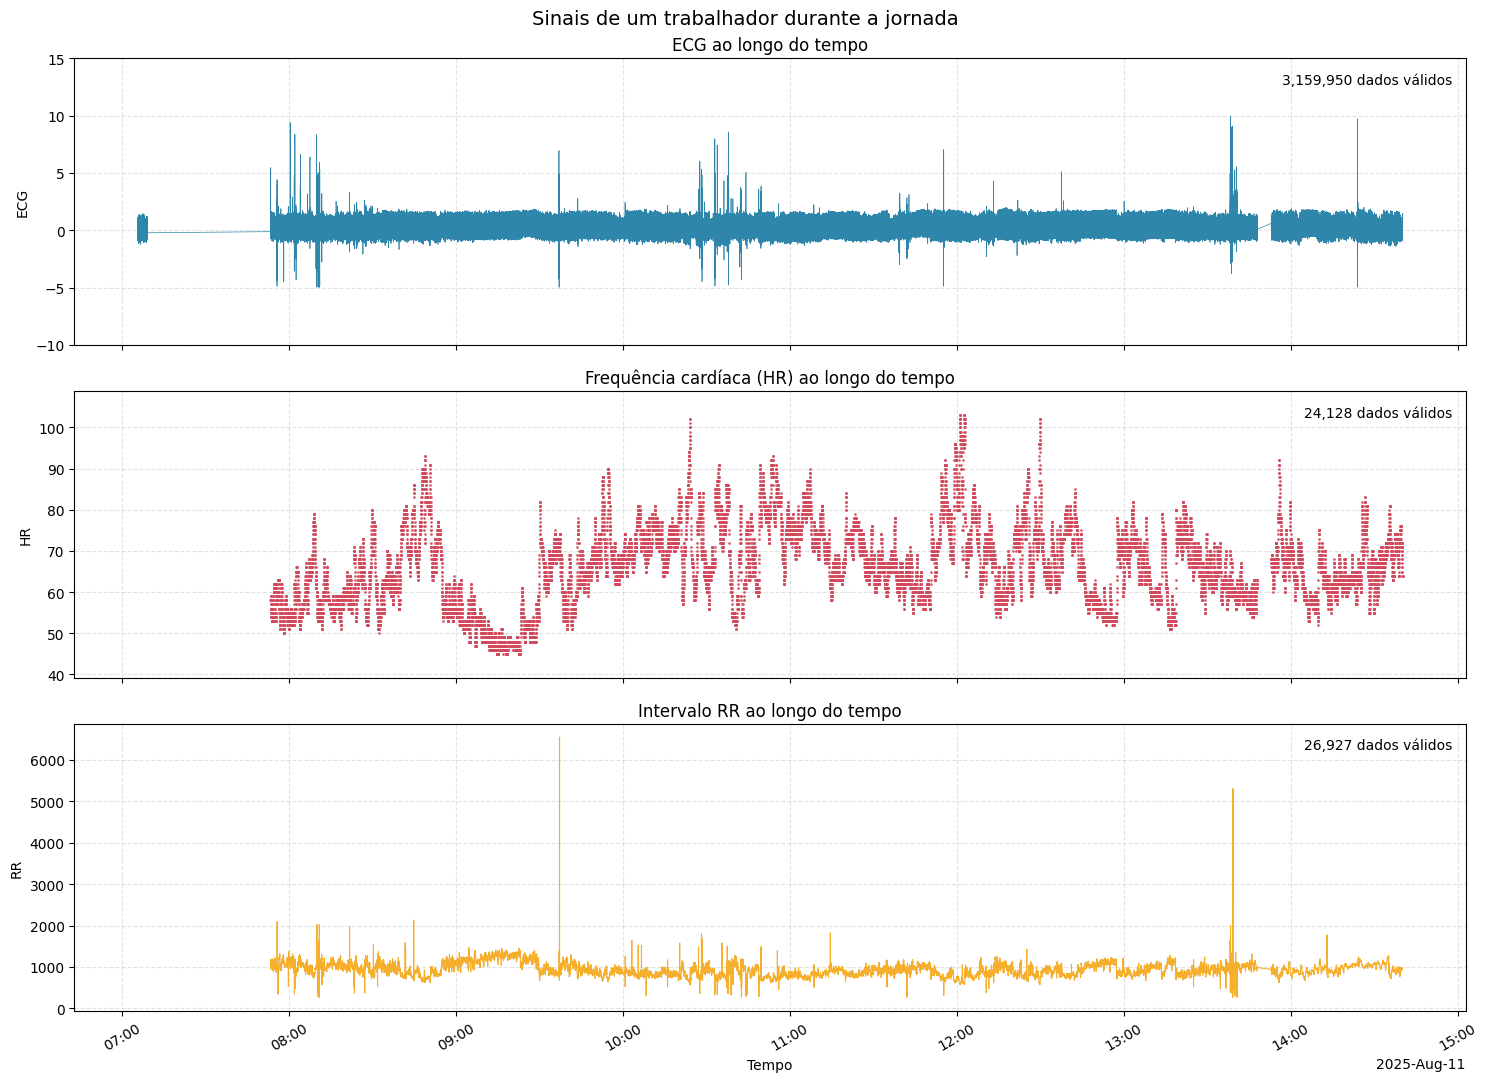
\includegraphics[width=0.85\textwidth]{ch4/assets/señalespolar.png}
\caption{Sinais fisiológicos de um trabalhador durante uma jornada laboral, recolhidos pela banda Polar H10.}
\label{fig:sinais_polar}
\end{figure}

É importante notar que, embora o sensor de ECG opere a uma frequência de 130 Hz, as métricas de HR e RR são registadas apenas com uma cadência aproximada de 1 Hz (um registo por segundo). Esta discrepância de frequências resulta numa elevada densidade de entradas nulas (missing values) nas colunas HR e RR dentro dos ficheiros brutos, uma vez que estas linhas de dados apenas são preenchidas no momento exato em que o algoritmo interno do sensor deteta um novo batimento ou calcula a frequência cardíaca.

\subsubsection*{Relógio Empatica EmbracePlus}

Os dados provenientes do relógio inteligente \textbf{Empatica EmbracePlus} foram obtidos diretamente a partir da plataforma cloud oficial do fabricante em formato CSV. Esta plataforma centraliza a receção dos dados sincronizados pelo dispositivo móvel associado, permitindo a extração dos registos estruturados das variáveis fisiológicas necessárias para a experimentação.

Ao contrário do Polar H10, em que os sinais são armazenados numa única estrutura temporal com elevada frequência de amostragem, o EmbracePlus organiza a informação em \textbf{múltiplos ficheiros CSV independentes}, correspondendo cada ficheiro a uma variável fisiológica ou comportamental distinta. Neste trabalho foi utilizado um único relógio, que foi usado pelo mesmo trabalhador durante vários dias de atividade laboral, permitindo acompanhar continuamente a evolução dos seus indicadores fisiológicos ao longo das diferentes jornadas.

A utilização de um único dispositivo e de um único participante constitui uma \textbf{limitação} deste conjunto de dados. Esta opção resultou das condições específicas do projeto, cujos dados foram recolhidos em simulações de obra e envolveram a participação remunerada de trabalhadores, bem como do \textbf{custo elevado} do relógio Empatica EmbracePlus, que condicionou a disponibilidade de equipamentos. Reconhece-se que a utilização do dispositivo por vários participantes permitiria obter uma maior diversidade interindividual e avaliar de forma mais robusta a capacidade de generalização dos modelos. A recolha de dados de um número maior de participantes constitui uma melhoria importante para trabalho futuro.

Cada dia de recolha origina um conjunto de \textbf{16 ficheiros CSV}, contendo aproximadamente \textbf{1441 registos}, correspondentes a uma resolução temporal de \textbf{1 minuto} ao longo das 24 horas do dia (00:00--23:59). De forma geral, todos os ficheiros apresentam uma estrutura semelhante, composta pelas seguintes colunas:

\begin{itemize}
\item \textbf{timestamp\_unix:} marcação temporal em formato UNIX;
\item \textbf{timestamp\_iso:} representação da data e hora em formato ISO 8601;
\item \textbf{participant\_full\_id:} identificador único do participante;
\item \textbf{Variável fisiológica ou comportamental:} correspondente ao nome do respetivo ficheiro CSV.
\end{itemize}

Na Figura~\ref{fig:sinais_relogio} apresentam-se alguns exemplos de dados fisiológicos e comportamentais recolhidos pelo Empatica EmbracePlus ao longo de um dia.

\begin{figure}[H]
\centering
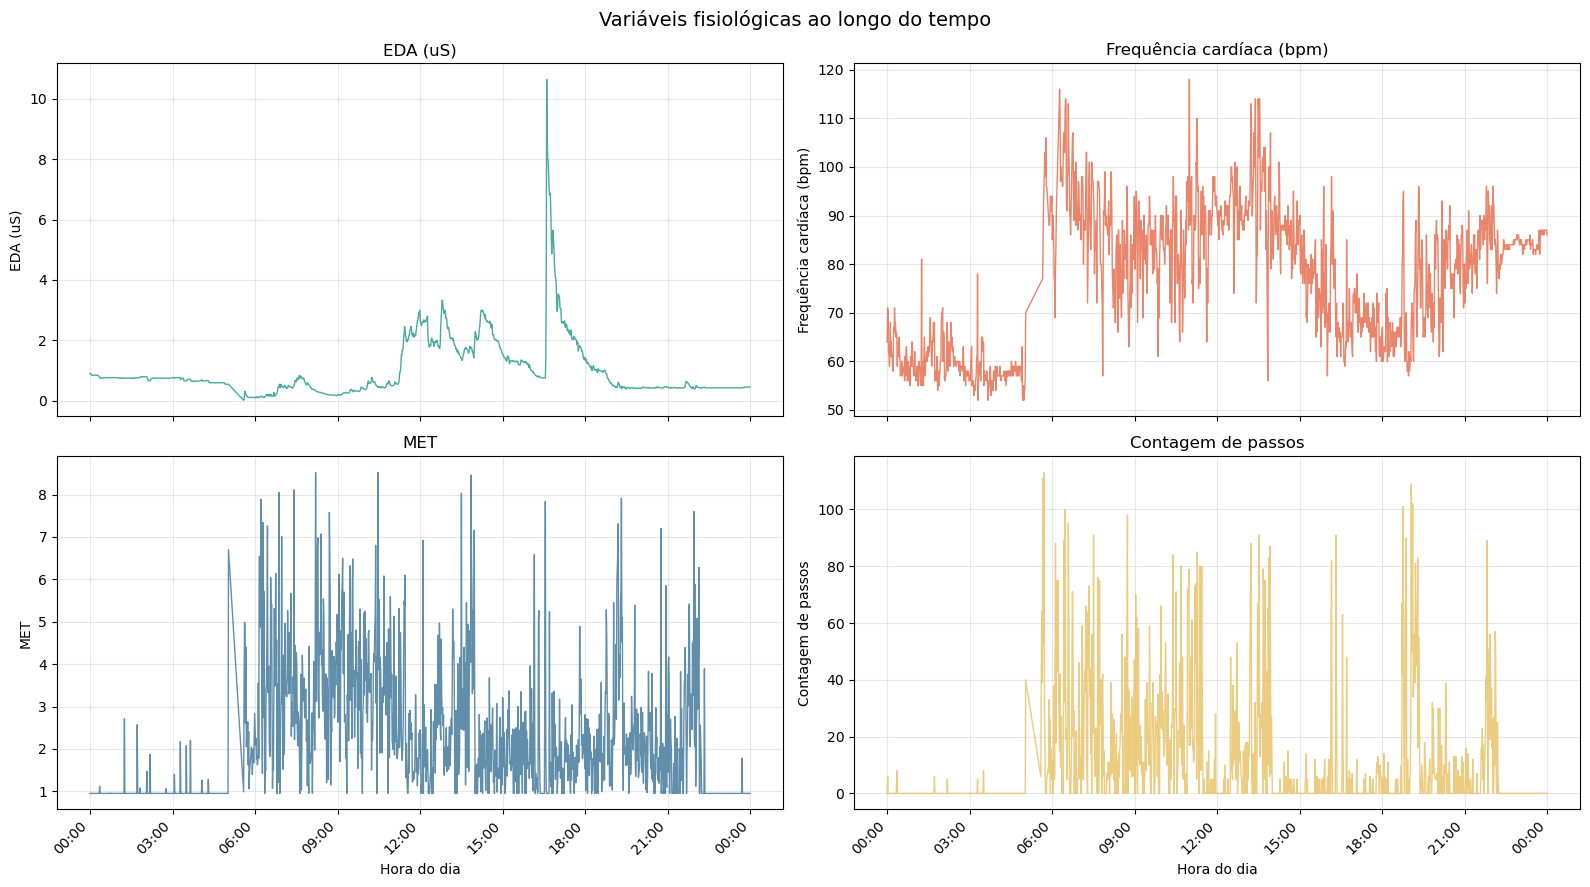
\includegraphics[width=0.90\textwidth]{ch4/assets/señalesreloj.png}
\caption{Evolução temporal de variáveis fisiológicas e comportamentais recolhidas pelo Empatica EmbracePlus.}
\label{fig:sinais_relogio}
\end{figure}

Entre as variáveis disponibilizadas pela plataforma encontram-se diversos indicadores de atividade física, movimento corporal, resposta fisiológica e comportamento, incluindo métricas derivadas do acelerómetro, frequência cardíaca, atividade eletrodérmica (EDA), temperatura cutânea, taxa respiratória, variabilidade da frequência cardíaca (PRV/HRV), intensidade de atividade, gasto energético (MET), número de passos, deteção de sono e utilização do dispositivo.

É importante salientar que algumas variáveis apresentam limitações inerentes ao algoritmo de processamento do próprio dispositivo. Em particular, as métricas de \textbf{Pulse Rate Variability (PRV)} e \textbf{Respiratory Rate} apenas são estimadas quando o utilizador se encontra em repouso ou durante o período de sono. Consequentemente, durante a maior parte da jornada laboral estas variáveis permanecem sem valores válidos, originando uma elevada percentagem de \textit{missing values}. Esta característica foi posteriormente considerada durante a fase de pré-processamento e seleção das variáveis utilizadas no modelo.

%\subsection{Limpeza de Ruído}
%
%Como tratámos os dados atípicos (outliers).

\subsection{Tratamento de Dados em Falta e Limpeza de Ruído}
\label{sec:tratamento-dados-falta}

A presença de dados ruidosos, artefactos de movimento e períodos com ausência de sinal é comum na monitorização fisiológica em ambientes industriais reais. O tratamento e limpeza diferem consoante o tipo de dispositivo e as variáveis medidas de forma a assegurar a qualidade dos dados para os modelos.

\subsubsection*{Banda Peitoral Polar H10}

Como já se mencionou, os sinais de ECG apresentavam registos constantes, enquanto os de frequência cardíaca (HR) e intervalos R-R (RR) registavam apenas um valor por segundo, gerando muitas lacunas aparentes. Esta situação não representava um erro dos dados, mas sim a natureza da aquisição. No entanto, verificaram-se períodos de várias horas em que estas medições estavam ausentes, provavelmente devido a ruído ou falhas temporárias nos sensores, limitando a quantidade de dados disponíveis. Considerando estas circunstâncias, não foi adequada a imputação de valores médios ou de qualquer outra técnica de preenchimento. Em vez disso, à semelhança do procedimento adotado por Smiley et al.~\cite{smiley2023}, nas experiências realizadas optou-se por agrupar os registos em janelas temporais de 30 ou 60 segundos, consoante a experiência, e calcular métricas agregadas, permitindo obter representações robustas de todas as variáveis e minimizar o efeito de lacunas e artefactos pontuais.

Esta agregação temporal revelou-se particularmente adequada para os algoritmos de aprendizagem automática utilizados, dado que a elevada frequência de amostragem do ECG (aproximadamente 130 Hz, um registo a cada 7 ms) combinada com HR e RR mais espaçados (cerca de 1 s) resultava em muitas linhas "vazias" para estas variáveis. As janelas temporais de 30 ou 60 segundos foram definidas com o objetivo de proporcionar uma representação mais consistente dos dados por instância, contribuindo para a estabilidade das características e para a análise da capacidade de generalização dos modelos. Esta diferença na completude dos dados pode ser observada na Tabela~\ref{tab:completude_dados_polar}.

\begin{table}[H]
\centering
\caption{Completude dos dados antes e depois das janelas de 30 segundos.}
\label{tab:completude_dados_polar}
\small
\setlength{\tabcolsep}{2pt}
\begin{tabular}{@{}p{0.24\textwidth} >{\raggedleft\arraybackslash}p{0.12\textwidth} >{\raggedleft\arraybackslash}p{0.20\textwidth} >{\raggedleft\arraybackslash}p{0.12\textwidth} >{\raggedleft\arraybackslash}p{0.25\textwidth}@{}}
\toprule
\textbf{Fonte} & \textbf{Total de linhas} & \textbf{Linhas com algum dado em falta} & \textbf{Linhas completas} & \textbf{Percentagem de linhas com dados em falta} \\
\midrule
Dados brutos & 3160177 & 3139392 & 20785 & 99,34\% \\
Características processadas por janela & 813 & 0 & 813 & 0,00\% \\
\bottomrule
\end{tabular}%
\end{table}

\subsubsection*{Relógio Empatica EmbracePlus}

Os dados provenientes do Empatica EmbracePlus apresentam uma estrutura temporal uniforme, com um registo por minuto para todas as variáveis disponibilizadas pela plataforma. Apesar desta uniformidade, foi realizada uma análise dos valores em falta (\textit{missing values}), verificando-se que a maioria das variáveis fisiológicas e comportamentais apresentava apenas uma reduzida percentagem de registos ausentes (aproximadamente entre 2\% e 4\%). Em contrapartida, as variáveis PRV e Respiratory Rate apresentavam cerca de 75\% e 74\% de valores em falta, respetivamente, característica inerente aos algoritmos proprietários de processamento do Empatica EmbracePlus, pelo que foram posteriormente excluídas durante a etapa de seleção de características. A distribuição detalhada dos valores em falta é apresentada na Tabela~\ref{tab:missing_empatica}.

\begin{table}[H]
\centering
\caption{Percentagem de valores em falta nas variáveis do Empatica EmbracePlus.}
\label{tab:missing_empatica}
\scriptsize
\setlength{\tabcolsep}{3pt}
\begin{tabular}{p{0.24\textwidth} p{0.53\textwidth} c}
\toprule
\textbf{Sinal} & \textbf{Variável analisada} & \textbf{Valores em falta (\%)} \\
\midrule
PRV & \texttt{prv\_rmssd\_ms} & 74,86 \\
Respiratory Rate & \texttt{respiratory\_rate\_brpm} & 73,89 \\
Pulse Rate & \texttt{pulse\_rate\_bpm} & 3,54 \\
Body Position & \texttt{body\_position\_right}, \texttt{body\_position\_left} & 2,64; 2,64 \\
Accelerometers-STD & \texttt{accelerometers\_std\_g} & 2,57 \\
Actigraphy Counts & \texttt{counts\_y\_axis}, \texttt{counts\_x\_axis}, \texttt{counts\_z\_axis}, \texttt{vector\_magnitude} & 2,57 (cada) \\
ActiCounts & \texttt{acticounts\_z\_axis}, \texttt{acticounts\_y\_axis}, \texttt{acticounts\_x\_axis} & 2,57 (cada) \\
Activity Counts & \texttt{activity\_counts} & 2,57 \\
EDA & \texttt{eda\_scl\_usiemens} & 2,57 \\
Activity Intensity & \texttt{activity\_intensity} & 2,57 \\
Activity Classification & \texttt{activity\_class} & 2,57 \\
MET & \texttt{met} & 2,57 \\
Sleep Detection & \texttt{sleep\_detection\_stage} & 2,57 \\
Step Counts & \texttt{step\_counts} & 2,57 \\
Temperature & \texttt{temperature\_celsius} & 2,57 \\
Wearing Detection & \texttt{wearing\_detection\_percentage} & 2,57 \\
\bottomrule
\end{tabular}
\end{table}

As Figuras~\ref{fig:prv_missing} e~\ref{fig:respiratory_rate_missing} ilustram visualmente os períodos sem valores válidos observados nas variáveis PRV e Respiratory Rate, respetivamente. Estes intervalos prolongados ajudam a explicar a elevada percentagem de valores em falta apresentada na Tabela~\ref{tab:missing_empatica}.

\begin{figure}[H]
\centering
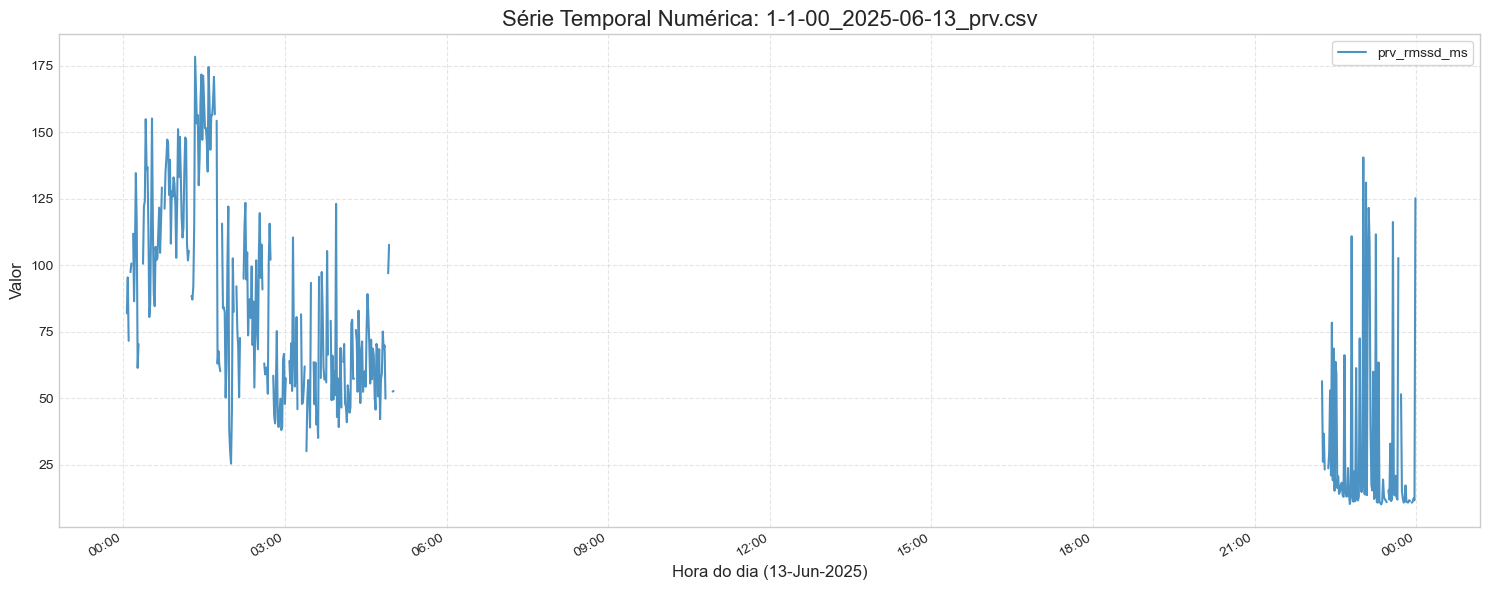
\includegraphics[width=0.95\textwidth]{ch4/assets/PRV.png}
\caption{Série temporal da variável PRV-RMSSD, evidenciando os períodos sem valores registados.}
\label{fig:prv_missing}
\end{figure}

\begin{figure}[H]
\centering
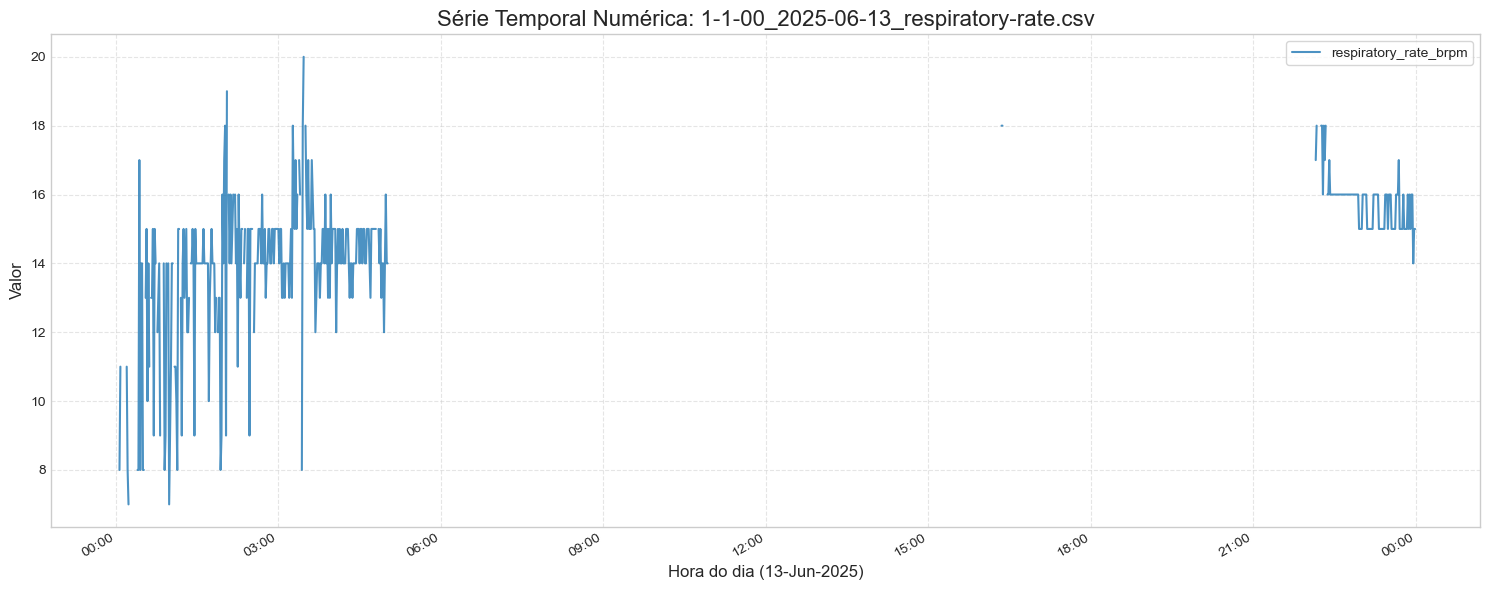
\includegraphics[width=0.95\textwidth]{ch4/assets/respirtionrate.png}
\caption{Série temporal da variável Respiratory Rate, evidenciando os períodos sem valores registados.}
\label{fig:respiratory_rate_missing}
\end{figure}

Considerando que as restantes variáveis apresentavam apenas pequenas lacunas temporais, foi aplicada uma estratégia de imputação diferenciada de acordo com a natureza dos dados. Para as variáveis numéricas contínuas (EDA, Pulse Rate, MET, Activity Counts, Step Counts, Temperature e Vector Magnitude) foi utilizada \textbf{interpolação linear (\textit{Linear Interpolation})}, que estima os valores em falta a partir da tendência definida pelos registos imediatamente anteriores e posteriores, permitindo preservar a continuidade temporal dos sinais fisiológicos.

Por sua vez, para as variáveis categóricas Activity Intensity e Sleep Detection Stage foi aplicado o método \textbf{preenchimento progressivo (\textit{Forward Fill})}, que consiste em propagar o último valor válido observado até ao instante em que um novo valor esteja disponível. Esta abordagem revelou-se adequada, uma vez que estas variáveis representam estados discretos que tendem a manter-se durante períodos consecutivos, tornando inadequada a utilização de métodos de interpolação numérica.

Adicionalmente, procedeu-se à deteção e tratamento de valores anómalos (\textit{outliers}) nas variáveis utilizadas no treino dos modelos. Em vez de recorrer a métodos estatísticos, como o intervalo interquartil (\textit{Interquartile Range} – IQR) ou o \textit{Z-score}, optou-se por uma abordagem heurística baseada em limites fisiologicamente plausíveis para cada biomarcador. Para o tratamento destes valores foi utilizada a técnica de clipping, que consiste em limitar os valores de uma variável a um intervalo previamente definido, substituindo apenas os valores inferiores ao limite mínimo pelo respetivo limite inferior e os valores superiores ao limite máximo pelo limite superior, preservando assim todas as observações do conjunto de dados. Os limites adotados para cada variável são apresentados na Tabela \ref{tab:limites_fisiologicos}.

Os limites adotados foram estabelecidos com base em referências clínicas e biomecânicas. Por exemplo, o estudo PainFREE Rx II \cite{wathen2004} analisou episódios de taquicardia ventricular rápida entre 188 e 250 bpm, sustentando a definição de 250 bpm como limite superior para a variável Pulse Rate; o estudo de Štuhec et al. \cite{stuhec2023}, centrado no desempenho de Usain Bolt no sprint, serviu de referência para definir o limite de 300 passos/min para a variável Step Counts. Para as restantes medidas, nomeadamente EDA, MET, Activity Counts e Vector Magnitude, aplicou-se o mesmo princípio, definindo limites compatíveis com a natureza e a escala de cada variável para controlar valores implausíveis ou resultantes de artefactos.

Após o tratamento dos dados em falta, obteve-se um conjunto de dados consistente e sem valores ausentes nas variáveis consideradas para o treino dos modelos, garantindo a qualidade necessária para as etapas seguintes de engenharia de características e aprendizagem automática.

\begin{table}[H]
\centering
\caption{Limites fisiológicos utilizados para a deteção e tratamento de valores anómalos}
\label{tab:limites_fisiologicos}
\begin{tabular}{@{}lccc@{}}
\toprule
Variável & Limite mínimo & Limite máximo & Unidade \\
\midrule
Pulse Rate & 0 & 250 & bpm \\
EDA & 0 & 50 & µS \\
MET & 0,5 & 20 & MET \\
Step Counts & 0 & 300 & passos/min \\
Activity Counts & 0 & 100000 & contagens \\
Vector Magnitude & 0 & 50000 & unidades \\
\bottomrule
\end{tabular}
\end{table}

\subsection{Engenharia e Seleção de Características}

Após a conclusão das etapas anteriores, procedeu-se à engenharia e seleção de características. Este processo envolveu tanto a criação de novas métricas quantitativas a partir dos sinais fisiológicos brutos quanto a filtragem das variáveis mais relevantes para descrever o estado dos trabalhadores. Esta fase é determinante para converter dinâmicas corporais complexas em entradas estruturadas, otimizando o desempenho e a capacidade de generalização dos modelos de aprendizagem automática.

\subsubsection*{Características da Banda Peitoral Polar H10}

As características utilizadas nos modelos foram obtidas através de um processo de engenharia de características aplicado aos sinais do Polar H10. Para além das variáveis de identificação, de tempo e de atividade, foram calculadas características de qualidade do sinal, métricas derivadas do ECG, indicadores de variabilidade da frequência cardíaca e variáveis temporais. As variáveis de identificação e de tempo, como \texttt{Trabajador}, \texttt{UNIX Timestamp}, \texttt{DateTime} e \texttt{Actividad}, foram mantidas para organizar os registos, sincronizar as observações e contextualizar cada janela, não constituindo, por si só, características fisiológicas de entrada dos modelos.

\paragraph{Variáveis de Qualidade e ECG:}

Do sinal de ECG agregaram-se métricas estatísticas em cada janela temporal de 30 ou 60 segundos, dependendo da experiência, incluindo:

\begin{itemize}
\item \textbf{Média (ECG\_mean):} valor médio do sinal, que representa o nível geral da atividade elétrica cardíaca.
\item \textbf{Desvio padrão (ECG\_std):} variabilidade do sinal dentro da janela, permitindo capturar instabilidade cardíaca.
\item \textbf{Amplitude ou alcance (ECG\_range):} diferença entre valor máximo e mínimo, indicando variações abruptas.
\item \textbf{Energia do sinal (ECG\_energy):} soma dos quadrados dos valores do sinal, correlacionando-se com intensidade do batimento~\cite{pantompkins1985}.
\item \textbf{Entropia amostral (ECG\_samp\_ent):} mede a complexidade do sinal e irregularidades que podem indicar stress ou fadiga~\cite{richman2000}.
\item \textbf{Número de picos perdidos (ECG\_missing\_peaks):} indica falhas na detecção de batimentos, útil para identificar artefactos ou irregularidades fisiológicas~\cite{adarri2017}.
\item \textbf{HR\_valid:} indicador da validade ou disponibilidade do valor de frequência cardíaca na respetiva janela.
\end{itemize}

\paragraph{Variáveis de HRV e Frequência Cardíaca:}
A partir dos intervalos R-R calcularam-se métricas clássicas de HRV em cada janela, nomeadamente SDNN, RMSSD e pNN50, cujas definições podem ser consultadas em~\cite{shaffer2017}:
\begin{itemize}
\item \textbf{SDNN:} desvio padrão dos intervalos RR, indicador de variabilidade geral.
\item \textbf{RMSSD:} raiz quadrada da média dos quadrados das diferenças sucessivas, sensível ao sistema nervoso parassimpático.
\item \textbf{pNN50:} percentagem de diferenças consecutivas superiores a 50 ms, outro marcador de HRV.
\item \textbf{HR\_mean, HR\_max, HR\_min:} valores médio, máximo e mínimo da frequência cardíaca, fornecendo informação sobre esforço e recuperação.
\end{itemize}

\paragraph{Variáveis Temporais:}
Para representar a evolução dos sinais ao longo do tempo, foram ainda calculadas as seguintes variáveis, inspiradas no estudo~\cite{predictingdailyrecovery2024}:
\begin{itemize}
\item \textbf{HR\_mean\_ultimos\_5min:} média da frequência cardíaca nas cinco janelas anteriores, permitindo incorporar informação recente.
\item \textbf{cambio\_HR\_vs\_baseline:} diferença entre a frequência cardíaca observada e o valor de referência do trabalhador.
\item \textbf{tendencia\_HR:} direção da evolução da frequência cardíaca ao longo das janelas temporais.
\item \textbf{cambio\_RMSSD:} variação da RMSSD relativamente ao valor de referência.
\end{itemize}

A escolha e criação destas características baseia-se em estudos sobre stress e fadiga fisiológica~\cite{karthikeyan2023,mental_fatigue_ablation2025,ardecani2025}. As métricas calculadas a partir do ECG refletem a intensidade e complexidade da atividade elétrica do coração, enquanto as métricas de HRV e frequência cardíaca fornecem informação sobre a resposta autonómica e o equilíbrio entre esforço e recuperação. As variáveis temporais acrescentam contexto sobre a evolução recente dos sinais e sobre os desvios relativamente ao baseline individual. A agregação em janelas de 30 ou 60 segundos garante que cada instância de treino contenha dados suficientes para representar de forma robusta o estado do trabalhador, minimizando o efeito de lacunas ou artefactos pontuais.

\paragraph{Variáveis Estandardizadas:}
Para além das versões originais, cada variável fisiológica e temporal utilizada pelos modelos possui uma versão estandardizada com o sufixo \texttt{\_z}. Estas versões foram calculadas relativamente ao baseline do registo, através da Equação~\ref{eq:zscore-caracteristicas}:

\begin{equation}
z = \frac{x - \mu_{baseline}}{\sigma_{baseline}}
\label{eq:zscore-caracteristicas}
\end{equation}

em que $x$ representa o valor da variável na janela, $\mu_{baseline}$ corresponde à média da variável no baseline e $\sigma_{baseline}$ ao respetivo desvio padrão no baseline. Esta transformação coloca as variáveis numa escala comparável e permite avaliar cada observação relativamente ao padrão fisiológico de referência do trabalhador. Assim, por exemplo, \texttt{HR\_mean} possui a correspondente versão \texttt{HR\_mean\_z}; o mesmo princípio aplica-se às restantes variáveis fisiológicas e temporais utilizadas.

Estas features servem de base para o FatigueIndex, que combina várias métricas normalizadas para gerar um valor contínuo representativo do estado de fadiga. Este índice é utilizado posteriormente como target em tarefas de regressão ou categorização.

\subsubsection*{Características do Relógio Empatica EmbracePlus}

Ao contrário da banda peitoral Polar H10, na qual foi necessário criar novas características a partir dos poucos sinais extraídos de ECG e HR, o Relógio Empatica EmbracePlus disponibiliza um conjunto de variáveis fisiológicas e comportamentais previamente processadas pelos algoritmos proprietários da plataforma. Consequentemente, a etapa de engenharia de características centrou-se sobretudo na seleção das variáveis mais relevantes, na codificação das variáveis categóricas e na agregação temporal dos dados, de forma a obter um conjunto de características adequado para os modelos de aprendizagem automática.

Inicialmente, a plataforma disponibilizava um conjunto alargado de variáveis, tal como destacado nas secções anteriores. Contudo, verificou-se que várias destas métricas poderiam ser redundantes, apresentar pouca relevância para a deteção dos estados psicofisiológicos pretendidos ou, inclusive, conter uma elevada percentagem de valores em falta que inviabilizaria a continuidade da análise.

Em particular, as variáveis PRV-RMSSD (\textit{Pulse Rate Variability}) e Respiratory Rate apresentavam aproximadamente 75\% de valores em falta. Esta elevada proporção de dados ausentes está relacionada com as condições específicas em que o algoritmo do EmbracePlus disponibiliza estas métricas, nomeadamente períodos de repouso e sono, resultando numa cobertura temporal substancialmente inferior à das restantes variáveis analisadas. Consequentemente, a sua inclusão conduziria a uma redução significativa do número de observações efetivamente disponíveis para análise e a uma menor comparabilidade com as restantes medidas fisiológicas, sobretudo durante os períodos de atividade laboral.

Além disso, a ausência destes valores está condicionada ao estado comportamental e fisiológico do participante. Assim, a aplicação de métodos convencionais de imputação poderia introduzir pressupostos pouco adequados sobre a evolução destas variáveis e potencialmente enviesar os resultados. Face a estas limitações de disponibilidade e cobertura temporal, optou-se por excluir a PRV-RMSSD e a Respiratory Rate das análises finais, privilegiando variáveis com maior completude e maior consistência na cobertura dos períodos de interesse do estudo.

Após esta análise, foi definido um conjunto reduzido de variáveis consideradas mais representativas para a deteção de estados fisiológicos associados à fadiga, incluindo:

\begin{itemize}
\item \textbf{EDA (eda\_scl\_usiemens):} indicador da atividade eletrodérmica, diretamente associado à ativação do sistema nervoso simpático e frequentemente utilizado como biomarcador de stress.
\item \textbf{Pulse Rate (pulse\_rate\_bpm):} frequência cardíaca média, representando a resposta cardiovascular do trabalhador.
\item \textbf{MET:} estimativa do gasto energético metabólico durante a atividade.
\item \textbf{Activity Counts:} indicador global do nível de atividade física.
\item \textbf{Step Counts:} número de passos realizados em cada minuto.
\item \textbf{Vector Magnitude:} magnitude do movimento corporal obtida a partir do acelerómetro.
\item \textbf{Activity Class:} classificação automática do tipo de atividade realizada.
\item \textbf{Activity Intensity:} nível de intensidade da atividade física.
\item \textbf{Sleep Detection Stage:} indicador do estado de vigília ou sono.
\end{itemize}

As variáveis categóricas foram posteriormente transformadas em formato numérico para permitir a sua utilização pelos algoritmos de aprendizagem automática. A variável \textbf{Activity Class} foi codificada através de \textbf{One-Hot Encoding}, originando uma coluna binária para cada categoria (\textit{STILL}, \textit{WALKING} e \textit{GENERIC}). Esta abordagem foi escolhida porque estas categorias representam estados independentes, sem qualquer relação de ordem entre si, evitando que o modelo interprete artificialmente uma categoria como superior ou inferior a outra.

Por outro lado, as variáveis \textbf{Activity Intensity} e \textbf{Sleep Detection Stage} foram convertidas recorrendo a \textbf{Ordinal Encoding}. No caso da intensidade da atividade, existe uma progressão natural entre os diferentes níveis (\textit{Sedentary}, \textit{LPA}, \textit{MPA} e \textit{VPA}), permitindo representá-los pelos valores 0, 1, 2 e 3. De forma semelhante, a variável \textbf{Sleep Detection Stage} foi simplificada para distinguir apenas entre estado de vigília e estado de sono, agrupando as diferentes fases de sono numa única categoria, uma vez que o objetivo do estudo não era analisar a arquitetura do sono, mas apenas identificar períodos de descanso e recuperação fisiológica.

Finalmente, a fase experimental considerou dois níveis de granularidade temporal. Numa primeira abordagem, utilizaram-se os registos originais do EmbracePlus (amostragem de um minuto), totalizando cerca de 1440 observações por dia. Na segunda, aplicou-se uma agregação em janelas de 10 minutos através do cálculo da média, reduzindo o volume para 144 registos diários. Esta estratégia visou estabilizar os sinais fisiológicos, permitindo identificar tendências de maior duração e avaliar o impacto da resolução temporal no desempenho dos modelos.

\section{Modelação do Problema e Definição dos Modelos}

Nesta secção, explicam-se os modelos de Inteligência Artificial escolhidos para prever os estados de fadiga e stress dos trabalhadores. O foco foi selecionar algoritmos capazes de analisar as variações dos sinais ao longo do tempo para identificar padrões de comportamento. Além da descrição de cada modelo, apresentam-se as estratégias de treino e os resultados obtidos, demonstrando como o sistema consegue transformar dados técnicos em alertas úteis para a segurança no trabalho através do Gémeo Digital.

\subsection{Escolha do Algoritmo}

A seleção dos algoritmos baseou-se no estado da arte apresentado no Capítulo~\ref{chap:TecnologiasEmergentes}. Como mostram os artigos analisados, os problemas supervisionados com dados fisiológicos e uma variável-alvo recorrem a XGBoost, Random Forest, SVM e modelos lineares~\cite{thomas2025,goutham2025,albarran2025}. Na ausência de etiquetas, estudos específicos recorrem a métodos não supervisionados, como GMM, K-Means e \textit{clustering} hierárquico~\cite{georgiev2026,georgieva2025}. Assim, a escolha considerou a natureza dos dados e a existência de um alvo em cada dispositivo.

Consequentemente, a metodologia foi definida em função da natureza e da disponibilidade dos dados, procurando simultaneamente explorar abordagens de ambas as famílias de aprendizagem. Em ambos os dispositivos não existia uma variável-alvo previamente definida para identificar diretamente os estados de fadiga. No caso do Polar H10, o conjunto de dados era mais limitado e centrado principalmente em variáveis numéricas cardiovasculares, pelo que foi construído o \textit{FatigueIndex} a partir das características fisiológicas extraídas, cujo cálculo é explicado na secção seguinte, permitindo utilizá-lo como variável-alvo e formular o problema como uma tarefa de \textbf{aprendizagem supervisionada}, através de modelos de regressão e classificação.

Por outro lado, o Empatica EmbracePlus disponibilizava um conjunto de dados mais diversificado, incluindo variáveis de diferentes dimensões fisiológicas e comportamentais. Neste caso, optou-se por não definir previamente uma variável-alvo, explorando a estrutura dos dados através de uma abordagem de \textbf{aprendizagem não supervisionada}, baseada em \textit{clustering}, permitindo identificar possíveis padrões ou perfis nos dados sem impor previamente classes de fadiga. Assim, as duas abordagens permitiram analisar o problema de forma complementar.

\subsubsection*{Algoritmos para a Banda Peitoral Polar H10}

Para a banda Polar H10, focada na análise da fadiga e do esforço físico através de regressão e classificação, foram selecionados cinco algoritmos principais:

\begin{itemize}
\item \textbf{Regressão Linear:} escolhida pela sua simplicidade e interpretabilidade. Permite avaliar relações lineares diretas entre as features e o target, funcionando como baseline para comparação com modelos mais complexos.
\item \textbf{XGBoost (Regressor e Classifier):} modelos baseados em árvores que capturam relações não lineares e interações complexas entre as variáveis. O Regressor permite prever valores contínuos, enquanto o Classifier trabalha com labels categóricos. XGBoost foi escolhido pela sua robustez, capacidade de generalização e bom desempenho em dados com variabilidade e ruído.
\item \textbf{Support Vector Machine (SVM) com kernel RBF:} modelo não linear que projeta os dados num espaço de alta dimensão para encontrar fronteiras de decisão complexas. O kernel RBF permite capturar padrões subtis que não seriam detectáveis por modelos lineares, sendo útil tanto para regressão (SVR) como para classificação (SVC).
\item \textbf{Logistic Regression:} modelo linear utilizado para classificação, que estima a probabilidade de pertença de cada observação às diferentes classes de fadiga. A sua simplicidade e interpretabilidade permitem comparar o desempenho de uma abordagem linear com os modelos não lineares.
\item \textbf{Random Forest:} ensemble de árvores de decisão que combina as previsões de várias árvores treinadas com diferentes amostras e subconjuntos de características. Este algoritmo permite modelar relações não lineares e reduzir a dependência de uma única árvore, sendo adequado para dados com interações entre variáveis fisiológicas.
\end{itemize}

Em conjunto, estes modelos abrangem diversos níveis de complexidade, desde abordagens lineares a modelos baseados em árvores e máquinas de vetores de suporte. Esta diversidade permite comparar o desempenho de cada técnica na análise da fadiga e do esforço físico, avaliando o impacto da complexidade na precisão e capacidade de generalização das previsões.

\subsubsection*{Algoritmos para o Relógio Empatica EmbracePlus}

Devido à natureza multidimensional dos dados do Empatica EmbracePlus, que integra múltiplos indicadores fisiológicos e comportamentais, e à inexistência de um label que representasse diretamente os estados de fadiga, a exploração centrou-se em algoritmos de clustering. O objetivo foi identificar padrões naturais nos dados, permitindo identificar diferentes estados fisiológicos e comportamentais sem a necessidade de categorias previamente definidas.

\begin{itemize}
\item \textbf{Gaussian Mixture Model (GMM):} modelo probabilístico adequado para dados fisiológicos, permitindo representar transições graduais entre diferentes estados através de probabilidades de pertença aos clusters. O número de clusters foi determinado com base no \textit{Bayesian Information Criterion} (BIC), selecionando a configuração que apresentou o melhor equilíbrio entre qualidade do ajuste e complexidade do modelo.
\item \textbf{Clustering Hierárquico Aglomerativo:} método que organiza progressivamente as observações numa estrutura hierárquica (dendrograma), facilitando a interpretação das relações entre os diferentes grupos. Neste trabalho foi utilizada a estratégia de ligação Ward com distância euclidiana. A seleção do número de clusters foi suportada pela análise do dendrograma, complementada pelo \textit{Silhouette Score} e pela curva do cotovelo (\textit{Elbow Method}).
\end{itemize}

O algoritmo K-Means foi utilizado apenas na fase exploratória para apoiar a análise da curva do cotovelo e determinar o número de clusters. Adicionalmente, compararam-se os resultados da seleção automática com configurações de clusters previamente definidas, permitindo validar a estrutura dos agrupamentos.

A combinação destas abordagens permite explorar os dados fisiológicos sob perspetivas probabilísticas e estruturais complementares. Esta sinergia facilita a identificação de padrões complexos captados pelo relógio inteligente e a sua associação a diferentes níveis de ativação do utilizador.

\subsection{Definição de alvos para aprendizagem supervisionada}

Como os dados brutos e as características extraídas dos dispositivos portáteis não contêm classificações prévias diretas (etiquetas ou labels) para estados psicofisiológicos complexos como a fadiga ou o nível de stress, tornou-se imperativo definir targets analíticos para supervisionar o treino dos modelos.

\subsubsection*{Cálculo da Variável Alvo para o Polar H10}
\label{sec:fatigueindex}

Os dados adquiridos através da banda Polar H10 não continham um label direto que identificasse estados complexos como fadiga, cansaço ou stress. As variáveis disponíveis, como ECG, HR e HRV, fornecem apenas sinais fisiológicos brutos, que por si só não indicam de forma explícita o estado subjetivo do trabalhador. Por conseguinte, tornou-se necessário criar uma representação quantitativa que pudesse servir como target para os modelos de aprendizagem automática.

\paragraph{FatigueIndex: contínuo}

Uma abordagem possível foi a construção manual de um \textit{label} contínuo, designado como \textit{FatigueIndex}, através de uma combinação heurística de características fisiológicas extraídas dos sinais de frequência cardíaca (HR), variabilidade da frequência cardíaca (HRV) e eletrocardiograma (ECG), seguindo uma abordagem semelhante à utilizada por Karthikeyan et al.~\cite{karthikeyan2023}, que propuseram uma anotação heurística de fadiga baseada em características fisiológicas derivadas do ECG e da HRV. No presente trabalho, esta abordagem foi adaptada às características disponíveis e aos objetivos da investigação.

Para a construção do \textit{FatigueIndex}, as \textit{features} foram previamente estandardizadas utilizando o \textit{z-score}, de forma a colocar as diferentes características numa escala comum, com média igual a 0 e desvio padrão igual a 1. A estandardização é calculada segundo a Equação~\ref{eq:zscore-fatigueindex}:

\begin{equation}
z = \frac{x - \mu}{\sigma}
\label{eq:zscore-fatigueindex}
\end{equation}

onde:

$x$ é o valor original da feature, $\mu$ é a média da feature, $\sigma$ é o desvio padrão da feature.

O FatigueIndex é calculado como uma combinação linear ponderada dos z-scores das features normalizadas, conforme mostrado no seguinte código Python:

\begin{lstlisting}[language=Python, caption=Cálculo do FatigueIndex, label=lst:fatigueindex]
fatigue_index = (
        1.2 * z_scores['HR_mean'] -
        1.0 * z_scores['RMSSD'] -
        0.8 * z_scores['SDNN'] -
        0.8 * z_scores['pNN50'] +
        0.6 * z_scores['ECG_energy'] +
        0.4 * z_scores['ECG_samp_ent'] +
        0.5 * z_scores['ECG_missing_peaks']
    )
\end{lstlisting}

Os coeficientes refletem a importância fisiológica estimada de cada métrica:

\begin{itemize}
\item \textbf{HR\_mean} contribui positivamente, já que frequências cardíacas elevadas indicam maior esforço ou tensão~\cite{marcora2009}.
\item \textbf{RMSSD}, \textbf{SDNN} e \textbf{pNN50} contribuem negativamente, dado que uma maior variabilidade cardíaca está associada a uma maior capacidade de recuperação e a menor fadiga~\cite{pichot2002}.
\item \textbf{ECG\_energy}, \textbf{ECG\_samp\_ent} e \textbf{ECG\_missing\_peaks} adicionam informação sobre intensidade, complexidade e eventuais irregularidades no ECG.
\end{itemize}

O resultado é um valor contínuo que representa de forma relativa o nível de fadiga de cada janela temporal de 30 ou 60 segundos, dependendo da experiência.

\paragraph{FatigueIndex: categórico}

Para os modelos de classificação que requerem \textit{labels} categóricos, o \textit{FatigueIndex} contínuo foi convertido em três classes através da utilização dos percentis 33 e 66 como pontos de corte. Esta abordagem foi inspirada em trabalhos anteriores que utilizaram estes percentis para transformar variáveis contínuas relacionadas com \textit{wellness} e fadiga em três categorias destinadas a problemas de classificação~\cite{rossi2022wellness}. A utilização destes dois pontos de corte corresponde à divisão da distribuição em três grupos de dimensão aproximadamente semelhante, permitindo definir categorias relativas de baixa, média e elevada fadiga sem recorrer a limiares absolutos previamente definidos.

\begin{itemize}
\item Valores abaixo do percentil P33 foram classificados como fadiga baixa;
\item Valores entre os percentis P33 e P66 foram classificados como fadiga média;
\item Valores acima do percentil P66 foram classificados como fadiga elevada.
\end{itemize}

Desta forma, foi possível criar um conjunto de dados com targets tanto contínuos como categóricos, permitindo utilizar diferentes tipos de modelos de aprendizagem automática com o objetivo de prever diferentes estados de atividade ou fadiga, conforme a tarefa de regressão ou classificação.

\subsubsection*{Cálculo da Variável Alvo para o Relógio Empatica EmbracePlus}

Dada a ausência de etiquetas pré-definidas, a abordagem para o relógio Empatica EmbracePlus delegou a identificação de estados aos algoritmos de \textit{clustering}. Esta estratégia de aprendizagem não supervisionada permite que o sistema agrupe os registos com base na sua semelhança estatística, identificando padrões naturais nos dados sem a imposição de fórmulas heurísticas ou um viés analítico prévio.

\subsection{Normalização / Scaling de Features}

A normalização (\textit{feature scaling}) consiste na transformação das variáveis para uma escala comum, de forma a eliminar o efeito das diferenças de magnitude entre as \textit{features}. Neste trabalho foi utilizada a técnica \texttt{StandardScaler}~\cite{scikitlearn2021standardscaler}, que realiza uma estandardização do tipo \textit{z-score}, transformando cada variável de modo a apresentar média igual a 0 e desvio padrão igual a 1.

Esta etapa revelou-se particularmente importante para os algoritmos baseados em distâncias ou na geometria do espaço de características, como o \textit{Support Vector Machine} (SVM), utilizado no processamento dos dados da banda Polar H10, bem como para os algoritmos de \textit{clustering} aplicados aos dados do relógio inteligente Empatica EmbracePlus. Em algoritmos sensíveis à escala, a ausência de normalização pode fazer com que variáveis com amplitudes superiores dominem o cálculo das distâncias, influenciando indevidamente a formação dos \textit{clusters} ou a definição das fronteiras de decisão; a importância desta etapa no treino dos modelos é também discutida e confirmada por Shao et al.~\cite{shao2020normalization}.

Por outro lado, é amplamente reconhecido que os modelos baseados em árvores de decisão, como o XGBoost, são pouco sensíveis à escala das variáveis, uma vez que efetuam divisões com base em limiares e não em métricas de distância~\cite{scikitlearn2026featurescaling}. Ainda assim, a estandardização foi mantida sempre que necessária para garantir consistência entre as diferentes etapas do processamento e dos modelos experimentais.

\subsection{Divisão do Dataset}

\subsubsection*{Banda Peitoral Polar H10}

Para avaliar corretamente o desempenho dos modelos de aprendizagem automática treinados com os dados de um único trabalhador, o conjunto de dados desse trabalhador foi dividido em três partes distintas: \textbf{treino}, \textbf{validação} e \textbf{teste}. Do total de dados disponíveis, 60\% foram utilizados para o treino dos modelos, 20\% para validação e 20\% para teste, seguindo uma estratégia de divisão em três subconjuntos semelhante à utilizada por Tsao et al.~\cite{tsao2018}, que treinaram modelos de aprendizagem automática com dados fisiológicos utilizando esta divisão. O conjunto de treino foi usado para aprender os padrões presentes nos dados, o conjunto de validação para ajustar e comparar diferentes modelos, e o conjunto de teste para avaliar o desempenho final em dados nunca vistos. Esta divisão permite avaliar a capacidade de generalização dos modelos, reduzindo o risco de sobreajuste (overfitting) e garantindo uma estimativa mais fiável do desempenho em novos dados. Como já mencionado anteriormente na Subsecção~\ref{sec:tratamento-dados-falta}, os dados foram agregados em janelas temporais de 30 segundos. As divisões utilizadas podem ser consultadas na Figura~\ref{fig:divisao_treino_validacao_teste}.

\begin{figure}[H]
\centering
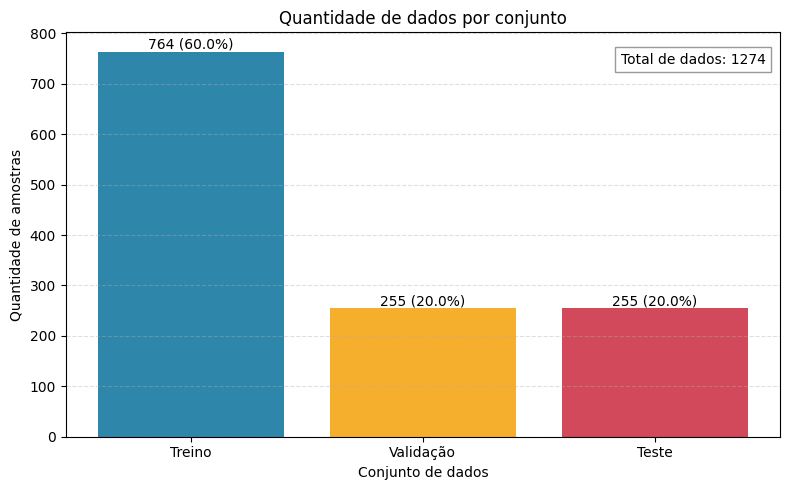
\includegraphics[width=0.8\textwidth]{ch4/assets/TESTVALTRAIN.png}
\caption{Divisão do conjunto de dados em treino, validação e teste.}
\label{fig:divisao_treino_validacao_teste}
\end{figure}

Para os modelos treinados com dados de vários trabalhadores, foi utilizada uma validação cruzada \textit{Leave-One-Subject-Out} (LOSO). Em cada iteração, os dados de um trabalhador foram reservados para teste, enquanto os dados dos restantes trabalhadores foram utilizados para o treino. A seleção dos hiperparâmetros foi realizada através de uma validação cruzada interna estratificada de cinco partições, aplicada exclusivamente aos dados de treino. Esta abordagem foi inspirada em trabalhos como o de Behradfar e Nuamah~\cite{behradfar2025}, que utilizaram uma estratégia de validação cruzada LOSO aninhada para avaliar a generalização de modelos de aprendizagem automática aplicados a características derivadas de sinais ECG. Este procedimento permitiu avaliar a capacidade de generalização dos modelos para trabalhadores não observados durante o treino, reduzindo o risco de sobreajuste e evitando a utilização de informação do trabalhador de teste durante o processo de aprendizagem.

\subsubsection*{Relógio Empatica EmbracePlus}

Ao contrário da abordagem supervisionada adotada para a banda Polar H10, os algoritmos de clustering aplicados aos dados do Empatica EmbracePlus não requerem uma divisão do conjunto de dados em treino, validação e teste, uma vez que o seu objetivo consiste em identificar padrões e agrupamentos naturais existentes nos dados, sem um alvo conhecido a prever. Deste modo, os algoritmos foram aplicados sobre o conjunto completo de dados previamente pré-processado, permitindo explorar toda a informação disponível durante o processo de agrupamento. A seleção do número de clusters foi efetuada com base em critérios internos de avaliação adequados a cada algoritmo.

Esta abordagem permitiu avaliar a qualidade e a consistência dos agrupamentos com base na estrutura interna dos dados, em vez da capacidade preditiva sobre um conjunto de teste independente.

\section{Definição do Ambiente de Experimentação}

Para garantir a reprodutibilidade dos testes e validar o desempenho dos modelos propostos, apresentam-se as especificações detalhadas do ambiente experimental. A configuração de hardware utilizada para o processamento dos dados e treino dos algoritmos é descrita na Tabela \ref{tab:hardware}, enquanto a Tabela \ref{tab:software} detalha o ecossistema de software, incluindo as versões da linguagem de programação e das bibliotecas fundamentais.

A gestão das dependências foi realizada através de um ambiente virtual isolado (venv), assegurando que todos os pacotes e frameworks mantivessem a consistência necessária entre execuções, evitando conflitos de versões e garantindo que os resultados possam ser replicados em sistemas com configurações equivalentes.

\begin{table}[H]
\centering
\caption{Especificações de Hardware da Workstation}
\label{tab:hardware}
\begin{tabular}{@{}ll@{}}
\toprule
Componente & Especificação \\
\midrule
CPU (Processador) & Intel(R) Core(TM) Ultra 7 165H \\
Memória RAM & 32 GB \\
FPU & Integrada na arquitetura CPU Intel Ultra 7 \\
Armazenamento & 1 TB NVMe SSD (Partição GPT) \\
Sistema Operativo & Windows 10 Pro \\
\bottomrule
\end{tabular}
\end{table}

\begin{table}[H]
\centering
\caption{Especificações de Software e Bibliotecas}
\label{tab:software}
\begin{tabular}{@{}ll@{}}
\toprule
Componente / Biblioteca & Versão \\
\midrule
Python & 3.10.11 \\
Pandas & 2.3.3 \\
NumPy & 2.2.6 \\
Scikit-learn & 1.7.2 \\
XGBoost & 3.1.3 \\
SciPy & 1.15.3 \\
Antropy & 0.1.9 \\
Matplotlib & 3.10.8 \\
\bottomrule
\end{tabular}
\end{table}

\section{Avaliação Experimental}

Nesta secção descreve-se a metodologia utilizada para treinar, avaliar e comparar os modelos de Inteligência Artificial desenvolvidos para os dois dispositivos em estudo. Para a banda peitoral Polar H10, são apresentados os resultados obtidos nas tarefas de regressão, utilizando o FatigueIndex contínuo como variável-alvo, e de classificação, recorrendo ao FatigueIndex categórico. Para o relógio inteligente Empatica EmbracePlus, é avaliado o desempenho das abordagens de aprendizagem não supervisionada, centradas na identificação de agrupamentos (clusters) representativos de diferentes estados fisiológicos. Em ambos os casos, são descritas as estratégias de treino, os critérios de avaliação e a comparação dos resultados obtidos.

\subsection{Estratégia de Treino dos Modelos}

A estratégia de treino adotada procurou equilibrar capacidade preditiva e generalização, recorrendo diferentes algoritmos com níveis de complexidade distintos para mapear e classificar os estados dos trabalhadores.

\subsubsection*{Modelos Treinados com Dados da Banda Peitoral Polar H10}

Para este dispositivo, os modelos foram configurados e treinados conforme detalhado a seguir:

\textbf{Regressão Linear.}  
A regressão linear foi utilizada como modelo de referência (\textit{baseline}), devido à sua simplicidade e interpretabilidade. Nas diferentes provas realizadas, foi utilizada a configuração por defeito do modelo, sem ajuste de hiperparâmetros, uma vez que este apresenta baixa complexidade e reduzida propensão ao overfitting. O seu desempenho serviu como ponto de comparação para avaliar os ganhos obtidos com modelos mais sofisticados.

\textbf{XGBoost (Regressão e Classificação).}  
Os modelos baseados em árvores de decisão foram treinados utilizando o algoritmo XGBoost, tanto na variante de regressão como de classificação. Nas diferentes provas realizadas, foram utilizadas configurações fixas ou diferentes combinações do número de árvores, da profundidade máxima e da taxa de aprendizagem, consoante o objetivo de cada avaliação. Na regressão, foi utilizada a avaliação por RMSE, enquanto na classificação foi adotada a função de perda \textit{multiclass log-loss}. Para mitigar o overfitting, foi utilizada a técnica de \textit{early stopping}, monitorizando o desempenho no conjunto de validação e interrompendo o treino quando não se verificavam melhorias após um número consecutivo de iterações.  
No caso da regressão, o erro quadrático médio foi utilizado como métrica de avaliação durante o treino, enquanto na classificação foi adotada a função de perda \textit{multiclass log-loss}. Para o modelo de classificação, o índice contínuo de fadiga (\textit{FatigueIndex}) foi transformado em três classes (Baixo, Médio e Alto), com base em percentis calculados a partir do conjunto de treino.

\textbf{Máquinas de Vetores de Suporte (SVM).}  
Nas diferentes provas realizadas, o SVM foi utilizado tanto na variante de regressão, através do modelo SVR, como na variante de classificação, através do modelo SVC. Foram testadas diferentes configurações dos hiperparâmetros $C$, $\gamma$ e \textit{kernel}, permitindo comparar fronteiras lineares e não lineares nos dados. Devido à sensibilidade deste algoritmo à escala das variáveis, foi aplicado escalado das características antes do treino. O objetivo principal foi avaliar a capacidade do SVM em generalizar padrões temporais presentes nos sinais fisiológicos.

\textbf{Logistic Regression.}  
O modelo de Logistic Regression foi utilizado como abordagem linear para classificar as três classes do FatigueIndex. Devido à sensibilidade deste modelo à escala das variáveis, foi aplicado o escalado das características antes do treino. Foram testados diferentes valores do hiperparâmetro $C$, permitindo avaliar diferentes níveis de regularização e selecionar a configuração com melhor capacidade de generalização.

\textbf{Random Forest.}  
O modelo Random Forest foi utilizado para classificar as três classes do FatigueIndex. Através da combinação das previsões de múltiplas árvores de decisão, este modelo permite capturar relações não lineares e interações entre as características. Foram testadas diferentes combinações do número de árvores (\texttt{n\_estimators}), da profundidade máxima (\texttt{max\_depth}) e do número mínimo de amostras por folha (\texttt{min\_samples\_leaf}). Por se tratar de um modelo baseado em árvores, não foi necessário aplicar escalado às características.

A seleção dos hiperparâmetros foi realizada através da experimentação de diferentes combinações de valores. As configurações e grelhas utilizadas nos modelos encontram-se resumidas na Tabela \ref{tab:hiperparametros_classificacao}.

\begin{table}[!htbp]
\centering
\caption{Hiperparâmetros utilizados nos modelos da banda Polar H10}
\label{tab:hiperparametros_classificacao}
\scriptsize
\renewcommand{\arraystretch}{0.85}
\setlength{\tabcolsep}{2pt}
\resizebox{\textwidth}{!}{%
\begin{tabular}{@{}l >{\raggedright\arraybackslash}p{0.72\textwidth}@{}}
\toprule
\textbf{Modelo} & \textbf{Hiperparâmetros experimentados} \\
\midrule
Regressão Linear* & \texttt{LinearRegression()} com os parâmetros por defeito: \texttt{fit\_intercept=True}, \texttt{copy\_X=True}, \texttt{n\_jobs=None} e \texttt{positive=False} \\
SVM Regression* & \texttt{SVR(kernel='rbf')} com os parâmetros por defeito: $C=1.0$, $\epsilon=0.1$, $\gamma=\texttt{'scale'}$, \texttt{coef0=0.0}, \texttt{degree=3}, \texttt{shrinking=True}, \texttt{tol=0.001} e \texttt{max\_iter=-1} \\
XGBoost Regression* & \texttt{n\_estimators=100}, \texttt{early\_stopping\_rounds=10}, \texttt{eval\_metric='rmse'} e \texttt{random\_state=42}; os restantes parâmetros ficaram por defeito \\
XGBoost Classification* & \texttt{n\_estimators=100}, \texttt{early\_stopping\_rounds=10}, \texttt{eval\_metric='mlogloss'} e \texttt{random\_state=42}; os restantes parâmetros ficaram por defeito \\
Logistic Regression** & $C$: \texttt{[0.01, 0.1, 1, 10, 100, 300, 1000, }\textbf{3000}\texttt{, 10000]}; \texttt{class\_weight}: \texttt{[None, }\textbf{balanced}\texttt{]} \\
Random Forest** & \texttt{n\_estimators}: \texttt{[100, 200, }\textbf{300}\texttt{, 500]}; \texttt{max\_depth}: \texttt{[None, 10, }\textbf{20}\texttt{, 30]}; \texttt{min\_samples\_leaf}: \texttt{[}\textbf{1}\texttt{, 2, 4]} \\
SVM Classification** & $C$: \texttt{[0.1, 1, 10, 100, }\textbf{500}\texttt{]}; $\gamma$: \texttt{['scale', 0.01, }\textbf{0.1}\texttt{, 0.5]}; \textit{kernel}: \texttt{['}\textbf{rbf}\texttt{', 'linear']} \\
XGBoost Classification** & \texttt{n\_estimators}: \texttt{[100, 200, }\textbf{300}\texttt{, 500]}; \texttt{max\_depth}: \texttt{[}\textbf{3}\texttt{, 5, 7, 9]}; \texttt{learning\_rate}: \texttt{[0.1, }\textbf{0.2}\texttt{, 0.5, 0.8]} \\
\bottomrule
\end{tabular}%
}
\end{table}

\noindent
*Configuração utilizada na experiência com dados de um único trabalhador.\\
**Configuração utilizada na experiência com dados de todos os trabalhadores.\\
Os hiperparâmetros \textbf{assinalados} correspondem à configuração que apresentou o melhor desempenho na validação de cada modelo.

Adicionalmente, foi realizado um \textbf{estudo de ablação} (\textit{ablation study}) para os modelos de regressão e classificação. Este procedimento consiste na remoção controlada de subconjuntos de características, com o objetivo de avaliar o impacto de diferentes grupos de variáveis no desempenho e na capacidade de generalização dos modelos. Esta abordagem foi inspirada num trabalho de avaliação de fadiga através de sinais ECG, no qual foram comparadas diferentes combinações de características fisiológicas através de estudos de ablação, de forma a analisar a contribuição de cada grupo de características para o desempenho dos modelos~\cite{mental_fatigue_ablation2025}.

Foram considerados dois cenários de ablação. No primeiro cenário, o modelo foi treinado apenas com as características de frequência cardíaca e dos intervalos RR, nomeadamente \texttt{HR\_mean}, \texttt{HR\_max}, \texttt{HR\_min}, \texttt{SDNN}, \texttt{RMSSD}, \texttt{pNN50} e \texttt{HR\_valid}, bem como com as características temporais derivadas destas variáveis: \texttt{HR\_mean\_ultimos\_5min}, \texttt{cambio\_HR\_vs\_baseline}, \texttt{tendencia\_HR} e \texttt{cambio\_RMSSD}.

No segundo cenário, o modelo foi treinado apenas com as características derivadas do sinal ECG, nomeadamente \texttt{ECG\_mean}, \texttt{ECG\_std}, \texttt{ECG\_range}, \texttt{ECG\_energy}, \texttt{ECG\_samp\_ent} e \texttt{ECG\_missing\_peaks}, sendo esta última utilizada como indicador da qualidade da deteção dos picos ECG.

Estes dois cenários foram comparados com o modelo completo, que utilizou simultaneamente as características derivadas do ECG, as características de HR/RR e as variáveis temporais. Mantendo inalteradas as restantes condições de treino e os hiperparâmetros, esta abordagem permitiu avaliar a contribuição de cada grupo de características e verificar a robustez dos modelos na identificação de padrões associados à fadiga e ao esforço físico.

\subsubsection*{Modelos Treinados com Dados do Relógio Empatica EmbracePlus}

Para este dispositivo, os modelos foram configurados e treinados conforme detalhado a seguir. Foram considerados dois algoritmos principais de clustering, complementados por uma abordagem baseada em janelas temporais (windowing) e por uma Árvore de Decisão para interpretação dos agrupamentos obtidos.

\textbf{Gaussian Mixture Model (GMM).} O \textit{Gaussian Mixture Model (GMM)} é um algoritmo de aprendizagem não supervisionada que assume que os dados podem ser representados como uma combinação de várias distribuições Gaussianas. Ao contrário de métodos que atribuem cada observação a um único grupo de forma rígida, o GMM calcula a probabilidade de cada amostra pertencer a cada \textit{cluster}, permitindo representar transições graduais entre diferentes estados fisiológicos.

O modelo foi treinado sobre o conjunto de dados previamente pré-processado, após a seleção das variáveis relevantes, remoção das observações com valores em falta e estandardização das \textit{features} através do \textit{StandardScaler}. Posteriormente, foi aplicada uma etapa de redução da dimensionalidade utilizando \textit{Principal Component Analysis (PCA)}, preservando aproximadamente \textit{90\% da variância} dos dados. Neste modelo foi utilizada a configuração \textit{covariance\_type = full}, permitindo que cada componente Gaussiana possuísse a sua própria matriz de covariância, ou seja, que cada \textit{cluster} pudesse apresentar diferentes dispersões e correlações entre as variáveis, tornando o modelo mais flexível na representação da distribuição dos dados. A inicialização dos componentes foi mantida com o valor por defeito da biblioteca \textit{Scikit-learn}, recorrendo ao método \textit{k-means}, sendo igualmente utilizado \textit{random\_state = 42} para garantir a reprodutibilidade dos resultados.

Durante a fase de treino foram avaliados modelos com diferentes números de \textit{clusters} (\textit{n\_components} entre \textit{2} e \textit{9}). A configuração final foi selecionada com base no \textit{Bayesian Information Criterion (BIC)}, um critério estatístico que avalia simultaneamente a qualidade do ajuste e a complexidade do modelo, penalizando soluções excessivamente complexas. Desta forma, foi possível selecionar objetivamente o número de \textit{clusters} que melhor representava a estrutura dos dados sem incorrer em sobreajuste.

\textbf{Clustering Hierárquico Aglomerativo.} O \textit{Clustering Hierárquico Aglomerativo} é um algoritmo de aprendizagem não supervisionada que constrói progressivamente uma hierarquia de agrupamentos, iniciando o processo com cada observação como um cluster independente e fundindo sucessivamente os grupos mais semelhantes até formar uma estrutura hierárquica. Neste modelo, foi utilizada a estratégia de ligação (\textit{linkage}) \textit{Ward}, que seleciona, em cada etapa, a fusão entre os dois clusters que provoca o menor aumento da variabilidade interna, favorecendo a formação de grupos mais compactos e homogéneos. A proximidade entre as observações foi calculada utilizando a distância euclidiana, por ser uma métrica amplamente utilizada para variáveis numéricas contínuas.

Após o pré-processamento dos dados, foi construída a matriz de ligação (\textit{linkage matrix}), que regista, em cada etapa do algoritmo, quais os clusters que foram fundidos, a distância entre eles e o número de observações resultantes dessa fusão. Esta matriz serviu de base para a construção do dendrograma, permitindo visualizar a organização hierárquica dos dados e a forma como os agrupamentos evoluem ao longo do processo de agregação.

A determinação do número de clusters foi suportada por diferentes critérios. O \textit{Silhouette Score} foi utilizado para avaliar simultaneamente a coesão interna e a separação entre os agrupamentos, enquanto a curva do cotovelo (\textit{Elbow Method}), obtida através do algoritmo \textit{K-Means}, permitiu analisar a evolução da variabilidade intra-cluster para diferentes valores de \textit{k}. Durante esta fase exploratória foram avaliadas configurações entre 2 e 9 clusters.

\textbf{Árvore de Decisão para Interpretação dos Clusters.}  
Após a obtenção dos agrupamentos, foi treinada uma Árvore de Decisão, um algoritmo de aprendizagem supervisionada que constrói um conjunto de regras hierárquicas para classificar observações com base nas características de entrada. Neste caso, as variáveis fisiológicas e comportamentais originais foram utilizadas como atributos de entrada, enquanto as etiquetas produzidas pelos algoritmos de clustering aglomerativo constituíram a variável-alvo. O modelo foi configurado com o critério de divisão Gini (\texttt{criterion = gini}), uma profundidade máxima de 10 níveis (\texttt{max\_depth = 10}), um mínimo de 10 amostras por folha (\texttt{min\_samples\_leaf = 10}) e \texttt{random\_state = 42}, garantindo a reprodutibilidade dos resultados. O objetivo desta etapa não consistiu na criação de um novo modelo preditivo, mas sim na extração de regras de decisão simples e interpretáveis, permitindo identificar quais as variáveis mais relevantes para distinguir cada cluster e facilitar a interpretação dos diferentes estados fisiológicos identificados.

\textbf{Análise Temporal por Janelas (Windowing).}  
Adicionalmente, foi implementada uma variante baseada em janelas temporais, com o objetivo de reduzir a variabilidade dos sinais fisiológicos e captar padrões mais estáveis ao longo do tempo. Para este efeito, os dados foram agrupados em janelas consecutivas de 10 minutos (10 amostras), sem sobreposição, sendo cada janela representada pela média das variáveis que a compõem. Esta abordagem permitiu suavizar flutuações momentâneas e reduzir o efeito do ruído inerente aos sinais fisiológicos, evidenciando tendências temporais mais consistentes. O novo conjunto de dados agregado foi posteriormente utilizado para treinar novamente tanto o \textbf{GMM} como o \textbf{Clustering Hierárquico}, permitindo comparar o comportamento e a interpretabilidade de ambos os algoritmos quando aplicados aos \textit{dados originais com resolução temporal de um minuto} e aos \textit{dados agregados em janelas temporais de 10 minutos}.

As configurações e os hiperparâmetros utilizados nos modelos treinados com os dados do relógio encontram-se resumidos na Tabela~\ref{tab:hiperparametros_relogio}.

\begin{table}[H]
\centering
\caption{Hiperparâmetros utilizados nos modelos do relógio Empatica EmbracePlus}
\label{tab:hiperparametros_relogio}
\scriptsize
\setlength{\tabcolsep}{4pt}
\resizebox{\textwidth}{!}{%
\begin{tabular}{@{}p{0.27\textwidth} p{0.65\textwidth}@{}}
\toprule
\textbf{Modelo} & \textbf{Hiperparâmetros experimentados} \\
\midrule
GMM* & Número de clusters \texttt{k=2..9}, \texttt{covariance\_type='full'}, \texttt{n\_init=10}, \texttt{random\_state=42} e PCA a 90\%. \textbf{Melhor seleção: \texttt{k=9}, segundo o modelo utilizado posteriormente e o BIC mínimo.} \\
Clustering hierárquico* & \texttt{k=2..9}, \texttt{linkage='ward'} e distância euclidiana. Foram avaliados WCSS e \textit{Silhouette Score}. \textbf{Melhor \texttt{k} automático pelo Silhouette Score: \texttt{k=8}. Configuração final do clustering: \texttt{k=5}, selecionada manualmente.} \\
Decision Tree* & \texttt{max\_depth=10}, \texttt{min\_samples\_leaf=10}, \texttt{criterion='gini'} e \texttt{random\_state=42}. Validação cruzada com \texttt{cv=5}. \\
GMM com janela** & Janelas de 10 linhas, \texttt{k=2..9}, \texttt{covariance\_type='full'}, \texttt{n\_init=5} durante a pesquisa e \texttt{n\_init=10} no modelo final. \textbf{Melhor seleção: \texttt{k=5}, segundo o modelo utilizado posteriormente e o BIC mínimo.} \\
Clustering hierárquico com janela** & Janelas de 10 linhas, \texttt{k=2..9} e \texttt{linkage='ward'}. Foram avaliados WCSS e \textit{Silhouette Score}. \textbf{Melhor \texttt{k} automático pelo Silhouette Score: \texttt{k=2}. Configuração final do clustering: \texttt{k=5}, fixada manualmente.} \\
Decision Tree com janela** & \texttt{max\_depth=10}, \texttt{min\_samples\_leaf=10}, \texttt{criterion='gini'} e \texttt{random\_state=42}. Validação com \texttt{cv=5}. \\
\bottomrule
\end{tabular}
}%
\end{table}

\noindent
*Configuração utilizada na experiência com os dados originais, com resolução temporal de um minuto.\\
**Configuração utilizada na experiência com dados agregados em janelas fixas de 10 minutos.

\subsection{Métricas de Avaliação}

Para avaliar e comparar o desempenho dos modelos desenvolvidos, selecionaram-se métricas específicas para a natureza de cada tarefa. Esta secção descreve os critérios utilizados tanto para a monitorização \textbf{supervisionada} da banda peitoral como para a análise \textbf{não supervisionada} do relógio inteligente. A seleção destas métricas foi orientada pelos resultados da revisão do estado da arte apresentada no Capítulo~\ref{chap:TecnologiasEmergentes}, nomeadamente pela resposta à QS4, dedicada às métricas mais utilizadas na avaliação de modelos aplicados à monitorização fisiológica.

\subsubsection*{Métricas de Avaliação para a Banda Peitoral Polar H10}

Os modelos alimentados com os dados do Polar H10 foram avaliados tanto na experiência original quanto no \textit{estudo de ablação} (sem características derivadas de HR e RR). Atendendo às duas abordagens supervisionadas propostas, a avaliação dividiu-se de acordo com o tipo de tarefa. A avaliação de tarefas supervisionadas de monitorização fisiológica deve combinar métricas de erro para previsões contínuas com métricas de desempenho e de equilíbrio entre classes para classificação. Por esse motivo, foram selecionadas as métricas descritas nos parágrafos seguintes, com base nas práticas reportadas na literatura.

\begin{itemize} 
\item \textit{Regressão:} Para os modelos de regressão (XGBoost, Regressão Linear e SVM), o desempenho foi avaliado utilizando o Mean Squared Error (MSE), o Root Mean Squared Error (RMSE), o Mean Absolute Error (MAE) e o Coeficiente de Determinação ($R^2$). A utilização de métricas como o RMSE e o MAE é consistente com a prática identificada na revisão do estado da arte, na qual Karim et al., Kakhi et al. e Fasoyinu et al.~\cite{karim2025,kakhi2025,fasoyinu2025} recorrem a estas métricas para quantificar o desvio entre os valores previstos e os valores de referência. O MSE quantifica o erro quadrático médio das previsões, penalizando de forma mais acentuada os erros de maior magnitude, enquanto o RMSE corresponde à raiz quadrada do MSE, permitindo interpretar o erro na mesma escala da variável alvo. O MAE mede o erro absoluto médio e apresenta menor sensibilidade a valores extremos (\textit{outliers}) do que o MSE. Por sua vez, o $R^2$ indica a proporção da variância do \textit{FatigueIndex} explicada pelo modelo, complementando as métricas de erro com uma medida da capacidade explicativa dos modelos.

\item \textit{Classificação:} Para os modelos de classificação (Regressão Logística, Random Forest, SVM e XGBoost), o desempenho foi avaliado utilizando \textit{Accuracy}, \textit{Balanced Accuracy} e \textit{Macro-F1}, complementadas pela precisão, \textit{recall} por classe e matrizes de confusão. A \textit{Accuracy} mede a proporção global de previsões corretas, enquanto a \textit{Balanced Accuracy} corresponde à média dos \textit{recalls} das três classes, permitindo considerar igualmente cada nível de fadiga. A \textit{Macro-F1} corresponde à média dos F1-Scores por classe, sendo particularmente útil quando existe desequilíbrio entre classes. A utilização destas métricas é consistente com a prática identificada na revisão do estado da arte, na qual a \textit{Accuracy} é frequentemente complementada pelo \textit{F1-score} e \textit{recall} para avaliar o desempenho em cada classe~\cite{fasoyinu2025,wang2024,cheng2025,goutham2025,albarran2025}. A matriz de confusão foi igualmente utilizada, seguindo a prática reportada por Umer et al. e Anjum et al.~\cite{umer2025,anjum2025}, permitindo visualizar diretamente as previsões corretas e os erros entre os diferentes níveis de fadiga. Na validação cruzada interna, a \textit{Balanced Accuracy} foi utilizada para selecionar os hiperparâmetros, enquanto o desempenho final foi avaliado através da estratégia \textit{Leave-One-Subject-Out} (LOSO), à semelhança da abordagem utilizada por Behradfar e Nuamah~\cite{behradfar2025}.
\end{itemize}

\subsubsection*{Métricas de Avaliação para o Relógio Empatica EmbracePlus}

Ao contrário das tarefas supervisionadas, os modelos aplicados aos dados do relógio Empatica EmbracePlus basearam-se em aprendizagem não supervisionada (sem etiquetas de referência), avaliando-se a qualidade dos agrupamentos através dos seguintes critérios, selecionados também com base nas práticas reportadas na literatura:

\begin{itemize}

\item \textit{Gaussian Mixture Model (GMM):} Para determinar o número mais adequado de componentes, à semelhança do procedimento utilizado por Georgiev et al. no seu estudo~\cite{georgiev2026}, utilizou-se o \textit{Bayesian Information Criterion} (BIC), que permite comparar modelos com diferentes níveis de complexidade, penalizando aqueles que utilizam um maior número de parâmetros e privilegiando, consequentemente, modelos com menor valor de BIC. Como complemento, seguindo a abordagem de Georgieva et al.~\cite{georgieva2025}, foi utilizado o \textit{Silhouette Score}, uma métrica que avalia simultaneamente a coesão dos agrupamentos e a separação entre diferentes \textit{clusters}. O seu valor varia entre $-1$ e $1$, sendo que valores mais elevados indicam agrupamentos mais compactos e melhor separados. A utilização conjunta destes critérios segue a abordagem identificada no SOA, permitindo considerar tanto a qualidade do ajuste e a complexidade do modelo como a qualidade da separação dos agrupamentos.

\item \textit{Clustering Hierárquico Aglomerativo:} A seleção do número de \textit{clusters} baseou-se na análise do dendrograma, uma representação gráfica que mostra, de forma hierárquica, como os diferentes grupos são progressivamente agregados. A altura das uniões representa a distância entre grupos, permitindo identificar divisões naturais através da definição de um nível de corte. À semelhança da abordagem adotada por Messaoud et al. no seu estudo~\cite{messaoud2025}, esta análise foi complementada pelo método do cotovelo (\textit{Elbow Method}), baseado na \textit{Within-Cluster Sum of Squares} (WCSS), que mede a dispersão das amostras dentro de cada \textit{cluster}. À medida que o número de grupos aumenta, a WCSS diminui, sendo selecionado o ponto onde esta redução deixa de ser significativa, correspondendo ao ``cotovelo''. Adicionalmente, de forma semelhante ao procedimento utilizado por Georgieva et al. no seu estudo~\cite{georgieva2025}, foi calculado o \textit{Silhouette Score} para quantificar a coesão interna e o distanciamento entre \textit{clusters}, permitindo complementar a análise do número de grupos com uma medida da qualidade da separação dos agrupamentos. A utilização conjunta destes critérios permite considerar tanto a estrutura hierárquica e a dispersão dos agrupamentos como a qualidade da sua separação.

\item \textit{Árvore de Decisão para Interpretação dos Clusters:} A árvore de decisão foi utilizada como ferramenta interpretativa para descrever, através de regras simples, as decisões tomadas pelos algoritmos de agrupamento. A sua avaliação foi realizada recorrendo à \textit{Accuracy} e à validação cruzada de 5 \textit{folds}. Neste contexto, estas métricas não medem a capacidade preditiva do modelo sobre novos dados, mas sim o grau de fidelidade com que a árvore consegue reproduzir a atribuição dos \textit{clusters}, permitindo avaliar a consistência das regras extraídas.

\item \textit{Análise Exploratória e Interpretação Fisiológica dos Clusters:} À semelhança do procedimento adotado por Shim, Fleisch e Barata no seu estudo~\cite{shim2023wearable}, a interpretação fisiológica dos grupos foi baseada na caracterização estatística das variáveis de cada \textit{cluster}, através da média e do desvio padrão. Neste trabalho, foi aplicada uma estratégia própria de interpretação, inspirada nessa abordagem de caracterização dos agrupamentos por perfis de variáveis. Para facilitar a análise, as médias foram classificadas de forma relativa em \textit{LOW}, \textit{MED} e \textit{HIGH}, utilizando os percentis 33 e 66 da distribuição global. Esta abordagem permitiu identificar diferenças fisiológicas entre grupos e relacioná-las com a distribuição temporal dos \textit{timestamps}, contribuindo para a interpretação dos diferentes estados fisiológicos observados ao longo da jornada de trabalho.

\end{itemize}

\subsection{Performance dos Modelos, Comparação e Validação Externa}

Para avaliar o desempenho e validar a robustez de cada abordagem na identificação de estados associados à fadiga, ao esforço físico ou ao stress, os modelos desenvolvidos foram submetidos aos respetivos processos de extração de métricas de performance. Enquanto os algoritmos supervisionados da banda peitoral Polar H10 foram avaliados através de conjuntos de teste isolados, os modelos de agrupamento não supervisionados do relógio Empatica EmbracePlus foram analisados com base na qualidade e consistência interna da estrutura dos clusters gerados sobre a totalidade dos dados.

\subsubsection*{Resultados das Experiências com a Banda Peitoral Polar H10}

Inicialmente, optou-se por realizar as experiências com os dados de um único trabalhador. Esta abordagem permitiu estabelecer um caso de referência mais controlado e avaliar o funcionamento dos modelos antes de introduzir a variabilidade associada às diferenças fisiológicas e comportamentais entre trabalhadores. O objetivo desta primeira análise consistiu em verificar se as características obtidas através da engenharia de dados continham informação suficiente para prever, com precisão, diferentes estados de atividade e fadiga no mesmo indivíduo.

Neste contexto, foi igualmente analisada a utilidade potencial do \textit{FatigueIndex} como indicador analítico do estado fisiológico do trabalhador. Consideraram-se tanto a sua representação numérica, utilizada nas tarefas de regressão, como a sua representação categórica, utilizada nas tarefas de classificação. Esta etapa permitiu avaliar se o índice calculado a partir das características fisiológicas e temporais conseguia produzir uma medida consistente e útil para distinguir diferentes níveis de fadiga e de atividade física, bem como comparar o comportamento dos modelos perante os dados resultantes do processo de engenharia de características.

Os modelos de regressão (XGBoost, Regressão Linear e SVM) e classificação (XGBoost Classifier) alimentados com os dados do Polar H10 foram avaliados conforme os dois cenários do estudo de ablação (com todas as características e sem características de HR/HRV).

\paragraph{Métricas de Modelos de Regressão:}
\mbox{}\par

A Tabela \ref{tab:regressao} apresenta os resultados obtidos na estimativa do índice contínuo de fadiga (\textit{FatigueIndex}) para ambos os cenários.

\begin{table}[h]
\centering
\caption{Resultados dos Modelos de Regressão}
\label{tab:regressao}
\small
\begin{tabular*}{\textwidth}{@{\extracolsep{\fill}}l c c c c c c@{}}
\hline
Modelo & Cenário & Árvores & MSE & RMSE & MAE & $R^2$ \\
\hline
XGBoost Regression & Original & 27 & 0.0757 & 0.2750 & 0.1076 & 0.9914 \\
XGBoost Regression & Estudo de ablação & 10 & 1.4947 & 1.2226 & 0.3415 & 0.8307 \\
\hline
Regressão Linear & Original & -- & 0.0000 & 0.0000 & 0.0000 & 1.0000 \\
Regressão Linear & Estudo de ablação & -- & 0.2659 & 0.5157 & 0.2336 & 0.9699 \\
\hline
SVM & Original & -- & 0.6956 & 0.8340 & 0.2082 & 0.9212 \\
SVM & Estudo de ablação & -- & 1.1517 & 1.0732 & 0.3588 & 0.8695 \\
\hline
\end{tabular*}
\end{table}

Os resultados mostram que todos os modelos apresentam um desempenho preditivo elevado no cenário original, utilizando todas as características disponíveis. A Regressão Linear apresenta um desempenho perfeito nos dados de teste ($R^2 = 1.0000$), com MSE, RMSE e MAE iguais a zero, indicando que, neste cenário, as características utilizadas permitem reproduzir exatamente os valores do FatigueIndex. O XGBoost Regression apresenta também um desempenho elevado ($R^2 = 0.9914$), com erros reduzidos, enquanto o SVM obtém um desempenho ligeiramente inferior ($R^2 = 0.9212$).

No \textit{estudo de ablação}, a remoção das características derivadas de HR e RR provoca uma redução do desempenho dos três modelos, evidenciando a sua contribuição para a predição do FatigueIndex. A Regressão Linear mantém o melhor desempenho ($R^2 = 0.9699$), apesar do aumento dos erros (MSE = 0.2659; RMSE = 0.5157; MAE = 0.2336). O SVM apresenta uma redução mais moderada ($R^2 = 0.8695$), enquanto o XGBoost apresenta a maior diminuição do desempenho ($R^2 = 0.8307$), acompanhada por um aumento significativo dos erros. Estes resultados sugerem que, embora as características derivadas de HR e RR contribuam de forma relevante para o desempenho dos modelos, as restantes características derivadas do ECG ainda contêm informação suficiente para obter estimativas consistentes do FatigueIndex.

A Figura \ref{fig:feature_importance} ilustra a importância relativa das features utilizadas no modelo de regressão XGBoost, destacando quais variáveis contribuem mais para as previsões do FatigueIndex.

\begin{figure}[H]
\centering
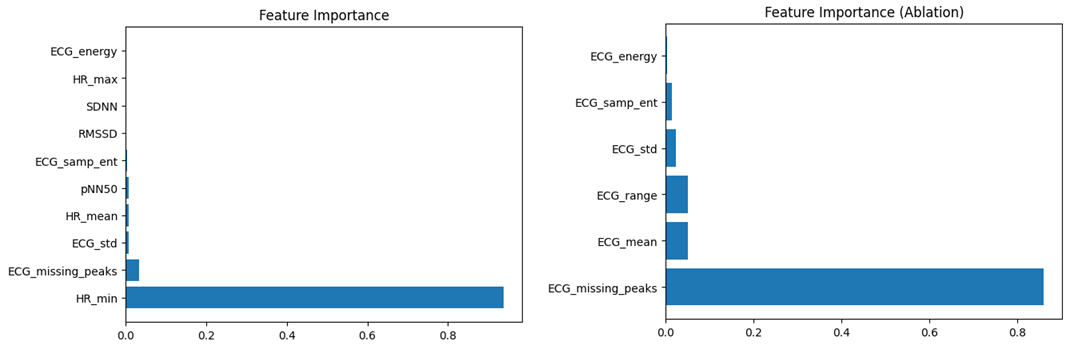
\includegraphics[width=1\textwidth]{ch4/assets/importancefeatureregresion.png}
\caption{Importância das Features na Regressão}
\label{fig:feature_importance}
\end{figure}

Comparação da importância das características no modelo de regressão, considerando todas as features e após a remoção das features derivadas de HR e HRV (\textit{estudo de ablação}). Com todas as features, \texttt{HR\_min} e \texttt{ECG\_missing\_peaks} são as mais determinantes. Após a remoção das features de HR e HRV, outras métricas derivadas do ECG ganham relevância, mas \texttt{ECG\_missing\_peaks} continua a ser a característica principal, evidenciando a sua contribuição crítica para o desempenho do modelo. Em conjunto com os resultados apresentados na tabela, esta análise sugere que as características selecionadas contêm informação suficiente para produzir previsões adequadas do FatigueIndex, mesmo após a remoção das características derivadas de HR e RR.

Os resultados obtidos na regressão indicam que as características utilizadas contêm informação suficiente para modelar o \textit{FatigueIndex}, tanto no cenário original como no \textit{estudo de ablação}, apresentando um desempenho particularmente elevado quando consideradas as observações de um único trabalhador ao longo da sua jornada. No entanto, o objetivo deste trabalho não se limita à estimação do valor numérico do índice, incluindo também a análise da sua representação categórica. Para esse efeito, o \textit{FatigueIndex} foi convertido numa variável categórica através dos percentis P33 e P66, conforme descrito nas secções anteriores, dando origem a três rótulos analíticos definidos para este estudo (LOW, MEDIUM e HIGH). Estes rótulos resultam exclusivamente da discretização do índice construído e não correspondem a níveis clínicos ou a avaliações diretas de fadiga. Assim, torna-se pertinente avaliar se os modelos são igualmente capazes de distinguir entre estas categorias, conduzindo à análise dos modelos de classificação apresentada de seguida.

\clearpage
\paragraph{Métricas do Modelo de Classificação:}
\mbox{}\par
As Tabelas \ref{tab:accuracy_classifier}, \ref{tab:classification_report} e \ref{tab:confusion_matrix} mostram que o desempenho do modelo XGBoost Classifier é praticamente idêntico nos dois cenários. Embora o número de árvores tenha sido ligeiramente reduzido no \textit{estudo de ablação} (de 17 para 14), a \textit{accuracy}, o F1-Score e a distribuição das classificações por classe permanecem inalterados. Estes resultados indicam que o modelo reproduz de forma consistente os rótulos analíticos definidos a partir do \textit{FatigueIndex}, mesmo sem as características derivadas de HR e HRV. As métricas extraídas diretamente do ECG parecem, assim, conter informação suficiente para distinguir as três categorias analíticas utilizadas no estudo, sem que essa distinção constitua uma avaliação clínica ou direta de fadiga.

A Tabela \ref{tab:accuracy_classifier} apresenta os resultados dos modelos de classificação para ambos os cenários.

\par\medskip
\begin{table}[H]
\centering
\caption{Resultados do XGBoost Classifier nos dois cenários de classificação}
\label{tab:accuracy_classifier}
\small
\begin{tabular}{l l c c}
\hline
Modelo & Cenário & Número de Árvores & Accuracy \\
\hline
XGBoost Classifier & Original & 17 & 97.65\% \\
XGBoost Classifier & Estudo de ablação & 14 & 97.65\% \\
\hline
\end{tabular}
\end{table}

A \textit{accuracy} manteve-se em 97,65\% nos dois cenários. A remoção das características derivadas de HR e RR não alterou, portanto, o desempenho global do modelo, apesar da redução do número de árvores de 17 para 14.

A Tabela \ref{tab:classification_report} apresenta o \textit{Classification Report} por classe do XGBoost Classifier.

\begin{table}[H]
\centering
\caption{Classification Report por Classe do XGBoost Classifier}
\label{tab:classification_report}
\small
\begin{tabular}{l c c c c}
\hline
Classe & Precision & Recall & F1-Score & Support \\
\hline
0 & 1.00 & 0.96 & 0.98 & 81 \\
1 & 0.96 & 0.98 & 0.97 & 92 \\
2 & 0.98 & 0.99 & 0.98 & 82 \\
\hline
Accuracy & & & 0.98 & 255 \\
Macro Avg & 0.98 & 0.98 & 0.98 & 255 \\
Weighted Avg & 0.98 & 0.98 & 0.98 & 255 \\
\hline
\end{tabular}
\end{table}

O desempenho por classe é elevado, com valores de F1-Score entre 0,97 e 0,98 e médias macro e ponderada de 0,98. As diferenças entre classes são reduzidas, embora a classe 0 apresente menor \textit{recall} (0,96) e a classe 1 menor \textit{precision} (0,96).

A Tabela \ref{tab:confusion_matrix} apresenta a matriz de confusão.

\begin{table}[H]
\centering
\caption{Matriz de Confusão do XGBoost Classifier nos dois cenários}
\label{tab:confusion_matrix}
\small
\begin{tabular}{c c c c}
\hline
 & Predito 0 & Predito 1 & Predito 2 \\
\hline
Real 0 & 78 & 3 & 0 \\
Real 1 & 0 & 90 & 2 \\
Real 2 & 0 & 1 & 81 \\
\hline
\end{tabular}
\end{table}

A matriz de confusão confirma o elevado desempenho do modelo, uma vez que os erros se concentram apenas entre classes adjacentes. Não se observam confusões diretas entre as classes 0 e 2.

A Figura \ref{fig:feature_importance_classifier} ilustra a importância relativa das features utilizadas no modelo de classificação XGBoost, destacando quais variáveis contribuem mais para as previsões do FatigueIndex.

\begin{figure}[H]
\centering
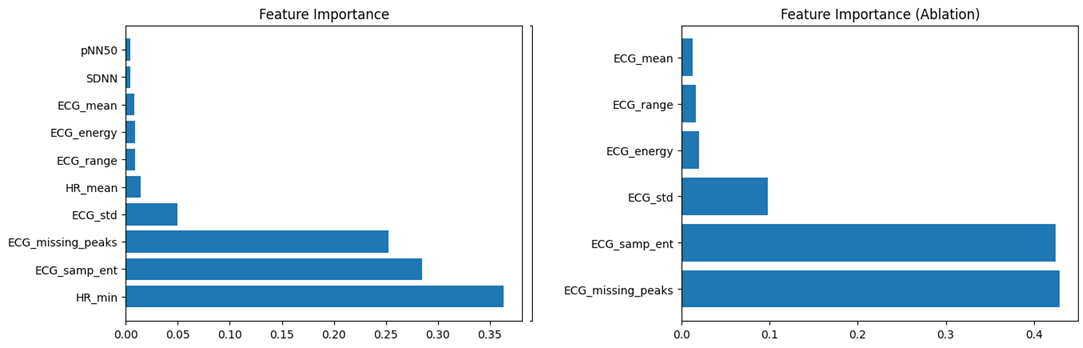
\includegraphics[width=1\textwidth]{ch4/assets/importancefeatureclassifier.png}
\caption{Importância das Features na Classificação}
\label{fig:feature_importance_classifier}
\end{figure}

Comparação da importância das características no modelo XGBoost Classifier, considerando todas as features e após a remoção das features derivadas de HR e RR (\textit{estudo de ablação}). Com todas as features, \texttt{HR\_min} e \texttt{ECG\_missing\_peaks} apresentam a maior relevância na decisão do modelo. Após a remoção das features de HR e RR, outras métricas derivadas do ECG, como \texttt{ECG\_samp\_ent}, ganham importância, mas \texttt{ECG\_missing\_peaks} mantém-se como a característica mais influente, destacando a sua contribuição para a capacidade do modelo em reproduzir corretamente os rótulos analíticos definidos a partir do \textit{FatigueIndex}.

Os resultados obtidos mostram que o XGBoost Classifier é capaz de reproduzir com elevada precisão as categorias analíticas (LOW, MEDIUM e HIGH) definidas a partir do \textit{FatigueIndex}, tanto no cenário original como no \textit{estudo de ablação}. Em conjunto com os resultados da regressão, estes resultados sugerem que as características fisiológicas utilizadas contêm informação suficiente para representar o estado fisiológico codificado pelo índice e permitir a sua estimação, quer como uma variável contínua, quer como uma variável categórica. No entanto, estes resultados foram obtidos considerando as observações de um único trabalhador, pelo que não permitem concluir que os modelos sejam capazes de generalizar para indivíduos diferentes.

Para avaliar esta questão, foi realizada uma experiência adicional na qual os modelos treinados com os dados do trabalhador W01 foram aplicados a outros trabalhadores, nomeadamente W02 e W03. A Tabela \ref{tab:generalizacao_trabalhadores} apresenta os resultados desta análise para a Regressão Linear. Embora o modelo apresente um desempenho praticamente perfeito no próprio W01 ($R^2 = 1.0000$), este resultado não se mantém quando o modelo é aplicado a outros trabalhadores. No W02, o modelo no cenário original explica aproximadamente 32.45\% da variabilidade do \textit{FatigueIndex} ($R^2 = 0.3245$), enquanto no W03 explica apenas 17.33\% ($R^2 = 0.1733$). Estes resultados evidenciam que o elevado desempenho observado no W01 não representa, por si só, uma medida da capacidade de generalização do modelo. Esta limitação é particularmente relevante considerando que o \textit{FatigueIndex} foi construído a partir das próprias características fisiológicas utilizadas como variáveis preditoras. Assim, o modelo pode aprender relações muito específicas entre as características e os padrões fisiológicos de um determinado trabalhador que não se mantêm necessariamente para outros indivíduos.

\begin{table}[H]
\centering
\caption{Desempenho da Regressão Linear treinada com W01 e aplicada a diferentes trabalhadores}
\label{tab:generalizacao_trabalhadores}
\resizebox{\textwidth}{!}{%
\begin{tabular}{l l c c c c}
\hline
Trabalhador & Cenário & MSE & RMSE & MAE & $R^2$ \\
\hline
W01 & Normal, todas as características & 1.3045e-28 & 1.1421e-14 & 5.4600e-15 & 1.0000 \\
W01 & Ablação, sem HR/RR & 0.2659 & 0.5157 & 0.2336 & 0.9699 \\
\hline
W02 & Normal, todas as características & 6.1492 & 2.4798 & 1.6308 & 0.3245 \\
W02 & Ablação, sem HR/RR & 5.0589 & 2.2492 & 1.7092 & 0.4442 \\
\hline
W03 & Normal, todas as características & 9.9222 & 3.1499 & 2.9195 & 0.1733 \\
W03 & Ablação, sem HR/RR & 12.6095 & 3.5510 & 2.9059 & -0.0506 \\
\hline
\end{tabular}
}%
\end{table}

A diferença observada entre trabalhadores pode estar relacionada com a variabilidade individual das respostas fisiológicas, uma vez que valores semelhantes de uma característica podem representar estados fisiológicos distintos em indivíduos diferentes. Fatores como as características individuais, o nível habitual de atividade e as condições de registo dos sinais podem influenciar estas relações. Assim, embora os modelos demonstrem capacidade para aprender uma representação consistente do estado fisiológico codificado pelo índice dentro de um trabalhador, permanece em aberto a sua capacidade de generalizar para indivíduos não observados durante o treino. Esta questão é fundamental para o objetivo do estudo, que pretende desenvolver modelos capazes de estimar indicadores de ativação ou fadiga em diferentes trabalhadores, apesar das diferenças entre os seus padrões fisiológicos. Por este motivo, foram realizadas experiências adicionais com o objetivo de explorar diferentes métodos de treino e modelos que permitissem melhorar a capacidade de generalização entre trabalhadores. Os resultados dessas experiências são apresentados nas secções seguintes.

\subsubsection*{Avaliação para Melhorar a Generalização dos Modelos}

Com o objetivo de melhorar a capacidade de generalização dos modelos entre trabalhadores, foi realizada uma nova experiência utilizando conjuntamente os dados dos trabalhadores W00 a W09. Nesta experiência, foram mantidas as variáveis utilizadas no experimento anterior, mas o processamento foi aplicado de forma padronizada a todos os trabalhadores. A partir do sinal de ECG, foram calculadas as variáveis \texttt{ECG\_mean}, \texttt{ECG\_std}, \texttt{ECG\_range}, \texttt{ECG\_energy}, \texttt{ECG\_samp\_ent} e \texttt{ECG\_missing\_peaks}. A partir dos intervalos RR, foram calculadas as métricas de variabilidade da frequência cardíaca \texttt{SDNN}, \texttt{RMSSD} e \texttt{pNN50}, bem como as variáveis \texttt{HR\_mean}, \texttt{HR\_max} e \texttt{HR\_min}, derivadas da conversão dos intervalos RR em frequência cardíaca. Finalmente, foram criadas as variáveis temporais \texttt{HR\_mean\_ultimos\_5min}, \texttt{cambio\_HR\_vs\_baseline}, \texttt{tendencia\_HR} e \texttt{cambio\_RMSSD}, que representam, respetivamente, a média da frequência cardíaca nas cinco janelas anteriores, a variação da frequência cardíaca relativamente ao \textit{baseline}, a tendência temporal da frequência cardíaca e a variação do RMSSD entre janelas consecutivas.

Os dados foram organizados em janelas consecutivas de 60 segundos. Esta escolha teve dois objetivos principais: reduzir a influência de variações instantâneas, obtendo estimativas mais estáveis das características fisiológicas, e diminuir o impacto dos períodos em que os sinais de HR ou RR não apresentavam valores válidos. Ao aumentar a duração de cada janela, foi possível agregar um maior número de observações e aumentar a probabilidade de obter janelas com todas as características necessárias disponíveis, reduzindo assim a perda de dados durante o processamento. Ao mesmo tempo, a duração de 60 segundos manteve uma resolução temporal suficiente para acompanhar as alterações associadas às diferentes atividades realizadas pelos trabalhadores. Foram também construídas características temporais a partir de janelas anteriores, permitindo representar a evolução dos sinais ao longo do tempo.

Para reduzir o efeito das diferenças fisiológicas entre indivíduos, foi definido um \textit{baseline} individual para cada trabalhador. Foram utilizadas as primeiras 15 janelas completas, correspondentes aproximadamente aos primeiros 15 minutos após a colocação da banda Polar H10 e anteriores ao início da jornada de trabalho. Este período de preparação foi considerado, presumivelmente, uma referência relativamente estável e próxima do estado habitual do trabalhador, sem exposição às exigências da atividade laboral. A partir destas janelas foram calculadas, para cada característica, a média e o desvio padrão individuais, utilizados posteriormente para avaliar as alterações fisiológicas de cada trabalhador.

Esta calibração pode ser comparada ao ajuste de uma balança a zero antes de efetuar uma medição: o sistema estabelece uma referência própria para cada trabalhador, a partir da qual as alterações posteriores podem ser interpretadas. A analogia representa, portanto, a adaptação da medição ao padrão individual, e não a definição de um valor fisiológico universal.

A normalização das características foi realizada através de uma transformação \textit{Z-score} baseada no \textit{baseline} individual, conforme a Equação~\ref{eq:zscore-baseline}:

\begin{equation}
z_{i,f} = \frac{x_{i,f}-\mu_{w,f}}{\sigma_{w,f}}
\label{eq:zscore-baseline}
\end{equation}

onde $x_{i,f}$ corresponde ao valor da característica $f$ na janela $i$, enquanto $\mu_{w,f}$ e $\sigma_{w,f}$ representam, respetivamente, a média e o desvio padrão dessa característica no \textit{baseline} do trabalhador $w$. Assim, um valor $z=0$ corresponde ao comportamento médio do trabalhador, enquanto valores positivos ou negativos representam desvios acima ou abaixo do respetivo estado basal. A normalização foi realizada individualmente para cada trabalhador, não sendo utilizada uma média global.

Esta estratégia permite representar as características em termos de alterações relativas ao estado habitual de cada indivíduo, reduzindo a influência das diferenças interindividuais. Para cada variável original foi criada uma versão normalizada através do \textit{Z-score}, identificada pelo sufixo \texttt{\_z}. Foram estas versões normalizadas que constituíram as entradas dos modelos, permitindo que estes aprendessem padrões associados às variações fisiológicas e não apenas aos valores absolutos característicos de cada trabalhador. O \textit{FatigueIndex} não foi utilizado como entrada, sendo calculado posteriormente a partir das características normalizadas e utilizado exclusivamente como variável objetivo.

O \textit{FatigueIndex} é calculado da mesma forma que na experiência anterior, conforme apresentado no Código~\ref{lst:fatigueindex}, através de uma combinação linear ponderada das mesmas sete variáveis fisiológicas normalizadas. Nesta experiência, essas variáveis foram calculadas relativamente ao \textit{baseline} individual de cada trabalhador, conforme descrito anteriormente.

O índice representa, portanto, uma combinação de desvios fisiológicos relativamente ao \textit{baseline} individual de cada trabalhador. Importa salientar que não corresponde a uma medida clínica direta de fadiga, sendo utilizado neste estudo como uma variável sintética de referência para a definição das categorias do problema de classificação.

Posteriormente, o \textit{FatigueIndex} contínuo foi convertido em três categorias (LOW, MED e HIGH), utilizando os percentis P33 e P66 como limiares. Valores inferiores a P33 foram classificados como LOW, valores entre P33 e P66 como MED e valores iguais ou superiores a P66 como HIGH. Para avaliar a capacidade de generalização entre trabalhadores, foi utilizada a validação cruzada \textit{Leave-One-Subject-Out} (LOSO). Nesta estratégia, cada trabalhador é considerado, de forma sucessiva, como um sujeito independente: em cada iteração, todos os dados de um trabalhador são excluídos do treino e utilizados exclusivamente como conjunto de teste, enquanto os dados dos restantes trabalhadores são utilizados para treinar o modelo. O procedimento é repetido até que todos os trabalhadores tenham sido utilizados uma vez como sujeitos de teste. Para cada iteração, os percentis P33 e P66 foram calculados exclusivamente com os valores do conjunto de treino e posteriormente aplicados ao trabalhador utilizado como teste. Este procedimento evita que a distribuição do trabalhador de teste influencie a definição das categorias e permite avaliar o desempenho do modelo em indivíduos não observados durante o treino, verificando a sua capacidade de generalização para novos trabalhadores, sem que o modelo tenha sido treinado especificamente com os dados desses indivíduos.

O conjunto de dados resultante continha 2,638 janelas, tendo sido atribuída a cada uma delas uma das três categorias do \textit{FatigueIndex}: LOW, MED ou HIGH. A distribuição global das classes foi equilibrada, com 871 observações LOW (33,02\%), 870 observações MED (32,98\%) e 897 observações HIGH (34,00\%). No entanto, o número de observações variou significativamente entre trabalhadores, como apresentado na Tabela \ref{tab:distribuicao_trabalhadores}.

\begin{table}[H]
\centering
\caption{Número de janelas disponíveis por trabalhador.}
\label{tab:distribuicao_trabalhadores}
\tiny
\setlength{\tabcolsep}{2pt}
\resizebox{0.75\textwidth}{!}{%
\begin{tabular}{lrrrrr}
\hline
\textbf{Trabalhador} & \textbf{Janelas} & \textbf{\% do total} & \textbf{LOW} & \textbf{MED} & \textbf{HIGH} \\
\hline
W00 & 104 & 3,9\% & 84 (80,8\%) & 6 (5,8\%) & 14 (13,5\%) \\
W01 & 637 & 24,1\% & 117 (18,4\%) & 270 (42,4\%) & 250 (39,3\%) \\
W02 & 603 & 22,9\% & 106 (17,6\%) & 270 (44,8\%) & 227 (37,7\%) \\
W03 & 407 & 15,4\% & 66 (16,2\%) & 40 (9,8\%) & 301 (74,0\%) \\
W04 & 562 & 21,3\% & 365 (65,0\%) & 179 (31,9\%) & 18 (3,2\%) \\
W05 & 74 & 2,8\% & 21 (28,4\%) & 32 (43,2\%) & 21 (28,4\%) \\
W06 & 35 & 1,3\% & 20 (57,1\%) & 6 (17,1\%) & 9 (25,7\%) \\
W07 & 67 & 2,5\% & 8 (11,9\%) & 16 (23,9\%) & 43 (64,2\%) \\
W08 & 133 & 5,0\% & 79 (59,4\%) & 46 (34,6\%) & 8 (6,0\%) \\
W09 & 16 & 0,6\% & 5 (31,3\%) & 5 (31,3\%) & 6 (37,5\%) \\
\hline
\textbf{Total} & \textbf{2638} & \textbf{100,0\%} & \textbf{871 (33,0\%)} & \textbf{870 (33,0\%)} & \textbf{897 (34,0\%)} \\
\hline
\end{tabular}
}%
\end{table}

Verifica-se que W01, W02 e W04 concentram o maior número de observações, representando, respetivamente, 24,1\%, 22,9\% e 21,3\% do conjunto total. Em contrapartida, W06, W07 e W09 apresentam um número consideravelmente menor de janelas, correspondendo apenas a 1,3\%, 2,5\% e 0,6\% do total, respetivamente. Para além desta assimetria no número de observações, verifica-se também uma distribuição distinta das categorias entre trabalhadores. Por exemplo, a classe HIGH representa 74,0\% das observações de W03, enquanto a classe LOW corresponde a 80,8\% das observações de W00. Estes resultados mostram que, apesar do equilíbrio global entre as três classes, a sua distribuição não é uniforme entre trabalhadores.

Esta variabilidade na quantidade de observações e na distribuição das classes torna necessário avaliar os modelos de forma a garantir que o desempenho obtido não resulta apenas das características dos trabalhadores com maior representação no conjunto de dados. Por esse motivo, os trabalhadores foram separados entre treino e teste, permitindo verificar se os modelos mantêm um desempenho adequado quando aplicados a indivíduos que não participaram no processo de treino.

Outro aspeto relevante deste conjunto de dados corresponde à presença de valores em falta. Foram identificadas 1,732 janelas com pelo menos um valor ausente, correspondendo a 65,66\% do total. A Figura~\ref{fig:rowsmissing} apresenta a distribuição das janelas totais e das janelas com valores em falta por trabalhador. As variáveis de HR e HRV apresentaram a maior proporção de valores em falta, enquanto algumas das características temporais também apresentaram ausência de dados. Estes valores ocorrem principalmente nas janelas iniciais ou em segmentos onde não foi possível calcular determinadas métricas de HRV ou variáveis dependentes de observações anteriores. Para tratar estes valores, foi utilizado o método \texttt{SimpleImputer(strategy='median')}, integrado no \textit{pipeline} do modelo. Assim, em cada \textit{fold}, a mediana de cada variável foi calculada exclusivamente com os dados de treino e utilizada para preencher os valores em falta tanto no treino como no trabalhador reservado para teste. Desta forma, o trabalhador de teste não influencia o cálculo das medianas nem o processo de aprendizagem do modelo.

\begin{figure}[H]
\centering
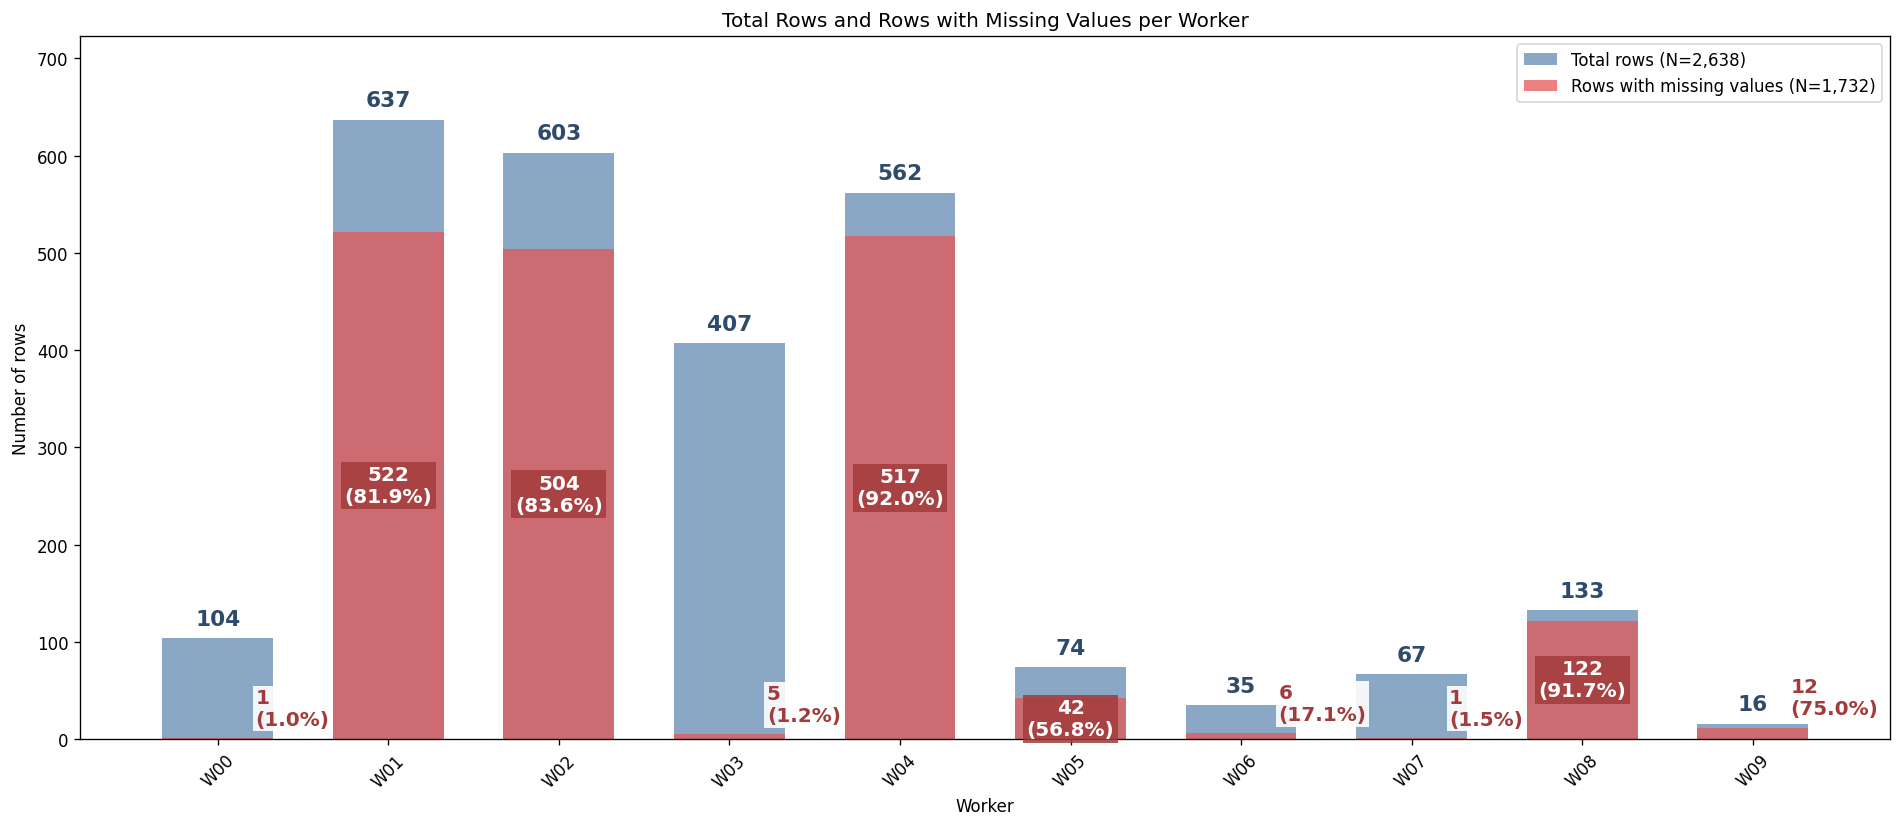
\includegraphics[width=1\textwidth]{ch4/assets/rowsmissing.png}
\caption{Número total de janelas e número de janelas com valores em falta por trabalhador.}
\label{fig:rowsmissing}
\end{figure}

A distribuição apresentada exige uma interpretação cautelosa dos resultados posteriormente obtidos. A disponibilidade desigual dos dados entre trabalhadores pode influenciar o desempenho dos modelos, uma vez que uma quantidade significativa de valores em falta pode comprometer a qualidade das características utilizadas. Estas falhas podem estar associadas, entre outros fatores, à colocação inadequada do dispositivo, a interrupções na transmissão dos dados ou a limitações temporárias na deteção dos sinais fisiológicos. Mesmo nos registos com menor quantidade de dados ausentes, é expectável uma percentagem residual de falhas durante a recolha. Por conseguinte, será necessário verificar, após a avaliação dos modelos, em que medida estas limitações poderão ter condicionado os resultados e confirmar a sua robustez em experiências futuras.

Por sua vez, foram avaliados quatro modelos de classificação: Regressão Logística, Random Forest, SVM e XGBoost. Os modelos receberam como entrada as características fisiológicas e temporais normalizadas e tiveram como objetivo distinguir entre as três categorias de fadiga. A seleção dos hiperparâmetros foi realizada através de validação cruzada interna estratificada no conjunto de treino, sem utilizar informação proveniente do trabalhador reservado para teste.

A avaliação da capacidade de generalização foi realizada através de \textit{Leave-One-Subject-Out Cross-Validation} (LOSO). Em cada iteração, um trabalhador é completamente excluído do treino e utilizado exclusivamente como conjunto de teste, enquanto os restantes trabalhadores são utilizados para treinar o modelo. Neste processo, os limiares P33 e P66, o imputador e os restantes passos de transformação são determinados apenas a partir dos dados de treino, sendo posteriormente aplicados ao trabalhador excluído. O procedimento é repetido até que todos os trabalhadores tenham sido utilizados uma vez como conjunto de teste. Desta forma, a avaliação permite medir diretamente a capacidade do modelo para generalizar para um indivíduo não observado durante o treino.

A Tabela \ref{tab:loso_xgboost_detalhado} apresenta, para o XGBoost, os resultados obtidos em cada uma das dez iterações da avaliação LOSO, permitindo analisar não apenas o desempenho médio do modelo, mas também a variabilidade dos resultados entre trabalhadores.

\begin{table}[H]
\centering
\caption{Validação LOSO do modelo XGBoost Classifier.}
\label{tab:loso_xgboost_detalhado}
\tiny
\resizebox{\textwidth}{!}{%
\begin{tabular}{l l r r r r r r}
\hline
\textbf{Teste} & \textbf{Treino} & \textbf{Recall LOW} & \textbf{Recall MED} & \textbf{Recall HIGH} & \textbf{Accuracy} & \textbf{Balanced Accuracy} & \textbf{Macro-F1} \\
\hline
W00 & W01--W09 & 0,976190 & 0,833333 & 0,785714 & 0,942308 & 0,865079 & 0,854900 \\
W01 & W00, W02--W09 & 0,941748 & 0,921260 & 0,989286 & 0,954474 & 0,950764 & 0,948538 \\
W02 & W00--W01, W03--W09 & 0,895349 & 0,924460 & 0,933054 & 0,923715 & 0,917621 & 0,909651 \\
W03 & W00--W02, W04--W09 & 0,938462 & 0,760000 & 0,977918 & 0,958231 & 0,892127 & 0,903044 \\
W04 & W00--W03, W05--W09 & 0,968421 & 0,911392 & 1,000000 & 0,960854 & 0,959938 & 0,896447 \\
W05 & W00--W04, W06--W09 & 0,857143 & 0,937500 & 0,904762 & 0,905405 & 0,899802 & 0,907857 \\
W06 & W00--W05, W07--W09 & 1,000000 & 0,500000 & 1,000000 & 0,914286 & 0,833333 & 0,855472 \\
W07 & W00--W06, W08--W09 & 0,875000 & 0,250000 & 0,860465 & 0,716418 & 0,661822 & 0,580319 \\
W08 & W00--W07, W09 & 0,614458 & 0,372093 & 0,714286 & 0,541353 & 0,566946 & 0,454266 \\
W09 & W00--W08 & 1,000000 & 1,000000 & 1,000000 & 1,000000 & 1,000000 & 1,000000 \\
\hline
\textbf{Média} & \textit{Média dos folds} & 0,906677 & 0,741004 & 0,916549 & 0,881704 & 0,854743 & 0,831049 \\
\hline
\end{tabular}%
}
\end{table}

Os resultados mostram alguma variabilidade no desempenho do XGBoost consoante o trabalhador utilizado como teste. Globalmente, este foi o modelo que apresentou o melhor desempenho. Nos trabalhadores W01, W02, W03 e W04, o modelo apresenta valores de Accuracy superiores a 0,92, enquanto em W07 e, sobretudo, W08, o desempenho é consideravelmente inferior. No caso de W08, a Accuracy é de 0,54 e o Macro-F1 de 0,45, indicando maior dificuldade em generalizar para este trabalhador. Em contrapartida, o fold correspondente a W09 apresenta desempenho perfeito, embora este resultado deva ser interpretado com cautela devido ao reduzido número de observações deste trabalhador.

De forma global, a média dos dez folds corresponde a uma Accuracy de 0,88, uma Balanced Accuracy de 0,85 e um Macro-F1 de 0,83. O recall foi de 0,91 para LOW, 0,74 para MED e 0,92 para HIGH. Estes resultados mostram que, apesar das diferenças observadas entre trabalhadores, o modelo mantém um desempenho global elevado quando aplicado a indivíduos que não foram utilizados no treino.

As tabelas detalhadas da avaliação LOSO para os modelos Random Forest, SVM e Regressão Logística podem ser consultadas no \textbf{Apêndice~\ref{AppendixC}}. Para facilitar a comparação entre os modelos, a Tabela \ref{tab:loso_classification} apresenta as principais métricas médias obtidas na avaliação LOSO.

\begin{table}[H]
\centering
\caption{Médias globais dos modelos de classificação da avaliação LOSO.}
\label{tab:loso_classification}
\resizebox{\textwidth}{!}{%
\begin{tabular}{lcccccc}
\hline
\textbf{Modelo} & \textbf{Recall LOW} & \textbf{Recall MED} & \textbf{Recall HIGH} & \textbf{Accuracy} & \textbf{Balanced Accuracy} & \textbf{Macro-F1} \\
\hline
XGBoost & 0,91 & 0,74 & 0,92 & 0,88 & 0,85 & 0,83 \\
Random Forest & 0,90 & 0,70 & 0,89 & 0,86 & 0,83 & 0,80 \\
SVM & 0,81 & 0,65 & 0,88 & 0,81 & 0,78 & 0,73 \\
Regressão Logística & 0,87 & 0,66 & 0,69 & 0,78 & 0,74 & 0,70 \\
\hline
\end{tabular}
}%
\end{table}

A comparação entre os modelos mostra que o XGBoost apresenta o melhor desempenho global, com os valores mais elevados de Accuracy (0,88), Balanced Accuracy (0,85) e Macro-F1 (0,83). O Random Forest apresenta resultados próximos, com uma Accuracy de 0,86, uma Balanced Accuracy de 0,83 e um Macro-F1 de 0,80. O SVM apresenta um desempenho inferior, com uma Accuracy de 0,81 e um Macro-F1 de 0,73. Por sua vez, a Regressão Logística obtém os valores mais baixos, com uma Accuracy de 0,78 e um Macro-F1 de 0,70.

A análise do recall mostra ainda que o XGBoost apresenta os melhores resultados nas três categorias, com valores de 0,91 para LOW, 0,74 para MED e 0,92 para HIGH. A classe MED apresenta o menor recall nos quatro modelos, indicando uma maior dificuldade na sua identificação. No caso da Regressão Logística, observa-se também uma redução mais acentuada no desempenho da classe HIGH, com um recall de 0,69.

Para aprofundar a análise do modelo com melhor desempenho, a Tabela \ref{tab:classification_report_xgboost_loso} apresenta o \textit{Classification Report} agregado do XGBoost na avaliação LOSO, incluindo o número de observações, o recall e a precisão obtidos para cada classe.

\begin{table}[H]
\centering
\caption{Classification Report por Classe do XGBoost na avaliação LOSO.}
\label{tab:classification_report_xgboost_loso}
\begin{tabular}{l c c c}
\hline
\textbf{Classe} & \textbf{Support} & \textbf{Recall} & \textbf{Precision} \\
\hline
LOW & 950 & 0,924 & 0,940 \\
MED & 744 & 0,867 & 0,874 \\
HIGH & 944 & 0,959 & 0,937 \\
\hline
\end{tabular}
\end{table}

Neste contexto, o \textit{recall} indica a proporção de observações reais de cada classe que foi corretamente identificada, enquanto a \textit{precision} indica a proporção de previsões de uma classe que estava correta. As tabelas de classificação detalhadas dos restantes modelos podem ser consultadas no \textbf{Apêndice~\ref{AppendixC}}.

Os resultados do \textit{Classification Report} mostram que o XGBoost apresenta um desempenho elevado nas três categorias. A classe HIGH apresenta o maior recall (0,959), seguida da classe LOW (0,924) e da classe MED (0,867). A precisão apresenta valores igualmente elevados, variando entre 0,874 e 0,940. Estes resultados indicam que o modelo consegue identificar de forma consistente as três categorias, embora a classe MED continue a apresentar um desempenho ligeiramente inferior às restantes.

Para analisar de forma mais detalhada os erros cometidos pelo modelo com melhor desempenho, foi construída a matriz de confusão agregada dos dez folds da avaliação LOSO para o XGBoost, apresentada na Tabela \ref{tab:matriz_confusao_agregada_loso}. As matrizes de confusão dos restantes modelos podem ser consultadas no \textbf{Apêndice~\ref{AppendixC}}.

\begin{table}[H]
\centering
\caption{Matriz de Confusão Agregada dos Dez Folds da avaliação LOSO.}
\label{tab:matriz_confusao_agregada_loso}
\begin{tabular}{l c c c}
\hline
 & \textbf{Low} & \textbf{Medium} & \textbf{High} \\
\hline
\textbf{Low} & 878 & 63 & 9 \\
\textbf{Medium} & 47 & 645 & 52 \\
\textbf{High} & 9 & 30 & 905 \\
\hline
\end{tabular}
\end{table}

A matriz de confusão mostra que a maioria das observações foi corretamente classificada pelo XGBoost. Das observações pertencentes à classe LOW, 878 foram corretamente identificadas, enquanto 63 foram classificadas como MED e 9 como HIGH. Para a classe MED, 645 observações foram corretamente classificadas, verificando-se 47 classificações como LOW e 52 como HIGH. Na classe HIGH, 905 observações foram corretamente identificadas, enquanto 9 foram classificadas como LOW e 30 como MED.

Os erros observados concentram-se sobretudo entre categorias adjacentes, sendo a classe MED a que apresenta maior dificuldade de identificação. Este comportamento é consistente com o menor recall obtido para esta categoria, uma vez que uma parte relevante das observações MED é classificada como LOW ou HIGH. Em contrapartida, as classes LOW e HIGH apresentam um número reduzido de classificações entre si, sugerindo que o modelo consegue distinguir de forma mais consistente os extremos do \textit{FatigueIndex}.

Em conjunto, estes resultados mostram que a utilização de características normalizadas relativamente ao \textit{baseline} individual, combinada com dados de vários trabalhadores e com uma avaliação LOSO, permite obter uma capacidade de generalização considerável. Apesar da variabilidade observada entre trabalhadores, o XGBoost apresentou o melhor desempenho médio entre os modelos avaliados, mantendo resultados elevados em vários dos trabalhadores utilizados como teste.

Esta abordagem representa uma evolução relativamente às experiências anteriores, nas quais o desempenho elevado era sobretudo observado quando os dados de treino e teste pertenciam ao mesmo trabalhador. Ao utilizar uma referência fisiológica individual e ao separar completamente os trabalhadores entre treino e teste, a avaliação aproxima-se mais das condições de aplicação pretendidas, nas quais o modelo deverá ser capaz de identificar os diferentes níveis do \textit{FatigueIndex} em trabalhadores não observados durante o treino. Neste contexto, o XGBoost surge como o modelo com maior potencial para as análises desenvolvidas nas experiências seguintes.

\subsubsection*{Testes de Ablação dos Modelos Otimizados para Generalização}

Após a análise da capacidade de generalização dos modelos, foi realizado um \textit{estudo de ablação} para avaliar o contributo dos diferentes grupos de características para o desempenho da classificação. Foram consideradas características derivadas do ECG, de HR e dos intervalos R-R, bem como variáveis temporais delas derivadas, procurando determinar se seria possível reduzir o conjunto de entradas sem comprometer significativamente a capacidade de generalização.

Esta análise apresenta também interesse do ponto de vista prático, uma vez que as características derivadas de HR e R-R apresentam, em determinadas janelas, uma maior presença de valores em falta, devido às próprias características do processo de aquisição e cálculo destas medidas. Além disso, a sua utilização pode estar associada a limitações na deteção das medidas em determinadas condições de registo. Neste contexto, avaliar o impacto da sua remoção permite determinar se as características derivadas do ECG conseguem fornecer informação suficiente para manter um desempenho adequado, reduzindo simultaneamente a dependência de variáveis com maior ocorrência de valores em falta.

Para esta análise foram considerados três cenários experimentais. O cenário A, já apresentado na secção anterior, corresponde à utilização de todas as características. No cenário B, foram removidas as características derivadas diretamente do ECG, mantendo-se apenas as características de HR/R-R e temporais. No cenário C, foram removidas as características de HR/R-R e temporais, sendo utilizadas exclusivamente as características derivadas do ECG.

Em todos os cenários, foram mantidas as condições de avaliação utilizadas anteriormente, nomeadamente a validação \textit{Leave-One-Subject-Out Cross-Validation} (LOSO). Em cada iteração, um trabalhador foi reservado exclusivamente para teste, enquanto os restantes foram utilizados no treino. A definição das categorias, a imputação dos valores em falta e os restantes passos de transformação foram realizados sem utilizar informação do trabalhador de teste. Desta forma, foi possível comparar os diferentes conjuntos de características nas mesmas condições e avaliar simultaneamente a sua contribuição para a classificação e a capacidade de generalização para trabalhadores não observados durante o treino.

Os resultados dos cenários B e C são comparados com o cenário A, utilizado como referência, na Tabela \ref{tab:ablation_comparacao}. Desta forma, a análise centra-se no impacto da remoção de diferentes grupos de características.

\begin{table}[H]
\centering
\caption{Comparação do desempenho dos modelos nos três cenários do estudo de ablação, com avaliação LOSO.}
\label{tab:ablation_comparacao}
\resizebox{\textwidth}{!}{%
\begin{tabular}{llccc}
\hline
\textbf{Modelo} & \textbf{Cenário} & \textbf{Accuracy} & \textbf{Balanced Accuracy} & \textbf{Macro-F1} \\
\hline
Regressão Logística & A: Todas as características & 0,7817 & 0,7426 & 0,7007 \\
Regressão Logística & B: HR/R-R + temporais & 0,5647 & 0,5309 & 0,4709 \\
Regressão Logística & C: ECG & 0,5974 & 0,5369 & 0,5012 \\
\hline
Random Forest & A: Todas as características & 0,8616 & 0,8291 & 0,8039 \\
Random Forest & B: HR/R-R + temporais & 0,6619 & 0,6436 & 0,6045 \\
Random Forest & C: ECG & 0,6636 & 0,6073 & 0,5728 \\
\hline
SVM & A: Todas as características & 0,8055 & 0,7799 & 0,7311 \\
SVM & B: HR/R-R + temporais & 0,6210 & 0,6213 & 0,5569 \\
SVM & C: ECG & 0,6133 & 0,5749 & 0,5296 \\
\hline
XGBoost & A: Todas as características & 0,8817 & 0,8547 & 0,8310 \\
XGBoost & B: HR/R-R + temporais & 0,6566 & 0,6413 & 0,5991 \\
XGBoost & C: ECG & 0,6783 & 0,6136 & 0,5892 \\
\hline
\end{tabular}%
}
\end{table}

A comparação entre os três cenários evidencia uma perda de desempenho quando parte das características é removida. Em todos os modelos, o cenário A, que combina as características de ECG, HR/R-R e temporais, apresenta os melhores resultados, confirmando o contributo complementar destas fontes de informação. No XGBoost, o cenário A produz uma Accuracy de 0,8817, uma Balanced Accuracy de 0,8547 e um Macro-F1 de 0,8310; no cenário B, baseado apenas em HR/R-R e variáveis temporais, estes valores descem para 0,6566, 0,6413 e 0,5991, respetivamente. Esta redução mostra que esse subconjunto não preserva o desempenho obtido com a combinação completa das variáveis.

No cenário C, baseado exclusivamente nas características derivadas do ECG, o XGBoost obtém uma Accuracy de 0,6783, uma Balanced Accuracy de 0,6136 e um Macro-F1 de 0,5892. Embora o ECG permita recuperar ligeiramente a Accuracy face ao cenário B, os valores inferiores de Balanced Accuracy e Macro-F1 mostram que essa vantagem não se distribui uniformemente pelas classes, mantendo-se os resultados claramente abaixo do cenário A. Os restantes modelos seguem a mesma tendência: no Random Forest, as Accuracies dos cenários B e C são semelhantes (0,6619 e 0,6636), mas o cenário B apresenta melhor Balanced Accuracy (0,6436 contra 0,6073) e Macro-F1 (0,6045 contra 0,5728); no SVM, a Accuracy diminui de 0,8055 no cenário A para 0,6210 no cenário B e 0,6133 no cenário C; e, na Regressão Logística, diminui de 0,7817 para 0,5647 e 0,5974, respetivamente. 

A Figura \ref{fig:ablation_feature_importance_xgboost} apresenta a importância relativa das características utilizadas pelo XGBoost nos três cenários do estudo de ablação.

\begin{figure}[H]
\centering
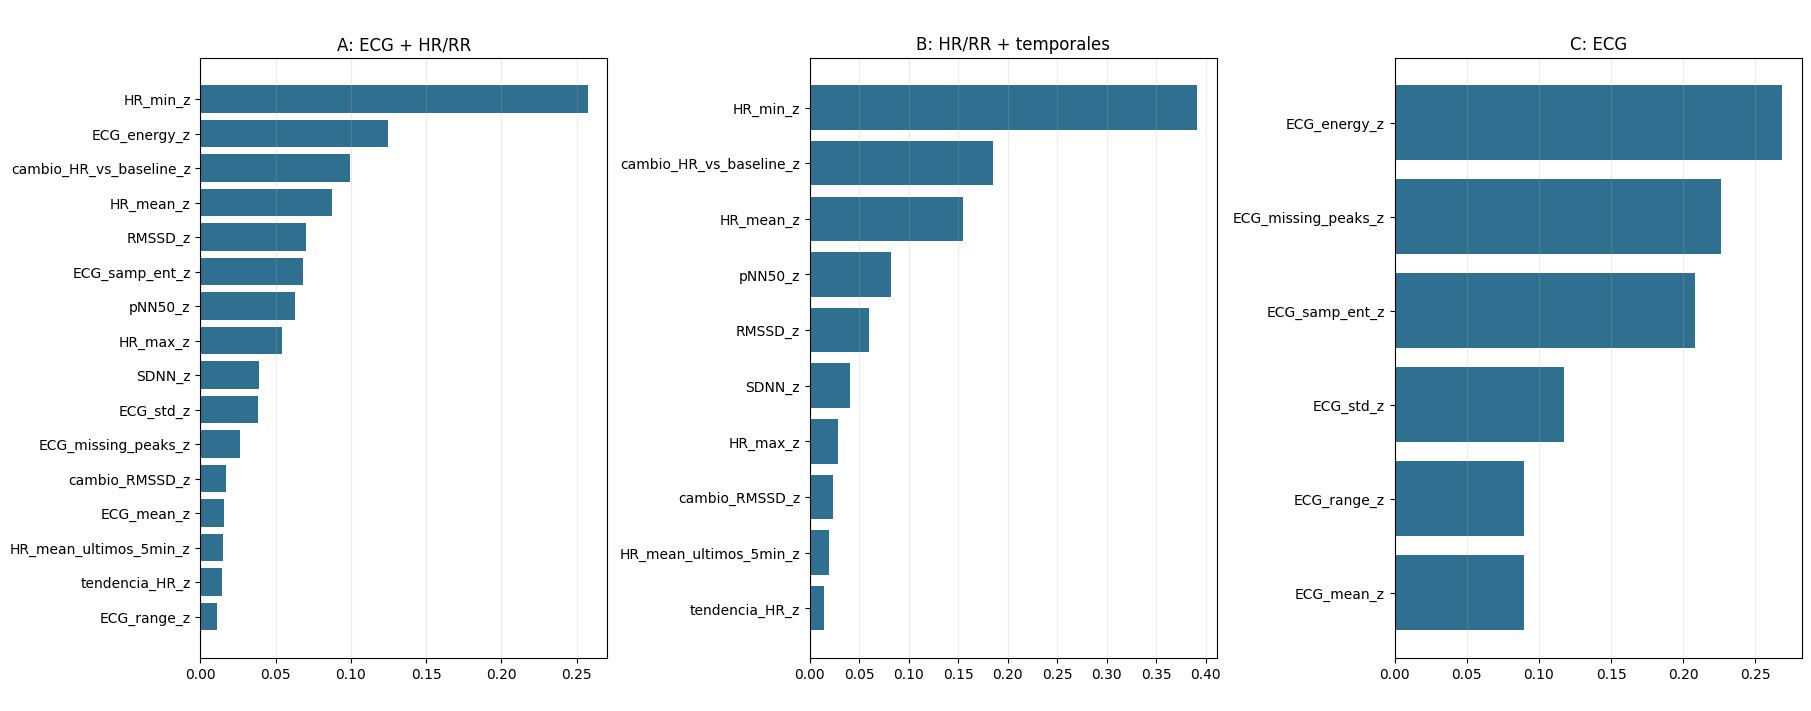
\includegraphics[width=1\textwidth]{ch4/assets/importanceXGBOST.png}
\caption{Importância relativa das características no XGBoost nos três cenários do estudo de ablação.}
\label{fig:ablation_feature_importance_xgboost}
\end{figure}

\begin{sloppypar}
No cenário A, com todas as características, destacam-se \texttt{HR\_min\_z}, \texttt{ECG\_energy\_z} e \texttt{cambio\_HR\_vs\_baseline\_z}. No cenário B, sem características de ECG, \texttt{HR\_min\_z} e \texttt{cambio\_HR\_vs\_baseline\_z} mantêm-se entre as mais relevantes. No cenário C, sem características de HR/R-R e temporais, \texttt{ECG\_energy\_z} continua a ser a mais importante. Assim, embora a distribuição seja menos equilibrada, a hierarquia das características mantém alguma semelhança com o cenário completo. As figuras dos restantes modelos são apresentadas no \textbf{Apêndice~\ref{AppendixD}}.
\end{sloppypar}

Estes resultados mostram que, no contexto da generalização entre trabalhadores, a remoção de uma das fontes de informação provoca uma perda de desempenho relevante. Embora as características derivadas do ECG mantenham capacidade discriminativa quando utilizadas isoladamente, os resultados obtidos no cenário C indicam que estas não são suficientes para atingir o desempenho alcançado pela combinação das diferentes fontes. Por outro lado, a manutenção das características de HR/R-R e temporais sem as características de ECG também não permite preservar o desempenho observado no cenário completo.

A análise permite ainda estabelecer uma comparação com o estudo realizado anteriormente para um único trabalhador. Nesse cenário, a remoção das características de HR/R-R permitia manter um desempenho relativamente elevado utilizando so características derivadas do ECG. No entanto, os resultados obtidos com a avaliação LOSO mostram que esta capacidade não se mantém no mesmo nível quando o modelo é aplicado a trabalhadores não observados durante o treino. Assim, o desempenho anteriormente observado com um único trabalhador não pode ser diretamente generalizado para o cenário inter-trabalhador.

De forma geral, a combinação de características de ECG, HR/R-R e variáveis temporais revelou-se a abordagem mais adequada para generalizar a classificação entre trabalhadores. Embora as características de ECG mantenham capacidade discriminativa isoladamente, a sua utilização, tal como a utilização exclusiva de HR/R-R e variáveis temporais, implica uma perda significativa de desempenho. Entre os modelos avaliados, o XGBoost apresentou os melhores resultados nos três cenários, reforçando a importância de integrar diferentes fontes de informação fisiológica para classificar os níveis definidos pelo \textit{FatigueIndex} em trabalhadores não observados durante o treino.

\subsubsection*{Validação Externa com Dados Experimentais do Polar H10}

Após a avaliação da capacidade de generalização dos modelos através de LOSO e do \textit{estudo de ablação}, foi realizada uma experiência adicional com o objetivo de observar o comportamento temporal dos modelos quando aplicados a um novo participante. Para esta análise foram utilizados os dados de um participante cujos dados não foram utilizados no treino dos modelos. Foram analisados dois registos correspondentes a condições experimentais distintas: um registo realizado durante \textbf{exercício e atividade física} e outro registo realizado durante \textbf{trabalho no computador}.

Nesta experiência foram utilizados os quatro modelos globais anteriormente treinados (Regressão Logística, Random Forest, SVM e XGBoost), utilizando o conjunto completo de características disponível, composto por variáveis derivadas do ECG, características relacionadas com HR e intervalos R-R e variáveis temporais. Os dados do Polar H10 foram submetidos ao mesmo pré-processamento e às mesmas etapas de \textit{feature engineering} utilizadas durante o treino, incluindo a extração das características e a organização dos dados em janelas consecutivas de 60 segundos. Os modelos foram carregados a partir dos ficheiros previamente guardados e aplicados diretamente aos dados processados.

Como os registos não possuíam etiquetas previamente atribuídas, a atividade realizada foi utilizada como referência contextual para interpretar as previsões. No registo de exercício e atividade física, esperavam-se estados de maior ativação fisiológica, enquanto no registo de trabalho no computador se esperavam estados associados a uma menor intensidade física. A análise procurou ainda verificar se as previsões apresentavam uma evolução temporal coerente ao longo das janelas consecutivas.

A Tabela \ref{tab:polar_h10_datasets} apresenta o número de janelas analisadas e a duração aproximada de cada registo.

\begin{table}[H]
\centering
\caption{Conjuntos de dados analisados no novo participante.}
\label{tab:polar_h10_datasets}
\small
\begin{tabular*}{0.8\textwidth}{@{\extracolsep{\fill}}l c c c@{}}
\toprule
\textbf{Registo} & \textbf{Nº de janelas} & \textbf{Duração aproximada} & \textbf{Intervalo temporal} \\
\midrule
\texttt{PC} & 153 & 2~h~32~min & \texttt{2:01 PM--4:33 PM} \\
\texttt{EXERCISE} & 119 & 1~h~58~min & \texttt{7:40 PM--9:38 PM} \\
\bottomrule
\end{tabular*}
\end{table}

O registo de exercício e atividade física foi dividido em dois períodos experimentais, correspondentes à caminhada na passadeira e ao trote. A Tabela~\ref{tab:polar_exercise_periods} apresenta os intervalos temporais e o número de janelas considerados em cada período.

\begin{table}[H]
\centering
\caption{Divisão temporal do registo de exercício e atividade física.}
\label{tab:polar_exercise_periods}
\small
\begin{tabular*}{0.8\textwidth}{@{\extracolsep{\fill}}l c c c@{}}
\hline
\textbf{Registo} & \textbf{Nº de janelas} & \textbf{Duração aproximada} & \textbf{Intervalo temporal} \\
\hline
\texttt{CAMINHADA} & 40 & 20~min & \texttt{9:05 PM--9:25 PM} \\
\texttt{TROTE} & 20 & 10~min & \texttt{9:25 PM--9:35 PM} \\
\hline
\end{tabular*}
\end{table}

As Figuras~\ref{fig:polar_predictions_pc} e~\ref{fig:polar_predictions_exercise} apresentam as previsões dos quatro modelos para os registos de trabalho no computador e de exercício e atividade física, respetivamente. Em cada gráfico, as classes Baixa, Média e Alta correspondem às categorias previstas pelos modelos ao longo das janelas temporais de 60 segundos.

\begin{figure}[H]
\centering
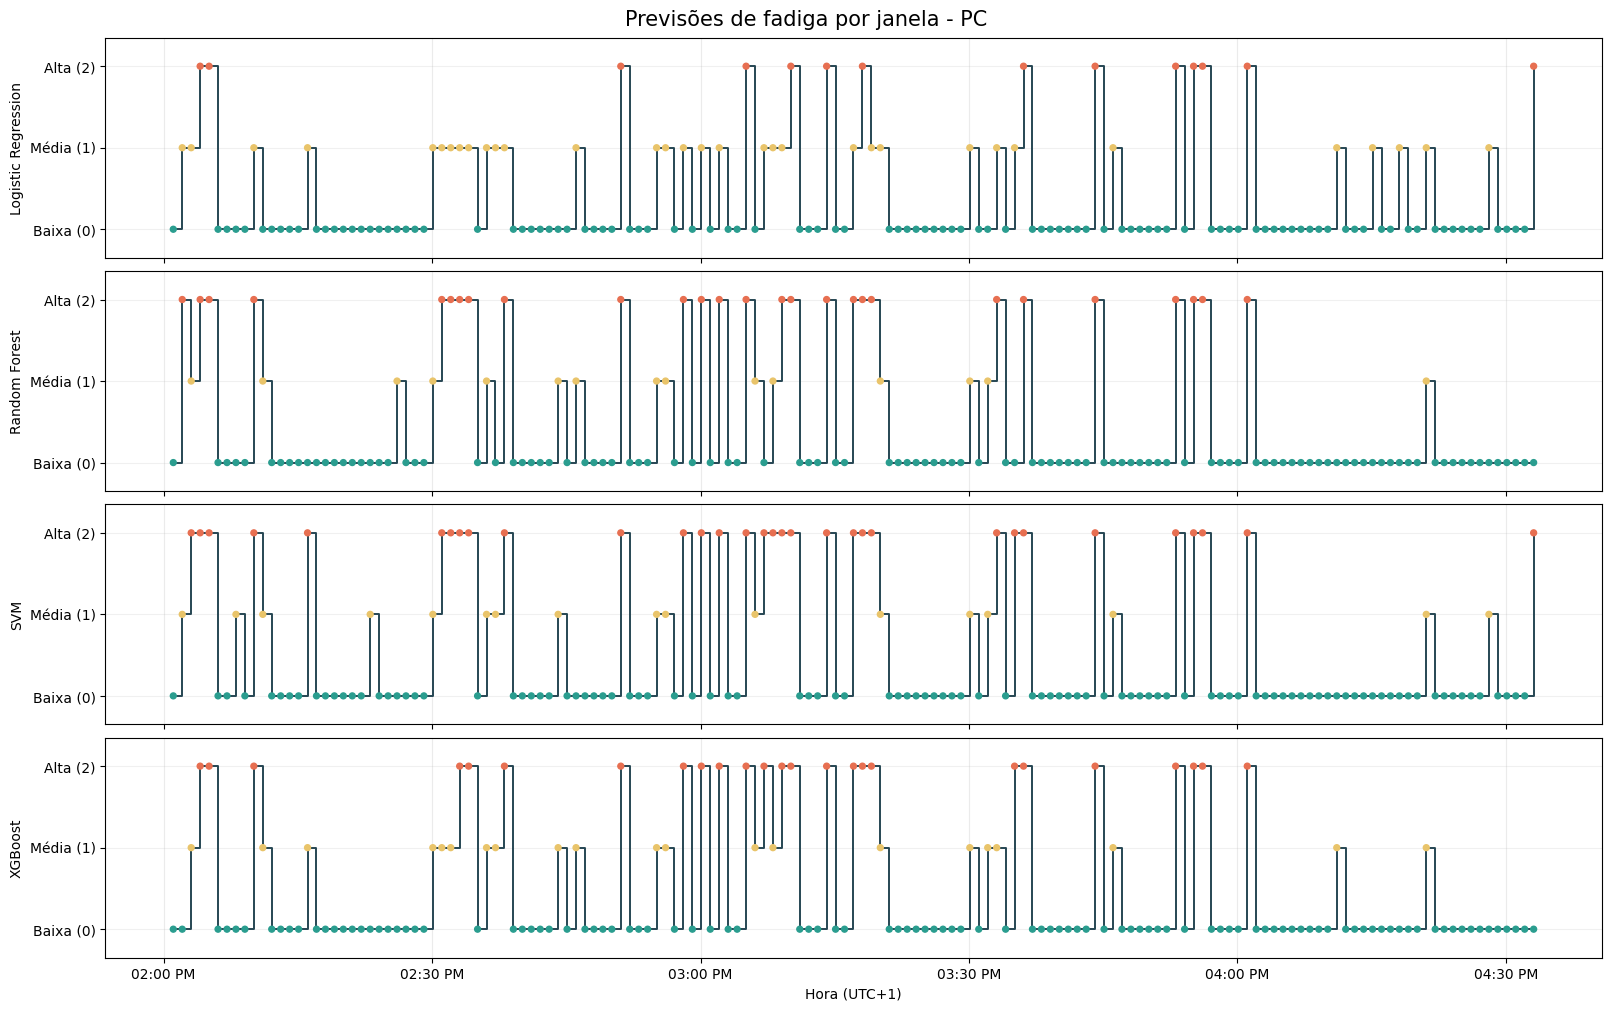
\includegraphics[width=\textwidth]{ch4/assets/prediccionesPCPOLAR.png}
\caption{Previsões dos modelos para o registo de trabalho no computador com dados do Polar H10.}
\label{fig:polar_predictions_pc}
\end{figure}

\begin{figure}[H]
\centering
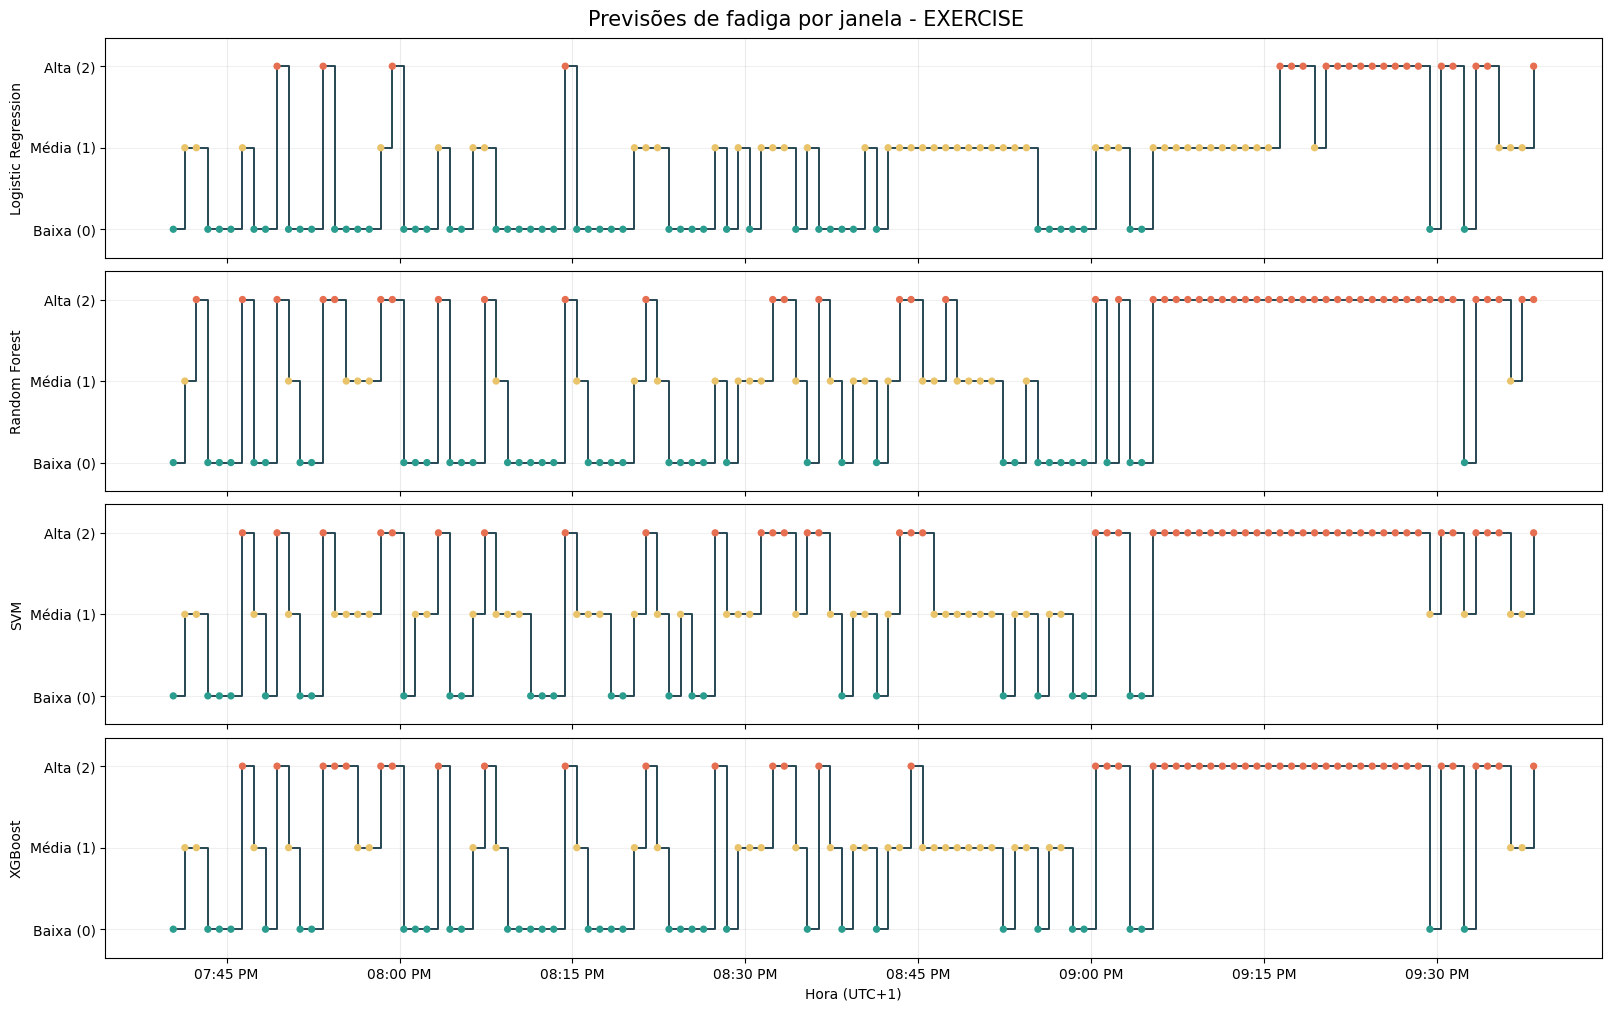
\includegraphics[width=\textwidth]{ch4/assets/prediccionesEJERCICEPOLAR.png}
\caption{Previsões dos modelos para o registo de exercício e atividade física com dados do Polar H10.}
\label{fig:polar_predictions_exercise}
\end{figure}

Para complementar esta análise, a Tabela~\ref{tab:polar_predictions_summary} apresenta o número de janelas classificadas como LOW, MED e HIGH por cada modelo em cada condição experimental.

\begin{table}[H]
\centering
\footnotesize
\caption{Distribuição das classes previstas pelos modelos nas duas condições experimentais.}
\label{tab:polar_predictions_summary}
\resizebox{0.8\textwidth}{!}{%
\begin{tabular}{l l c c c}
\hline
\textbf{Registo} & \textbf{Modelo} & \textbf{LOW} & \textbf{MED} & \textbf{HIGH} \\
\hline
Trabalho no computador & Regressão Logística & 106 & 33 & 14 \\
Trabalho no computador & Random Forest & 111 & 15 & 27 \\
Trabalho no computador & SVM & 104 & 17 & 32 \\

Trabalho no computador & XGBoost & 107 & 21 & 25 \\
\hline
Exercício e atividade física & Regressão Logística & 50 & 48 & 21 \\
Exercício e atividade física & Random Forest & 42 & 26 & 51 \\
Exercício e atividade física & SVM & 26 & 42 & 51 \\
Exercício e atividade física & XGBoost & 37 & 33 & 49 \\
\hline
\end{tabular}%
}
\end{table}

No registo de trabalho no computador (\texttt{PC}), verifica-se uma predominância clara da classe LOW em todos os modelos, com valores entre 104 e 111 janelas. A Regressão Logística apresenta o menor número de previsões HIGH, com 14 janelas (9,15\%), enquanto o SVM apresenta o maior, com 32 janelas (20,92\%). Os restantes modelos apresentam valores intermédios. Esta tendência é igualmente visível na Figura~\ref{fig:polar_predictions_pc}, onde as previsões HIGH surgem de forma pontual e intercalada com períodos de LOW e MED.

No registo de exercício e atividade física (\texttt{EXERCISE}), observa-se uma distribuição diferente das classes. Verifica-se um aumento das previsões MED e HIGH, sobretudo nos modelos Random Forest, SVM e XGBoost, que apresentam, respetivamente, 51, 51 e 49 janelas classificadas como HIGH. A Regressão Logística apresenta um comportamento mais conservador, com 50 janelas LOW, 48 MED e 21 HIGH. Esta diferença em relação ao registo \texttt{PC} é igualmente evidente na Figura~\ref{fig:polar_predictions_exercise}, onde se observam períodos prolongados de previsões HIGH, particularmente na parte final do registo.

Para complementar esta análise, foi definido um critério contextual baseado na atividade realizada durante cada registo. Foram considerados quatro casos: o conjunto \texttt{PC} completo, o conjunto \texttt{EXERCISE} completo, o intervalo de caminhada na passadeira e o intervalo de trote. No conjunto \texttt{PC}, foram consideradas compatíveis com o contexto as previsões LOW e MED. No conjunto \texttt{EXERCISE} completo, foram consideradas compatíveis as previsões MED e HIGH. Nos intervalos específicos, foram consideradas compatíveis as previsões MED e HIGH durante a caminhada em passadeira, enquanto durante o trote foi considerada compatível apenas a classe HIGH. A Tabela~\ref{tab:polar_full_context_agreement} apresenta os resultados dos dois registos completos, e a Tabela~\ref{tab:polar_context_agreement} apresenta os resultados dos dois intervalos de exercício.

\begin{table}[H]
\centering
\footnotesize
\caption{Concordância das previsões com o contexto nos registos completos PC e EXERCISE.}
\label{tab:polar_full_context_agreement}
\setlength{\tabcolsep}{1pt}
\begin{tabular*}{\textwidth}{@{\extracolsep{\fill}}l l c c c c c@{}}
\hline
\textbf{Registo} & \textbf{Modelo} & \shortstack{\textbf{Janelas}\\\textbf{totais}} & \shortstack{\textbf{Janelas}\\\textbf{compatíveis}} & \shortstack{\textbf{Janelas não}\\\textbf{compatíveis}} & \shortstack{\textbf{\%}\\\textbf{compatível}} & \shortstack{\textbf{\% não}\\\textbf{compatível}} \\
\hline
\textbf{PC} & Regressão Logística & 153 & 139 & 14 & 90,85 & 9,15 \\
\textbf{PC} & Random Forest & 153 & 126 & 27 & 82,35 & 17,65 \\
\textbf{PC} & SVM & 153 & 121 & 32 & 79,08 & 20,92 \\
\textbf{PC} & XGBoost & 153 & 128 & 25 & 83,66 & 16,34 \\
\hline
\textbf{EXERCISE} & Regressão Logística & 119 & 69 & 50 & 57,98 & 42,02 \\
\textbf{EXERCISE} & Random Forest & 119 & 77 & 42 & 64,71 & 35,29 \\
\textbf{EXERCISE} & SVM & 119 & 93 & 26 & 78,15 & 21,85 \\
\textbf{EXERCISE} & XGBoost & 119 & 82 & 37 & 68,91 & 31,09 \\
\hline
\end{tabular*}
\end{table}

No registo completo de trabalho no computador (\texttt{PC}), a Regressão Logística apresenta a maior concordância com o contexto, com 139 de 153 janelas compatíveis (90,85\%). O SVM apresenta o valor mais baixo, com 121 janelas compatíveis (79,08\%), enquanto o Random Forest e o XGBoost apresentam valores intermédios de concordância.

No registo completo de exercício e atividade física (\texttt{EXERCISE}), a concordância é inferior à observada no conjunto \texttt{PC} para a maioria dos modelos. O SVM apresenta o melhor resultado, com 93 de 119 janelas compatíveis (78,15\%), enquanto a Regressão Logística apresenta o valor mais baixo, com 69 janelas compatíveis (57,98\%). O Random Forest e o XGBoost apresentam valores intermédios.

\begin{table}[H]
\centering
\caption{Concordância das previsões com o contexto nos intervalos de caminhada e trote.}
\label{tab:polar_context_agreement}
\footnotesize
\setlength{\tabcolsep}{1pt}
\begin{tabular*}{\textwidth}{@{\extracolsep{\fill}}l l c c c c c@{}}
\hline
\textbf{Registo} & \textbf{Modelo} & \shortstack{\textbf{Janelas}\\\textbf{totais}} & \shortstack{\textbf{Janelas}\\\textbf{compatíveis}} & \shortstack{\textbf{Janelas não}\\\textbf{compatíveis}} & \shortstack{\textbf{\%}\\\textbf{compatível}} & \shortstack{\textbf{\% não}\\\textbf{compatível}} \\
\hline
\textbf{CAMINHADA} & Regressão Logística & 20 & 20 & 0 & 100,0 & 0,0 \\
\textbf{CAMINHADA} & Random Forest & 20 & 20 & 0 & 100,0 & 0,0 \\
\textbf{CAMINHADA} & SVM & 20 & 20 & 0 & 100,0 & 0,0 \\
\textbf{CAMINHADA} & XGBoost & 20 & 20 & 0 & 100,0 & 0,0 \\
\hline
\textbf{TROTE} & Regressão Logística & 10 & 8 & 2 & 80,0 & 20,0 \\
\textbf{TROTE} & Random Forest & 10 & 9 & 1 & 90,0 & 10,0 \\
\textbf{TROTE} & SVM & 10 & 8 & 2 & 80,0 & 20,0 \\
\textbf{TROTE} & XGBoost & 10 & 8 & 2 & 80,0 & 20,0 \\
\hline
\end{tabular*}
\end{table}

Durante a caminhada em passadeira, os quatro modelos apresentam concordância total com o critério contextual definido, classificando todas as 20 janelas como MED ou HIGH. Este resultado corresponde a 100,0\% de janelas compatíveis para todos os modelos. 

Durante o trote, observa-se uma pequena redução dessa concordância. O Random Forest apresenta 9 de 10 janelas compatíveis (90,0\%), enquanto a Regressão Logística, o SVM e o XGBoost apresentam 8 de 10 janelas compatíveis (80,0\%). Assim, o Random Forest apresenta a maior concordância com o critério contextual nesta fase do exercício.

Embora a Regressão Logística não apresente o melhor resultado em todas as análises, as suas previsões revelam um comportamento mais conservador na atribuição da classe HIGH. Em comparação com os restantes modelos, tende a produzir mais previsões MED e menos previsões HIGH, o que pode ser vantajoso por reduzir a ocorrência de alertas excessivos ou a identificação de uma intensidade elevada durante atividades moderadas. Esta diferença é particularmente evidente durante a caminhada na passadeira, entre as 9:05 PM e as 9:25 PM, período em que a Regressão Logística foi o único modelo a classificar todas as janelas como MED, enquanto os restantes modelos atribuíram a maioria dessas janelas à classe HIGH. Considerando que este intervalo correspondia a exercício, mas não a uma situação de esforço máximo, este comportamento parece mais coerente com a intensidade esperada da atividade. Durante o trote, entre as 9:25 PM e as 9:35 PM, a Regressão Logística passou a atribuir a classe HIGH, acompanhando o comportamento geral dos restantes modelos perante uma atividade mais intensa.

Apesar destes resultados, o critério utilizado é apenas contextual e não constitui uma etiqueta independente do nível real de fadiga; por isso, as janelas ``compatíveis'' não devem ser interpretadas como classificações verdadeiramente corretas nem como métricas de desempenho. Ainda assim, a experiência mostra que os modelos globais podem produzir previsões em registos contínuos de um novo participante com o Polar H10, revelando predominância de LOW no trabalho no computador, aumento de MED e HIGH durante o exercício e elevada concordância entre os modelos em vários períodos. Desta forma, a análise complementa os resultados de LOSO ao evidenciar o comportamento dos modelos perante diferentes condições experimentais.

\subsubsection*{Resultados das Experiências com o Relógio Empatica EmbracePlus}

Os modelos desenvolvidos com os dados do relógio Empatica EmbracePlus foram avaliados em duas configurações distintas: utilizando os dados originais ao nível do minuto e utilizando dados agregados através de janelas temporais de 10 minutos. Em ambos os cenários foram analisados os algoritmos \textit{Gaussian Mixture Model (GMM)} e \textit{Clustering Hierárquico Aglomerativo}. Adicionalmente, os agrupamentos obtidos foram interpretados através de uma Árvore de Decisão, permitindo avaliar a consistência e a interpretabilidade das fronteiras entre clusters.

\paragraph{Resultados dos Modelos de Clustering}

A Tabela \ref{tab:clustering_metrics} apresenta as principais métricas obtidas para os modelos de clustering.

\begin{table}[H]
\centering
\caption{Métricas Estruturais dos Modelos de Clustering}
\label{tab:clustering_metrics}
\resizebox{\textwidth}{!}{%
\begin{tabular}{l c c c c c}
\hline
Algoritmo & Dados & Original / PCA & Critério de Seleção & Clusters ($k$) & Silhouette Score \\
\hline
GMM & Original & 12 / 6 & BIC & 9 & 0.3475 \\
GMM (Restrito) & Original & 12 / 6 & Heurístico* & 4 & 0.3343 \\
GMM & Janelas (10 min) & 12 / 4 & BIC & 5 & 0.3742 \\
\hline
Clustering Hierárquico & Original & 12 / -- & Silhouette + Elbow & 5 & 0.3959 \\
Clustering Hierárquico & Janelas (10 min) & 12 / -- & Silhouette + Elbow & 5 & 0.4132 \\
\hline
\end{tabular}%
}
\end{table}

\noindent
*Configuração alternativa forçada para limitar o número de estados a um patamar fisiologicamente interpretável, ignorando a recomendação teórica ideal do critério BIC.

Os resultados evidenciam que a aplicação de etapas diferenciadas de engenharia e redução de características influenciou diretamente o desempenho e a estrutura dos agrupamentos obtidos em ambos os algoritmos:

\begin{itemize}
\item \textbf{Impacto do PCA e Dimensões de Entrada:} No modelo Gaussian Mixture Model (GMM), foi aplicada uma etapa de redução da dimensionalidade através de \textit{Principal Component Analysis (PCA)} antes do treino. Esta abordagem permitiu reduzir a complexidade do espaço de características, preservando aproximadamente 90\% da variância original dos dados. Nos dados ao nível do minuto, o PCA resultou em seis componentes principais, enquanto na abordagem baseada em janelas temporais foram obtidas quatro componentes. A redução da dimensionalidade contribuiu para simplificar a modelação probabilística do GMM, reduzindo o número de parâmetros a estimar e tornando o processo de aprendizagem mais estável. Em contraste, o Clustering Hierárquico Aglomerativo foi treinado diretamente sobre as features previamente normalizadas, sem aplicação de PCA, uma vez que o objetivo era preservar as relações de distância entre as variáveis originais utilizadas na construção do dendrograma.

\item \textbf{Impacto do Ventaneamento Temporal (Janelas):} O Silhouette Score foi utilizado para avaliar a qualidade dos agrupamentos obtidos, medindo simultaneamente a coesão interna de cada cluster e a sua separação relativamente aos restantes. Esta métrica assume valores entre $-1$ e $1$, sendo que valores mais próximos de $1$ indicam agrupamentos mais compactos e bem separados, enquanto valores próximos de $0$ sugerem sobreposição entre clusters e valores negativos apontam para classificações inadequadas.

A aplicação de janelas temporais de $10$ minutos permitiu reduzir as flutuações fisiológicas instantâneas e o ruído presente nos sinais, produzindo representações mais estáveis do estado fisiológico dos participantes. Este efeito refletiu-se diretamente nos valores do Silhouette Score, que aumentaram em ambos os algoritmos. No Gaussian Mixture Model (GMM), a métrica evoluiu de $0.3475$ para $0.3742$, enquanto no Clustering Hierárquico Aglomerativo aumentou de $0.3959$ para $0.4132$. Embora o incremento seja moderado, demonstra que a agregação temporal favoreceu a formação de clusters mais consistentes e melhor definidos, facilitando a identificação de padrões fisiológicos representativos de diferentes estados de atividade e repouso.

\item \textbf{Seleção Estrutural dos Clusters GMM ($k$):} No \textit{Gaussian Mixture Model (GMM)}, o critério \textit{Bayesian Information Criterion (BIC)} indicou como solução ótima a utilização de nove clusters para os dados ao nível do minuto e cinco clusters para os dados agregados em janelas de 10 minutos, conforme ilustrado graficamente na Figura \ref{fig:bic_curves}. Apesar de apresentar o melhor compromisso entre qualidade de ajuste e complexidade do modelo, a solução com nove clusters revelou-se excessivamente fragmentada para uma interpretação fisiológica intuitiva. Por esse motivo, foi realizada uma experiência adicional, restringindo o modelo a \textit{$k=4$} clusters (\textit{GMM Restrito}), mantendo inalteradas as restantes configurações, incluindo as seis componentes principais obtidas através de PCA. Embora esta configuração tenha conduzido a uma ligeira redução do \textit{Silhouette Score} (0.3343), produziu agrupamentos mais fáceis de interpretar no contexto dos diferentes estados fisiológicos observados.

\begin{figure}[H]
\centering
\begin{minipage}{0.48\textwidth}
  \centering
  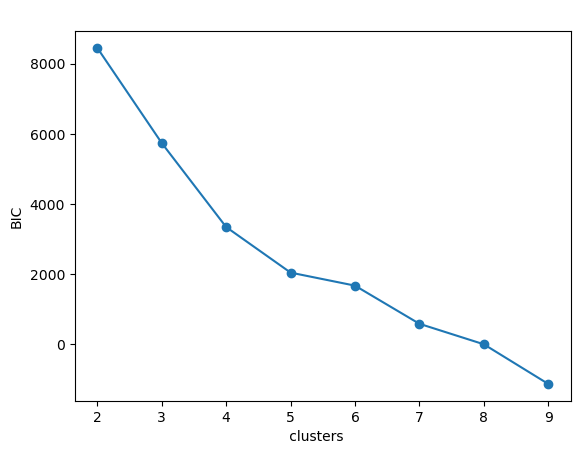
\includegraphics[width=\textwidth]{ch4/assets/BICoriginal.png}
  \centerline{(a) Dados Originais (ao minuto)}
\end{minipage}
\hfill
\begin{minipage}{0.48\textwidth}
  \centering
  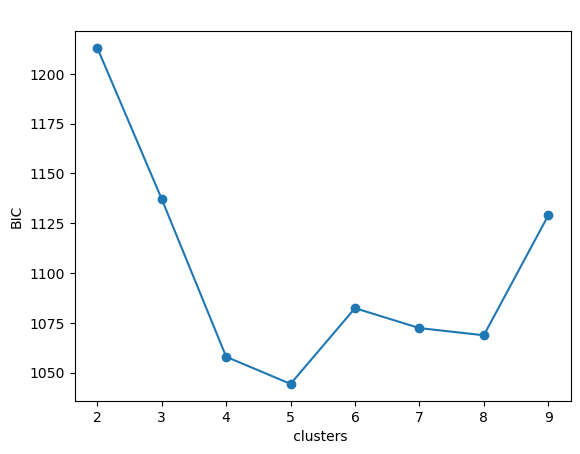
\includegraphics[width=\textwidth]{ch4/assets/BICjanela.png}
  \centerline{(b) Janelas de 10 Minutos}
\end{minipage}
\caption{Curvas do Bayesian Information Criterion (BIC) obtidas para o modelo GMM.}
\label{fig:bic_curves}
\end{figure}

O critério BIC penaliza a complexidade excessiva do modelo, sendo que valores inferiores indicam melhor adequação e separação teórica dos dados. Nas curvas da Figura \ref{fig:bic_curves}, observa-se que, para os dados originais ao minuto (Figura \ref{fig:bic_curves}a), o BIC decresce continuamente sugerindo 9 clusters. Contudo, teorias matemáticas à parte, esta partição gera uma fragmentação excessiva que compromete a utilidade prática dos estados. Este problema foi mitigado na versão com janelas de 10 minutos (Figura \ref{fig:bic_curves}b), onde a suavização do ruído fisiológico revelou um mínimo global côncavo claro em exatamente 5 clusters, definindo o ponto ideal de equilíbrio matemático e interpretabilidade.

\item \textbf{Seleção Estrutural dos Clusters CHA ($k$):} No \textit{Clustering Hierárquico Aglomerativo}, a configuração final de \textit{$k=5$} também foi definida com base na análise conjunta do \textit{Silhouette Score}, da curva do cotovelo (\textit{Elbow Method}) e do dendrograma. Embora algumas métricas automáticas sugerissem um número inferior de clusters, a escolha de cinco agrupamentos representou o melhor compromisso entre qualidade estrutural e interpretabilidade fisiológica dos estados identificados.

A Figura \ref{fig:elbow_curves} exibe as \textbf{curvas do cotovelo} obtidas para o modelo de Clustering Hierárquico treinado, respetivamente, com os dados originais ao nível do minuto e com os dados agregados em janelas de 10 minutos. Estas curvas representam a evolução da soma dos quadrados intra-cluster (WCSS), métrica que avalia a coesão dos grupos. Quanto menor o WCSS, mais próximas se encontram as amostras dentro de cada cluster. Contudo, o objetivo não consiste em obter o menor valor possível de WCSS, uma vez que esta métrica diminui naturalmente à medida que aumenta o número de clusters. Assim, procura-se identificar o ponto a partir do qual a redução do WCSS deixa de ser significativa, conhecido como o ``cotovelo''. Em ambos os casos observa-se uma diminuição acentuada do WCSS à medida que aumenta o número de clusters, seguida de uma estabilização gradual da curva. Nos dados agregados por janelas, os valores de WCSS são inferiores, refletindo a redução da variabilidade dos sinais após a agregação temporal. Embora a curva não apresente um ponto de quebra perfeitamente definido, permitiu identificar uma região de estabilização posteriormente confirmada pela análise do Silhouette Score e do dendrograma.

\end{itemize}

\begin{figure}[H]
\centering
\begin{minipage}{0.48\textwidth}
  \centering
  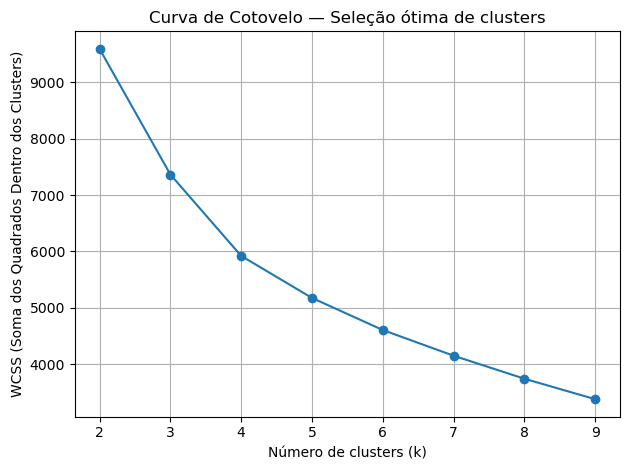
\includegraphics[width=\textwidth]{ch4/assets/cotoveloOriginal.png}
  \centerline{(a) Dados Originais (ao minuto)}
\end{minipage}
\hfill
\begin{minipage}{0.48\textwidth}
  \centering
  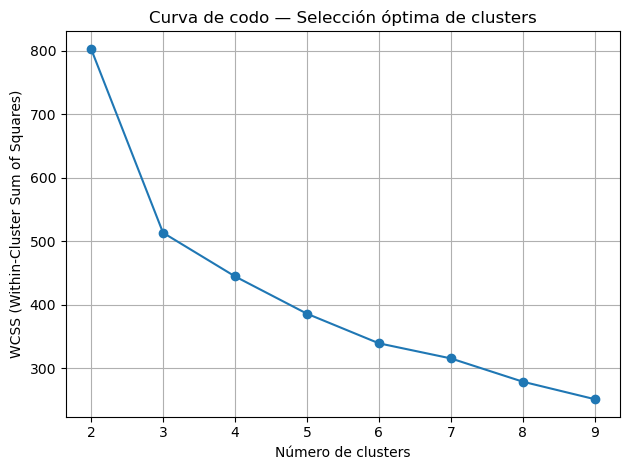
\includegraphics[width=\textwidth]{ch4/assets/cotoveloJanela.png}
  \centerline{(b) Janelas de 10 Minutos}
\end{minipage}
\caption{Curvas do cotovelo (Elbow Method) baseadas no WCSS obtidas para o Clustering Hierárquico.}
\label{fig:elbow_curves}
\end{figure}

As Figuras \ref{fig:silhouette_curves}a e \ref{fig:silhouette_curves}b apresentam a evolução do coeficiente de Silhouette para diferentes números de clusters nos conjuntos de dados originais e agregados por janelas temporais, respetivamente. Esta métrica avalia simultaneamente a coesão interna de cada cluster e a separação entre clusters distintos, assumindo valores entre -1 e 1, sendo que valores mais elevados indicam agrupamentos de melhor qualidade. Nos dados originais, o valor máximo é obtido para $k=8$. No entanto, observa-se que, a partir de aproximadamente cinco clusters, o coeficiente entra numa região relativamente estável, apresentando apenas pequenas variações até ao valor máximo. Isto indica que diferentes soluções nesse intervalo apresentam uma qualidade semelhante do ponto de vista geométrico. Nos dados agregados por janelas, o maior valor ocorre para $k=2$, sugerindo uma divisão muito simples dos dados em dois grandes grupos. Contudo, essa solução revelou-se insuficiente para representar a diversidade dos estados fisiológicos observados ao longo do dia. Para $k=5$, o coeficiente de Silhouette mantém um valor competitivo, permitindo simultaneamente uma descrição mais detalhada dos diferentes estados fisiológicos.

\begin{figure}[H]
\centering
\begin{minipage}{0.48\textwidth}
  \centering
  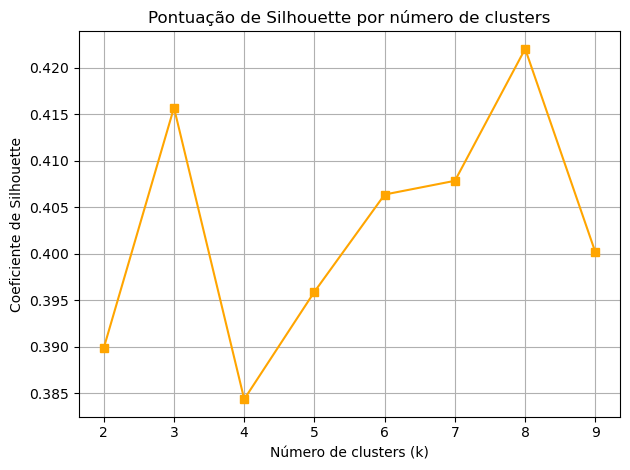
\includegraphics[width=\textwidth]{ch4/assets/silhouetteOriginal.png}
  \centerline{(a) Dados Originais (ao minuto)}
\end{minipage}
\hfill
\begin{minipage}{0.48\textwidth}
  \centering
  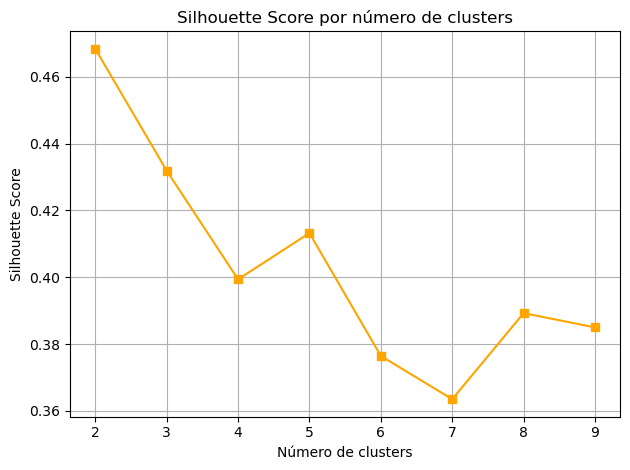
\includegraphics[width=\textwidth]{ch4/assets/silhouetteJanela.png}
  \centerline{(b) Janelas de 10 Minutos}
\end{minipage}
\caption{Evolução do coeficiente de Silhouette para diferentes números de clusters ($k$).}
\label{fig:silhouette_curves}
\end{figure}

As Figuras \ref{fig:dendrogram_original} e \ref{fig:dendrogram_window} apresentam os \textbf{dendrogramas} dos modelos de Clustering Hierárquico treinados, respetivamente, com os dados originais (ao nível do minuto) e com os dados agregados em janelas temporais de 10 minutos. O dendrograma representa o processo de agrupamento hierárquico, mostrando a distância a que os diferentes grupos são sucessivamente unidos: ligações a menores distâncias indicam grupos mais semelhantes, enquanto ligações a maiores distâncias correspondem a grupos mais distintos. Comparando ambos os modelos, observa-se que os dados originais apresentam uniões a distâncias mais elevadas, refletindo a maior variabilidade dos sinais fisiológicos. Já nos dados agregados em janelas temporais, essas uniões ocorrem a distâncias inferiores, originando uma estrutura mais compacta e homogénea, o que indica que a agregação temporal reduziu parte dessa variabilidade e favoreceu a formação de estados fisiológicos mais estáveis.

O dendrograma permite ainda explorar diferentes soluções de agrupamento (diferentes números de clusters, $k$) através da definição de um nível de corte horizontal. O número de ramos intercetados por essa linha corresponde ao número de grupos obtidos: um corte mais elevado produz poucos agrupamentos, mais gerais, enquanto um corte mais baixo origina um maior número de grupos e uma segmentação mais detalhada. No modelo treinado com os dados originais, por exemplo, um corte próximo da distância 100 resulta em dois grandes grupos, correspondendo provavelmente a uma separação entre períodos de sono e de vigília. Reduzindo o nível de corte para aproximadamente 40, obtêm-se cinco clusters, permitindo distinguir diferentes estados fisiológicos sem fragmentar excessivamente os dados. Assim, embora o dendrograma, por si só, não determine o número ótimo de clusters, a sua análise visual complementou a curva do cotovelo e o coeficiente de Silhouette, sustentando a adoção de uma configuração final de cinco clusters por representar o melhor compromisso entre a qualidade do agrupamento e a interpretação fisiológica dos estados identificados.

\begin{figure}[H]
\centering
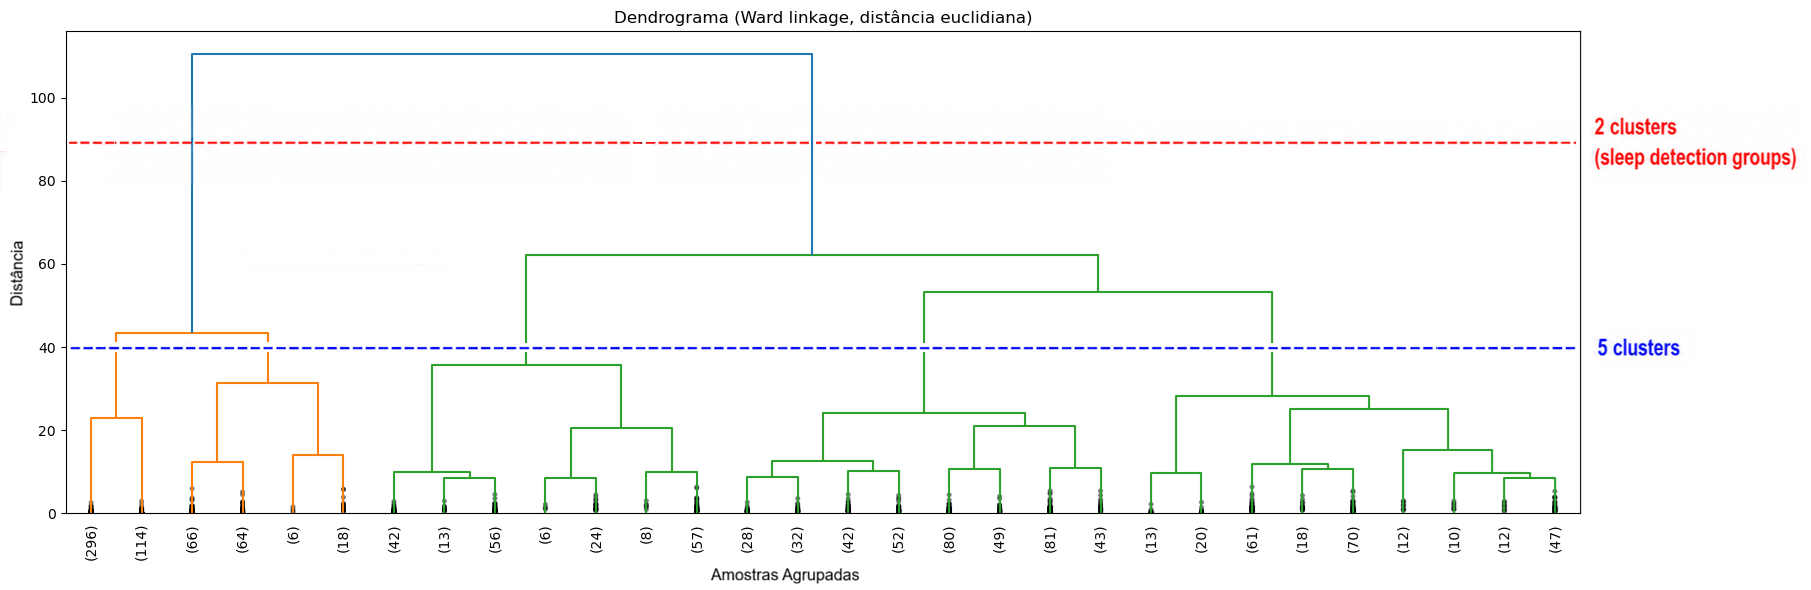
\includegraphics[width=1\textwidth]{ch4/assets/dendrogamaOriginal.png}
\caption{Dendrograma - Dados Originais}
\label{fig:dendrogram_original}
\end{figure}

\begin{figure}[H]
\centering
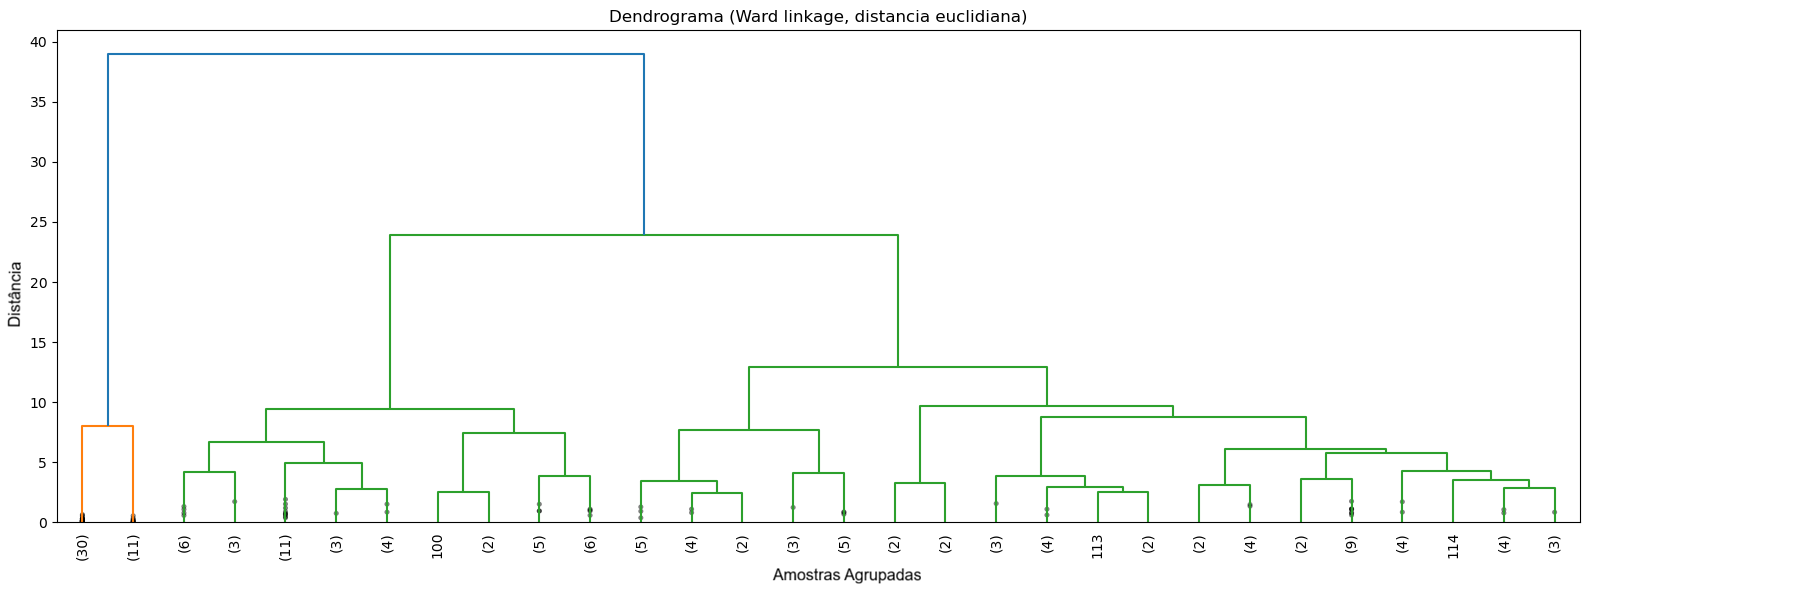
\includegraphics[width=1\textwidth]{ch4/assets/dendrogamaJanela.png}
\caption{Dendrograma - Janelas de 10 minutos}
\label{fig:dendrogram_window}
\end{figure}

Considerando em conjunto o Silhouette Score, a curva do cotovelo, o dendrograma e a necessidade de obter grupos com significado fisiológico, foi adotada uma configuração final de cinco clusters para o modelo hierárquico.

\paragraph{Interpretabilidade dos Clusters Hierárquicos (Árvores de Decisão)}

Para avaliar a consistência dos agrupamentos obtidos nas partições do Clustering Hierárquico Aglomerativo, foi treinada uma Árvore de Decisão utilizando as variáveis fisiológicas como atributos de entrada e os clusters produtos por esse algoritmo como variável-alvo. A Tabela \ref{tab:arvore_validacao} apresenta os resultados obtidos.

\begin{table}[H]
\centering
\caption{Avaliação da Interpretabilidade através de Árvore de Decisão}
\label{tab:arvore_validacao}
\footnotesize
\resizebox{\textwidth}{!}{%
\begin{tabular}{l c c c}
\hline
Configuração & Profundidade Máxima & Accuracy Treino & Accuracy (5-Fold CV) \\
\hline
Dados Originais & 8 & 98.61\% & 92.01\% $\pm$ 4.44\% \\
Janelas (10 min) & 5 & 93.06\% & 83.92\% $\pm$ 10.24\% \\
\hline
\end{tabular}%
}
\end{table}

Os resultados demonstram que os clusters obtidos apresentam fronteiras suficientemente consistentes para serem reproduzidas por um modelo supervisionado simples. Nos dados originais foi obtida uma \textit{accuracy} de validação cruzada de 92.01\%, enquanto a abordagem baseada em janelas temporais alcançou 83.92\%. Embora este último valor seja inferior, continua a evidenciar uma boa capacidade de generalização, tendo em consideração que o número de observações foi reduzido de aproximadamente 1440 para apenas 144 amostras após o processo de agregação temporal, correspondentes às 24 horas de uma jornada laboral completa.

A estrutura de decisão destas árvores, as quais indicam de forma explícita os caminhos e as regras de corte lógicas para a atribuição de cada cluster com base no critério de impureza de Gini, encontra-se representada graficamente nas Figuras \ref{fig:arvore_jerarquico_original} e \ref{fig:arvore_jerarquico_window}. Através delas, é possível observar claramente como as regras lógicas são formadas sequencialmente a partir de variáveis fisiológicas e de movimento. Esta disparidade de complexidade estrutural possivelmente deve-se ao facto de o modelo original operar com dados ao nível do minuto, lidando com flutuações rápidas e maior ruído, o que fez com que a árvore de crescimento livre se expandisse até 8 níveis de profundidade real (ao contrário do modelo de janelas de 10 minutos, que alcançou apenas 5 níveis).

\begin{figure}[H]
\centering
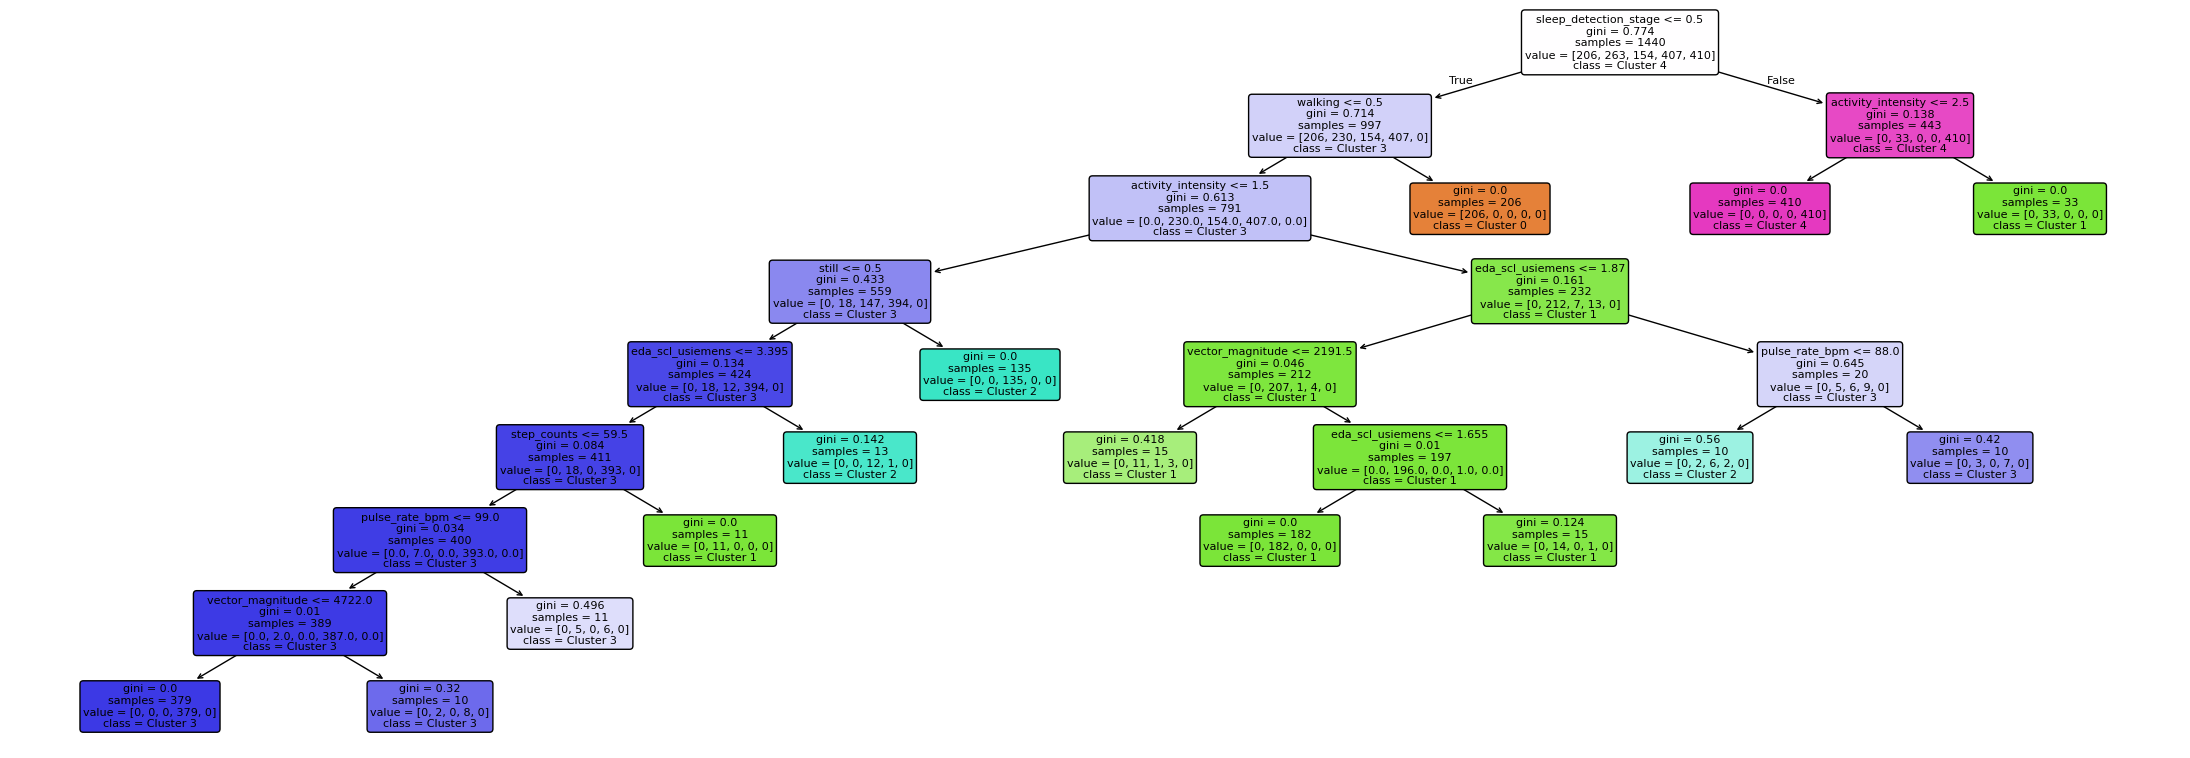
\includegraphics[width=1\textwidth]{ch4/assets/jerarquico1min.png}
\caption{Árvore de Decisão treinada com base no índice de Gini usando os dados ao minuto.}
\label{fig:arvore_jerarquico_original}
\end{figure}

\begin{figure}[H]
\centering
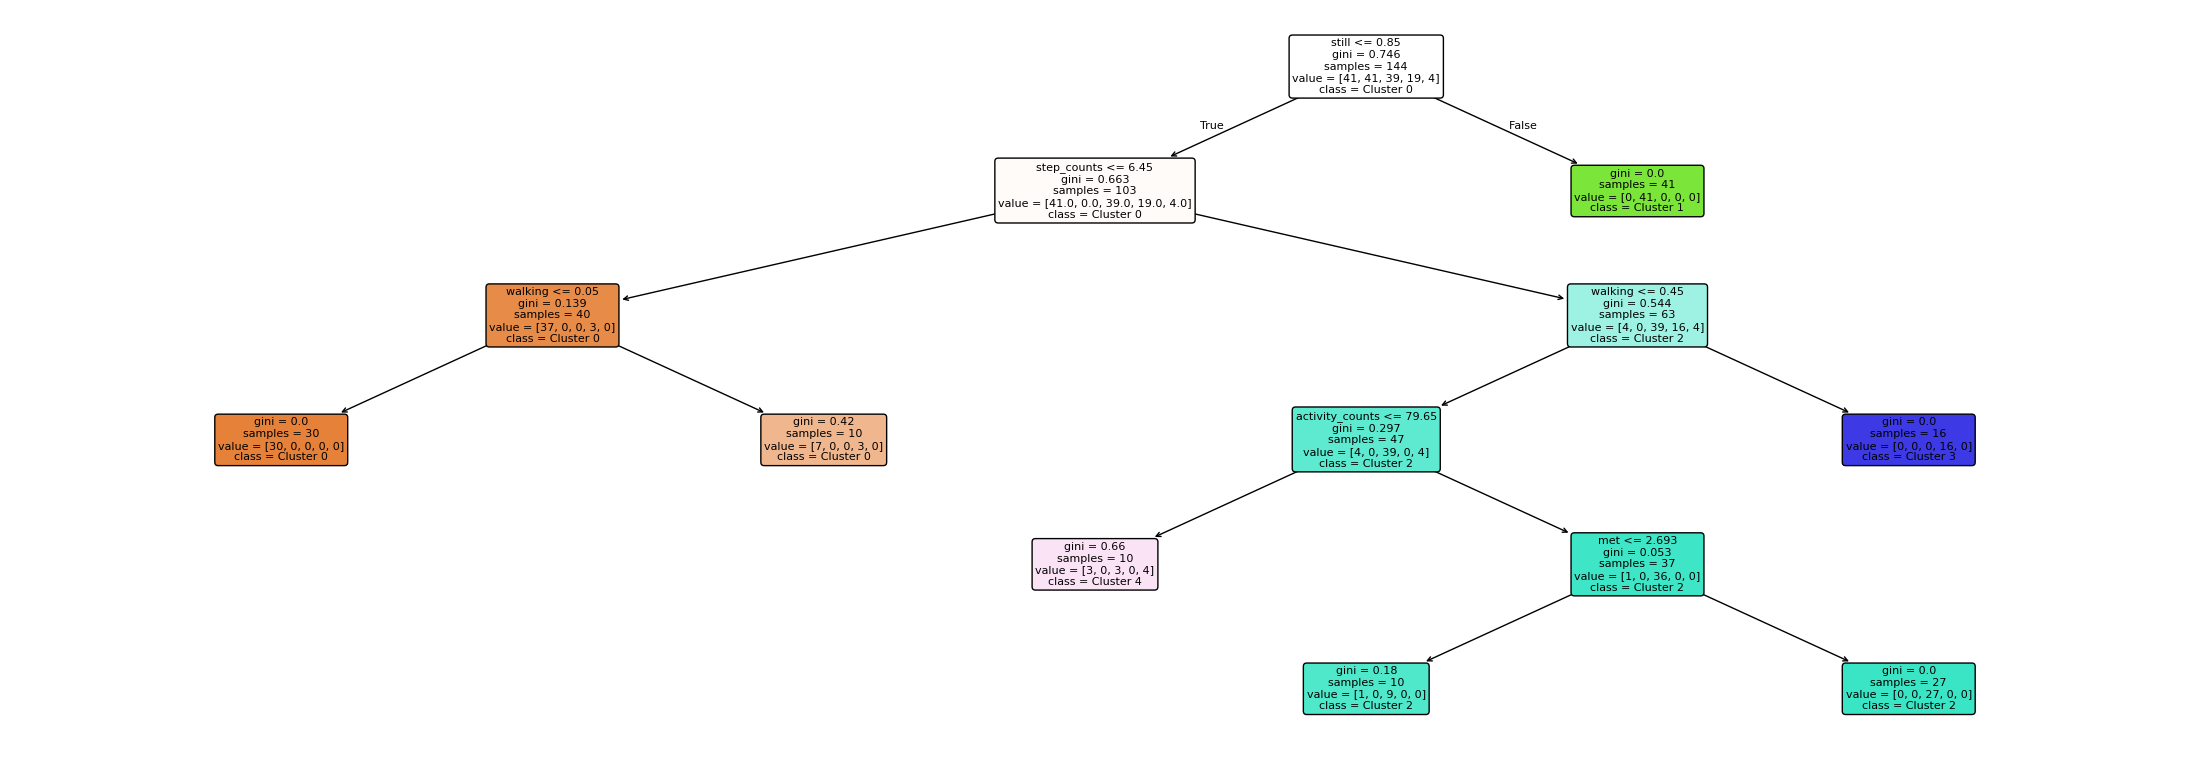
\includegraphics[width=1\textwidth]{ch4/assets/jerarquico10min.png}
\caption{Árvore de Decisão detalhada com critério de Gini usando os dados em janelas de 10 minutos.}
\label{fig:arvore_jerarquico_window}
\end{figure}

\clearpage
As regras de inferência lógica extraídas das árvores de decisão em ambos os cenários são apresentadas em formato textual a seguir. Na Tabela \ref{tab:regras_originais} constam as regras baseadas no conjunto de dados original de resolução de um minuto, onde sobressai a relevância da fase do sono e da intensidade de atividade na separação rápida dos agrupamentos. Por sua vez, a Tabela \ref{tab:regras_janelas} ilustra os caminhos de decisão para o cenário de janelas de 10 minutos, consolidando como a lógica transita para limites baseados em quantidades cumulativas físicas de movimento e repouso de duração contínua.

\begin{table}[H]
\centering
\caption{Regras de Decisão para a Identificação de Clusters (Dados Originais)}
\label{tab:regras_originais}
\resizebox{\textwidth}{!}{%
\begin{tabular}{l}
\hline
\textbf{Regras Lógicas Extraídas (Resolução Temporal: 1 minuto)} \\
\hline
Se \textbf{\texttt{sleep\_detection\_stage}} $\le 0.50$: \\
~~Se \textbf{\texttt{walking}} $\le 0.50$: \\
~~~~Se \textbf{\texttt{activity\_intensity}} $\le 1.50$: \\
~~~~~~Se \textbf{\texttt{still}} $\le 0.50$: \\
~~~~~~~~Se \textbf{\texttt{eda\_scl\_usiemens}} $\le 3.39$: \\
~~~~~~~~~~Se \textbf{\texttt{step\_counts}} $\le 59.50$: \\
~~~~~~~~~~~~Se \textbf{\texttt{pulse\_rate\_bpm}} $\le 99.00$: \\
~~~~~~~~~~~~~~Se \textbf{\texttt{vector\_magnitude}} $\le 4722.00 \rightarrow$ \textbf{Cluster 3} (Atividade de transição/baixo movimento) \\
~~~~~~~~~~~~~~Se \textbf{\texttt{vector\_magnitude}} $> 4722.00 \rightarrow$ \textbf{Cluster 3} (Atividade residual física em repouso) \\
~~~~~~~~~~~~~~Se \textbf{\texttt{pulse\_rate\_bpm}} $> 99.00 \rightarrow$ \textbf{Cluster 3} (Ativação fisiológica pontual sem locomoção) \\
~~~~~~~~~~Se \textbf{\texttt{step\_counts}} $> 59.50 \rightarrow$ \textbf{Cluster 1} (Fração de movimento transicional ligeiro) \\
~~~~~~~~Se \textbf{\texttt{eda\_scl\_usiemens}} $> 3.39 \rightarrow$ \textbf{Cluster 2} (Trabalho estático com elevada reatividade simpática) \\
~~~~~~Se \textbf{\texttt{still}} $> 0.50 \rightarrow$ \textbf{Cluster 2} (Trabalho sedentário/estático padrão) \\
~~~~Se \textbf{\texttt{activity\_intensity}} $> 1.50$: \\
~~~~~~Se \textbf{\texttt{eda\_scl\_usiemens}} $\le 1.87 \rightarrow$ \textbf{Cluster 1} (Esforço físico leve com baixa condutância eletrodérmica) \\
~~~~~~Se \textbf{\texttt{eda\_scl\_usiemens}} $> 1.87 \rightarrow$ \textbf{Cluster 3} (Esforço físico moderado com maior ativação simpática) \\
~~Se \textbf{\texttt{walking}} $> 0.50 \rightarrow$ \textbf{Cluster 0} (Atividade física de caminhada) \\
Se \textbf{\texttt{sleep\_detection\_stage}} $> 0.50$: \\
~~Se \textbf{\texttt{activity\_intensity}} $\le 2.50 \rightarrow$ \textbf{Cluster 4} (Fase de repouso ou sono profundo com baixa ativação) \\
~~Se \textbf{\texttt{activity\_intensity}} $> 2.50 \rightarrow$ \textbf{Cluster 1} (Fase de repouso com transições de movimento leve) \\
\hline
\end{tabular}%
}
\end{table}

\begin{table}[H]
\centering
\caption{Regras de Decisão para a Identificação de Clusters (Janelas de 10 min)}
\label{tab:regras_janelas}
\resizebox{\textwidth}{!}{%
\begin{tabular}{l}
\hline
\textbf{Regras Lógicas Extraídas (Agregação Temporal: Janelas de 10 minutos)} \\
\hline
Se \textbf{\texttt{still}} $\le 0.85$: \\
~~Se \textbf{\texttt{step\_counts}} $\le 6.45$: \\
~~~~Se \textbf{\texttt{walking}} $\le 0.05$ $\rightarrow$ \textbf{Cluster 0} (Transições breves de movimento sedentário) \\
~~~~Se \textbf{\texttt{walking}} $> 0.05$ $\rightarrow$ \textbf{Cluster 0} (Transições de caminhada muito leve pontual) \\
~~Se \textbf{\texttt{step\_counts}} $> 6.45$: \\
~~~~Se \textbf{\texttt{walking}} $\le 0.45$: \\
~~~~~~Se \textbf{\texttt{activity\_counts}} $\le 79.65$ $\rightarrow$ \textbf{Cluster 4} (Trabalho com movimentação generalizada em ritmo calmo) \\
~~~~~~Se \textbf{\texttt{activity\_counts}} $> 79.65$: \\
~~~~~~~~Se \textbf{\texttt{met}} $\le 2.69$ $\rightarrow$ \textbf{Cluster 2} (Trabalho físico leve com carga metabólica controlada) \\
~~~~~~~~Se \textbf{\texttt{met}} $> 2.69$ $\rightarrow$ \textbf{Cluster 2} (Atividade laboral ativa integrada de movimento variado) \\
~~~~Se \textbf{\texttt{walking}} $> 0.45$ $\rightarrow$ \textbf{Cluster 3} (Atividade contínua ou prolongada de caminhada ativa) \\
Se \textbf{\texttt{still}} $> 0.85$ $\rightarrow$ \textbf{Cluster 1} (Estado estático dominante - repouso consolidado ou sono estável) \\
\hline
\end{tabular}%
}
\end{table}

A Tabela \ref{tab:importancia_gini} apresenta a importância relativa das principais variáveis fisiológicas, calculada através do índice de impureza de Gini (\textit{Gini Importance} ou \textit{Mean Decrease in Impurity}), utilizadas pela Árvore de Decisão para distinguir os diferentes clusters. Os resultados dividem-se entre os dados originais e após a agregação temporal de 10 minutos, ordenados de forma decrescente de importância.

\begin{table}[H]
\centering
\caption{Importância Relativa das Variáveis na Árvore de Decisão (Ordenada)}
\label{tab:importancia_gini}
\resizebox{\textwidth}{!}{%
\begin{tabular}{l c p{0.5cm} l c}
\hline
\multicolumn{2}{c}{\textbf{Dados Originais}} & & \multicolumn{2}{c}{\textbf{Janelas Temporais (10 min)}} \\
\cline{1-2} \cline{4-5}
Variável & Importância & & Variável & Importância \\
\hline
\texttt{sleep\_detection\_stage} & 31.47\% & & \texttt{still} & 41.34\% \\
\texttt{activity\_intensity} & 24.54\% & & \texttt{step\_counts} & 29.95\% \\
\texttt{walking} & 20.88\% & & \texttt{walking} & 22.85\% \\
\texttt{still} & 17.06\% & & \texttt{activity\_counts} & 5.70\% \\
\texttt{eda\_scl\_usiemens} & 3.25\% & & \texttt{met} & 0.15\% \\
\texttt{step\_counts} & 1.90\% & & \texttt{pulse\_rate\_bpm} & 0.00\% \\
\texttt{pulse\_rate\_bpm} & 0.68\% & & \texttt{eda\_scl\_usiemens} & 0.00\% \\
\texttt{vector\_magnitude} & 0.21\% & & \texttt{activity\_intensity} & 0.00\% \\
\texttt{met} & 0.00\% & & \texttt{vector\_magnitude} & 0.00\% \\
\texttt{activity\_counts} & 0.00\% & & \texttt{sleep\_detection\_stage} & 0.00\% \\
\texttt{generic} & 0.00\% & & \texttt{generic} & 0.00\% \\
\hline
\end{tabular}%
}
\end{table}

A análise da importância das variáveis na Árvore de Decisão mostra que a explicação dos clusters permanece globalmente consistente entre as duas representações dos dados. Em ambos os casos, variáveis relacionadas com a atividade e o movimento, como \texttt{walking} e \texttt{still}, mantêm elevada relevância. Nos dados originais, a variável \texttt{sleep\_detection\_stage} assume a maior importância (31.47\%), enquanto na abordagem baseada em janelas temporais a sua contribuição deixa de ser significativa, sendo substituída por indicadores mais agregados da atividade, como \texttt{step\_counts}. De forma semelhante, a variável \texttt{activity\_intensity} perde relevância, sendo substituída por métricas relacionadas com a quantidade de movimento, que representam informação semelhante sobre o nível de atividade do utilizador.

Esta alteração é consistente com o efeito da agregação temporal. Nos dados ao nível do minuto, a variável \texttt{sleep\_detection\_stage} identifica diretamente o estado de sono e, por isso, constitui o principal fator de decisão da árvore. No entanto, ao agregar os dados em janelas de 10 minutos, o comportamento do utilizador passa a ser descrito por indicadores mais estáveis, como a permanência em repouso (\texttt{still}) e o número de passos (\texttt{step\_counts}), tornando a informação explícita sobre o estágio do sono menos determinante para distinguir os diferentes clusters. Estes resultados sugerem que a agregação temporal não altera significativamente os padrões fisiológicos identificados, mas modifica as variáveis mais relevantes para a sua interpretação, privilégindo medidas representativas do comportamento observado ao longo do janela temporal.

\paragraph{Classificação e Interpretação Fisiológica dos Clusters}

Um passo fundamental desta investigação consistiu na interpretação dos clusters gerados pelos diferentes modelos de agrupamento. Para além de identificar o número ótimo de grupos, foi necessário compreender o significado das divisões produzidas pelos algoritmos, analisando porque determinados registos fisiológicos eram agrupados entre si e que estados físicos ou comportamentais poderiam estar a ser representados. O objetivo não foi apenas avaliar o desempenho matemático dos modelos, mas também verificar se os clusters correspondiam a estados fisiológicos reais e interpretáveis, capazes de descrever diferentes momentos da rotina diária do indivíduo.

Para esse efeito, a interpretação dos clusters baseou-se em duas fontes de informação complementares:
\begin{itemize}
    \item \textbf{A distribuição por percentis relativos (\textit{LOW, MED, HIGH})} de cada variável fisiológica e comportamental dentro do cluster, permitindo compreender a assinatura neurofisiológica biológica do estado.
    \item \textbf{A distribuição temporal diária dos clusters}, analisando a sua ocorrência ao longo das 24 horas e verificando se os estados identificados surgiam em períodos coerentes com atividades como o sono, o trabalho, os deslocamentos ou os momentos de maior esforço físico.
\end{itemize}

\setlength{\leftmargini}{0pt}
\begin{enumerate}
    \item \textbf{Modelo GMM Original ($k=9$):}
    
    Para o modelo probabilístico inicial de referência, o \textbf{Gaussian Mixture Model (GMM) com dados originais ($k=9$)}, este estudo permitiu cartografar com elevado detalhe a assinatura de cada agrupamento, conforme apresentado na Tabela \ref{tab:percentis_gmm_original}.

    \begin{table}[H]
    \centering
    \caption{Assinatura Fisiológica e Sensibilidade dos Clusters para o GMM de Dados Originais ($k=9$, Dados ao Minuto)}
    \label{tab:percentis_gmm_original}
    \renewcommand{\arraystretch}{1.4}
    \resizebox{\textwidth}{!}{%
    \begin{tabular}{c c c c c c c c c c}
    \hline
    \textbf{Cluster} & \textbf{EDA} & \textbf{Pulse Rate} & \textbf{MET} & \textbf{Act. Counts} & \textbf{Step Counts} & \textbf{Vec. Mag.} & \textbf{Act. Intensity} & \textbf{Sleep Stage} & \textbf{Significado Fisiológico Proposto} \\
    \hline
    5 & \textit{LOW} & \textit{MED} & \textit{LOW} & \textit{LOW} & \textit{LOW} & \textit{LOW} & \textit{LOW} & \textit{HIGH} & [Grupo de sono] início \\
    0 & \textit{MED} & \textit{LOW} & \textit{LOW} & \textit{LOW} & \textit{LOW} & \textit{LOW} & \textit{LOW} & \textit{HIGH} & [Grupo de sono] profundo \\
    1 & \textit{LOW} & \textit{MED} & \textit{HIGH} & \textit{MED} & \textit{HIGH} & \textit{HIGH} & \textit{HIGH} & \textit{HIGH} & [Grupo de despertar] \\
    7 & \textit{HIGH} & \textit{MED} & \textit{MED} & \textit{LOW} & \textit{MED} & \textit{MED} & \textit{MED} & \textit{HIGH} & [Grupo de sedentarismo/foco] estado base \\
    2 & \textit{HIGH} & \textit{MED} & \textit{MED} & \textit{MED} & \textit{MED} & \textit{MED} & \textit{MED} & \textit{LOW} & [Grupo de sedentarismo/foco] trabalho/concentração \\
    6 & \textit{HIGH} & \textit{LOW} & \textit{MED} & \textit{MED} & \textit{MED} & \textit{MED} & \textit{MED} & \textit{LOW} & [Grupo de sedentarismo/foco] pico stress \\
    3 & \textit{LOW} & \textit{HIGH} & \textit{HIGH} & \textit{HIGH} & \textit{HIGH} & \textit{HIGH} & \textit{HIGH} & \textit{LOW} & [Grupo de atividade física] caminhada \\
    8 & \textit{LOW} & \textit{MED} & \textit{HIGH} & \textit{HIGH} & \textit{HIGH} & \textit{HIGH} & \textit{HIGH} & \textit{LOW} & [Grupo de atividade física] movimento geral \\
    4 & \textit{HIGH} & \textit{HIGH} & \textit{HIGH} & \textit{HIGH} & \textit{HIGH} & \textit{HIGH} & \textit{HIGH} & \textit{LOW} & [Grupo de atividade física] atividade intensa \\
    \hline
    \end{tabular}%
    }
    \end{table}

    A Figura \ref{fig:temporal_gmm_original} ilustra a distribuição temporal dos clusters identificados pelo GMM com dados originais ao minuto ($k=9$) ao longo de uma jornada laboral completa (00:00--23:59), permitindo observar como os diferentes estados fisiológicos se sucedem de forma coerente com o ritmo diário do trabalhador.

    \begin{figure}[H]
    \centering
    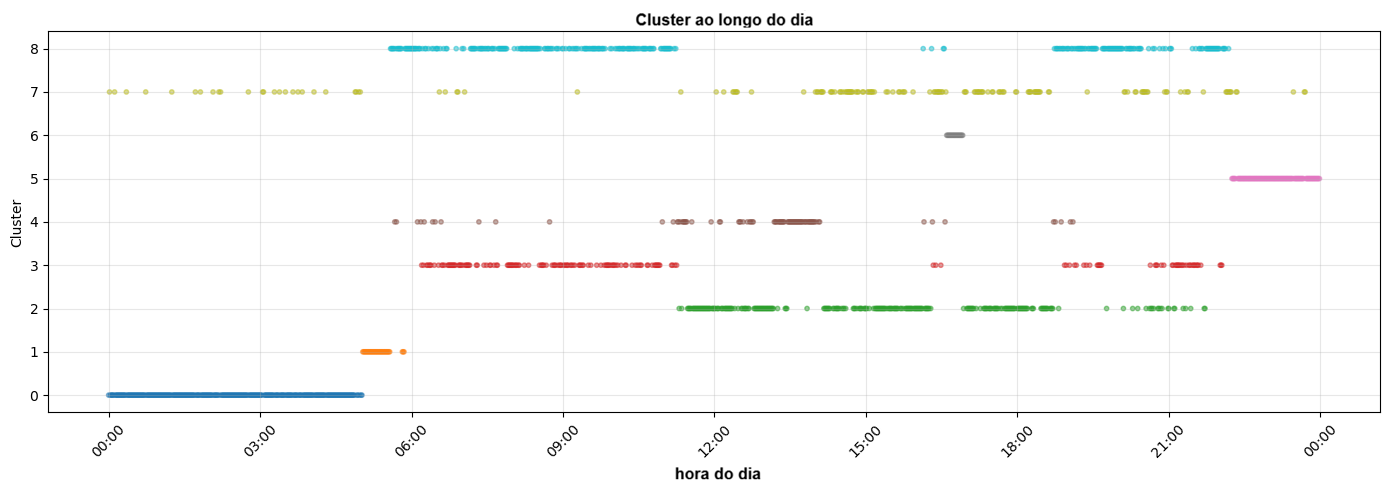
\includegraphics[width=1\textwidth]{ch4/assets/temporalgmmoriginal.png}
    \caption{Distribuição temporal diária dos clusters do GMM (dados ao minuto) ao longo de uma jornada.}
    \label{fig:temporal_gmm_original}
    \end{figure}

    A análise da Tabela \ref{tab:percentis_gmm_original} evidencia que, embora o critério BIC tenha indicado nove clusters como a solução estatisticamente ótima para o GMM, essa segmentação revelou-se demasiado detalhada para uma interpretação fisiológica direta. Observa-se que vários clusters apresentam assinaturas muito semelhantes, diferindo apenas em pequenas variações de algumas variáveis fisiológicas. Assim, em vez de representar nove estados fisiológicos completamente distintos, o modelo descreve diferentes variações de um conjunto mais reduzido de comportamentos.

    Com base nas assinaturas fisiológicas e na distribuição temporal apresentada na Figura \ref{fig:temporal_gmm_original}, foi possível organizar estes nove clusters em quatro grandes grupos funcionais: repouso, despertar, sedentarismo/concentração e atividade física. Dentro de cada grupo, os diferentes clusters representam variações do mesmo estado fisiológico, distinguindo-se sobretudo pela intensidade da atividade, pelo nível de stress ou pela fase do ciclo diário. Esta interpretação permitiu transformar uma solução matematicamente ótima, mas complexa, numa representação mais simples e coerente do comportamento fisiológico observado ao longo do dia.

% ---------------------------------------------------------------
% GMM RESTRITO (k=4) — Dados Originais ao Minuto
% ---------------------------------------------------------------

    \item \textbf{Modelo GMM Restrito ($k=4$):}

    De forma complementar, o \textbf{GMM Restrito ($k=4$)} com dados originais ao minuto foi analisado de forma análoga, conforme apresentado na Tabela \ref{tab:percentis_gmm_restrito}.

    \begin{table}[H]
    \centering
    \caption{Assinatura Fisiológica dos Clusters para o GMM Restrito ($k=4$, Dados ao Minuto)}
    \label{tab:percentis_gmm_restrito}
    \renewcommand{\arraystretch}{1.4}
    \resizebox{\textwidth}{!}{%
    \begin{tabular}{c c c c c c c c c c}
    \hline
    \textbf{Cluster} & \textbf{EDA} & \textbf{Pulse Rate} & \textbf{MET} & \textbf{Act. Counts} & \textbf{Step Counts} & \textbf{Vec. Mag.} & \textbf{Act. Intensity} & \textbf{Sleep Stage} & \textbf{Significado Fisiológico Proposto} \\
    \hline
    0 & \textit{MED} & \textit{LOW} & \textit{LOW} & \textit{LOW} & \textit{LOW} & \textit{LOW} & \textit{LOW} & \textit{HIGH} & Repouso e Sono Profundo \\
    1 & \textit{HIGH} & \textit{MED} & \textit{HIGH} & \textit{HIGH} & \textit{HIGH} & \textit{HIGH} & \textit{HIGH} & \textit{LOW} & Trabalho Ativo / Jornada Operativa \\
    2 & \textit{HIGH} & \textit{MED} & \textit{MED} & \textit{MED} & \textit{HIGH} & \textit{MED} & \textit{MED} & \textit{HIGH} & Sedentarismo em Alerta / Transições \\
    3 & \textit{MED} & \textit{HIGH} & \textit{HIGH} & \textit{HIGH} & \textit{HIGH} & \textit{HIGH} & \textit{HIGH} & \textit{LOW} & Atividade Física e Deslocamentos \\
    \hline
    \end{tabular}%
    }
    \end{table}

    A Figura \ref{fig:temporal_gmm_restrito} ilustra a distribuição temporal dos clusters do GMM Restrito ($k=4$) ao longo de uma jornada completa.

    \begin{figure}[H]
    \centering
    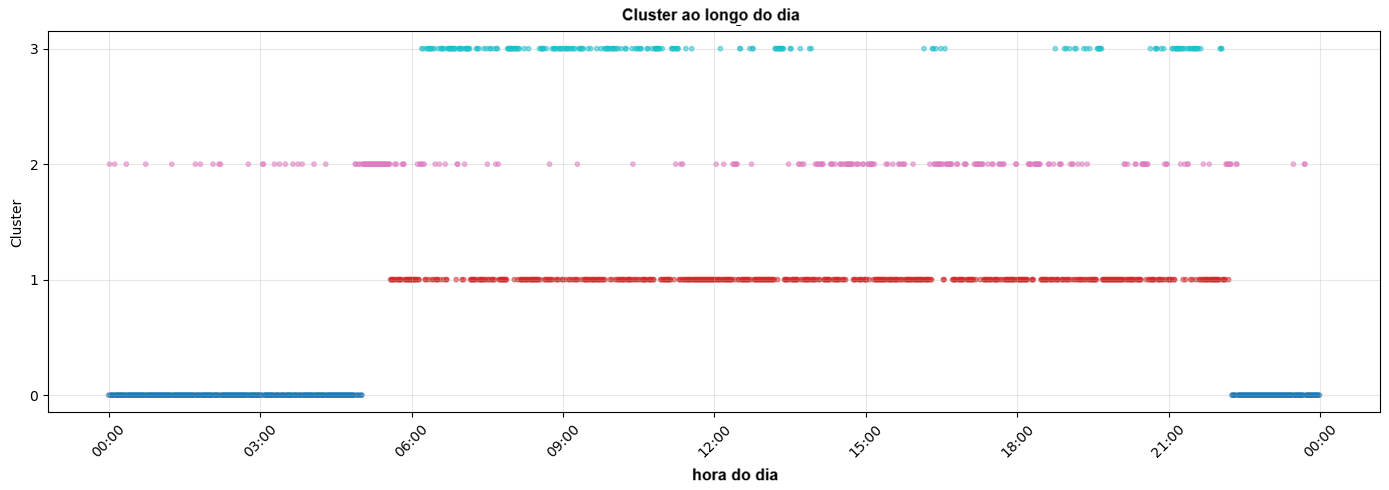
\includegraphics[width=1\textwidth]{ch4/assets/temporalgmmrestricto.png}
    \caption{Distribuição temporal diária dos clusters do GMM Restrito ($k=4$, dados ao minuto) ao longo de uma jornada.}
    \label{fig:temporal_gmm_restrito}
    \end{figure}

    O GMM Restrito ($k=4$) foi desenvolvido com o objetivo de reduzir a fragmentação observada na solução original de nove clusters, fundindo automaticamente os clusters mais semelhantes numa representação mais simples e interpretável. A interpretação fisiológica resultou da combinação da assinatura das variáveis (Tabela \ref{tab:percentis_gmm_restrito}) com a sua distribuição temporal (Figura \ref{fig:temporal_gmm_restrito}). O cluster Repouso e Sono Profundo concentra-se durante a noite e caracteriza-se por baixa atividade e elevados valores de Sleep Stage. O cluster Atividade Física e Deslocamentos apresenta valores elevados de frequência cardíaca, MET e passos, surgindo de forma intermitente ao longo do dia. O cluster Trabalho Ativo / Jornada Operativa predomina entre as 06:00 e as 22:00, combinando elevada atividade, passos e EDA, compatíveis com uma atividade laboral ativa. Por fim, o cluster Sedentarismo em Alerta / Transições apresenta atividade moderada, EDA elevada e valores elevados de Sleep Stage, sugerindo situações de reduzido movimento associadas a atividade cognitiva durante o dia ou a episódios de sono leve durante a noite.

    De um modo geral, o GMM Restrito conseguiu reduzir a fragmentação observada na solução com nove clusters, fundindo automaticamente estados fisiológicos muito semelhantes e produzindo uma representação mais simples. A distinção entre os períodos de sono e vigília manteve-se clara, evidenciando que essa separação corresponde ao padrão fisiológico dominante dos dados. No entanto, os restantes clusters apresentam uma distribuição temporal bastante sobreposta, coexistindo frequentemente nos mesmos períodos do dia e alternando de forma muito rápida. Este comportamento sugere que a fusão dos clusters simplificou excessivamente a representação dos estados fisiológicos, reduzindo a capacidade do modelo para distinguir diferentes padrões de atividade ao longo da jornada.
% ---------------------------------------------------------------
% GMM — Janelas de 10 Minutos (k=5)
% ---------------------------------------------------------------

    \item \textbf{Modelo GMM em Janelas de 10 Minutos ($k=5$):}

    Para os dados agregados em janelas de 10 minutos, o \textbf{GMM ($k=5$)} produziu os agrupamentos caracterizados na Tabela \ref{tab:percentis_gmm_janela}.

    \begin{table}[H]
    \centering
    \caption{Assinatura Fisiológica dos Clusters para o GMM ($k=5$, Janelas de 10 min)}
    \label{tab:percentis_gmm_janela}
    \renewcommand{\arraystretch}{1.4}
    \resizebox{\textwidth}{!}{%
    \begin{tabular}{c c c c c c c c c c}
    \hline
    \textbf{Cluster} & \textbf{EDA} & \textbf{Pulse Rate} & \textbf{MET} & \textbf{Act. Counts} & \textbf{Step Counts} & \textbf{Vec. Mag.} & \textbf{Act. Intensity} & \textbf{Sleep Stage} & \textbf{Significado Fisiológico Proposto} \\
    \hline
    0 & \textit{LOW} & \textit{LOW} & \textit{HIGH} & \textit{MED} & \textit{HIGH} & \textit{MED} & \textit{HIGH} & \textit{HIGH} & ``Salto'' da Cama / Transição Matinal \\
    1 & \textit{MED} & \textit{LOW} & \textit{LOW} & \textit{LOW} & \textit{LOW} & \textit{LOW} & \textit{LOW} & \textit{HIGH} & Sono Estável / Estado de Repouso \\
    2 & \textit{HIGH} & \textit{HIGH} & \textit{HIGH} & \textit{HIGH} & \textit{HIGH} & \textit{HIGH} & \textit{HIGH} & \textit{LOW} & Picos de Intensidade Física \\
    3 & \textit{HIGH} & \textit{MED} & \textit{MED} & \textit{MED} & \textit{MED} & \textit{MED} & \textit{MED} & \textit{HIGH} & Jornada Laboral / Carga Cognitiva \\
    4 & \textit{LOW} & \textit{MED} & \textit{HIGH} & \textit{HIGH} & \textit{HIGH} & \textit{HIGH} & \textit{HIGH} & \textit{HIGH} & Rotina Ativa e Deslocamentos \\
    \hline
    \end{tabular}%
    }
    \end{table}

    A Figura \ref{fig:temporal_gmm_janela} ilustra a distribuição temporal dos clusters do GMM com janelas de 10 minutos ao longo de uma jornada completa.

    \begin{figure}[H]
    \centering
    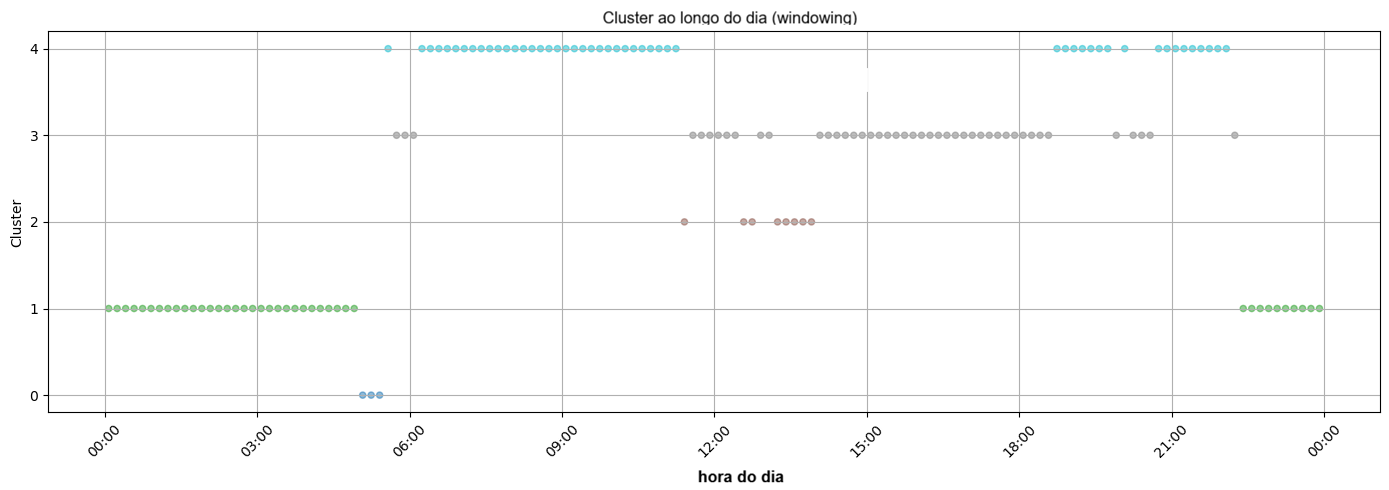
\includegraphics[width=1\textwidth]{ch4/assets/temporalgmmjanela.png}
    \caption{Distribuição temporal diária dos clusters do GMM ($k=5$, janelas de 10 min) ao longo de uma jornada.}
    \label{fig:temporal_gmm_janela}
    \end{figure}

    O GMM treinado com dados agregados em janelas de 10 minutos identificou cinco estados fisiológicos consistentes, interpretados a partir da assinatura das variáveis (Tabela \ref{tab:percentis_gmm_janela}) e da sua distribuição temporal (Figura \ref{fig:temporal_gmm_janela}). O cluster \textit{Sono Estável} concentra-se no período noturno, apresentando baixa atividade física, frequência cardíaca e gasto energético, juntamente com valores elevados de \textit{Sleep Stage}, caracterizando o estado de repouso. Antes do despertar surge um breve cluster de \textit{Transição Matinal}, com MET e passos elevados, mas frequência cardíaca e EDA ainda reduzidas, sugerindo o início do movimento antes da ativação fisiológica completa. Durante a manhã e o início da noite predomina o cluster \textit{Rotina Ativa e Deslocamentos}, marcado por elevados indicadores de movimento e EDA reduzida, compatível com deslocações ou atividade física ligeira. No período central da jornada laboral observa-se o cluster \textit{Jornada Laboral / Carga Cognitiva}, caracterizado por EDA elevada e atividade moderada, refletindo maior exigência mental. Por fim, o cluster \textit{Picos de Intensidade} ocorre apenas pontualmente, apresentando valores elevados na maioria dos indicadores fisiológicos e de movimento, correspondendo aos momentos de maior exigência física.

Visualmente, este modelo apresenta uma evolução temporal mais organizada do que a obtida com os dados ao minuto. Os \textit{clusters} surgem em blocos temporais mais bem definidos, reduzindo as mudanças rápidas entre estados observadas anteriormente. Esta melhoria resulta, provavelmente, da agregação dos dados em janelas de 10 minutos, que reduz as variações instantâneas e o efeito do ruído nas medições. Como consequência, os estados fisiológicos acompanham de forma mais clara a rotina diária do utilizador, passando do repouso para atividades ligeiras, depois para períodos de maior carga cognitiva e, apenas ocasionalmente, para momentos de elevada intensidade física. Esta distribuição está de acordo com o esperado numa jornada diária e mostra que a agregação temporal facilita a identificação de padrões fisiológicos mais estáveis e fáceis de interpretar.    
% ---------------------------------------------------------------
% CLUSTERING HIERÁRQUICO — Dados Originais ao Minuto (k=5)
% ---------------------------------------------------------------

    \item \textbf{Modelo de Clustering Hierárquico Original ($k=5$):}

    No que diz respeito ao \textbf{Clustering Hierárquico Aglomerativo com dados originais ao minuto ($k=5$)}, a caracterização fisiológica dos agrupamentos obtidos é apresentada na Tabela \ref{tab:percentis_hier_original}.

\begin{table}[H]
\centering
\caption{Assinatura Fisiológica dos Clusters para o Clustering Hierárquico ($k=5$, Dados ao Minuto)}
\label{tab:percentis_hier_original}
\renewcommand{\arraystretch}{1.4}
\resizebox{\textwidth}{!}{%
\begin{tabular}{c c c c c c c c c c}
\hline
\textbf{Cluster} & \textbf{EDA} & \textbf{Pulse Rate} & \textbf{MET} & \textbf{Act. Counts} & \textbf{Step Counts} & \textbf{Vec. Mag.} & \textbf{Act. Intensity} & \textbf{Sleep Stage} & \textbf{Significado Fisiológico Proposto} \\
\hline
0 & \textit{MED} & \textit{HIGH} & \textit{HIGH} & \textit{HIGH} & \textit{HIGH} & \textit{HIGH} & \textit{HIGH} & \textit{LOW} & Movimento Ativo e Caminhadas \\
1 & \textit{MED} & \textit{MED} & \textit{HIGH} & \textit{HIGH} & \textit{HIGH} & \textit{HIGH} & \textit{HIGH} & \textit{HIGH} & Atividade com Presença de Sono \\
2 & \textit{HIGH} & \textit{MED} & \textit{MED} & \textit{MED} & \textit{MED} & \textit{MED} & \textit{MED} & \textit{LOW} & Concentração / Carga Cognitiva \\
3 & \textit{HIGH} & \textit{MED} & \textit{MED} & \textit{HIGH} & \textit{HIGH} & \textit{MED} & \textit{MED} & \textit{LOW} & Esforço Físico / Atividade Intensa \\
4 & \textit{MED} & \textit{LOW} & \textit{MED} & \textit{LOW} & \textit{MED} & \textit{LOW} & \textit{MED} & \textit{HIGH} & Repouso ou Sono \\
\hline
\end{tabular}%
}
\end{table}

A Figura \ref{fig:temporal_hier_original} ilustra a distribuição temporal dos clusters do Clustering Hierárquico com dados ao minuto ao longo de uma jornada completa.

\begin{figure}[H]
\centering
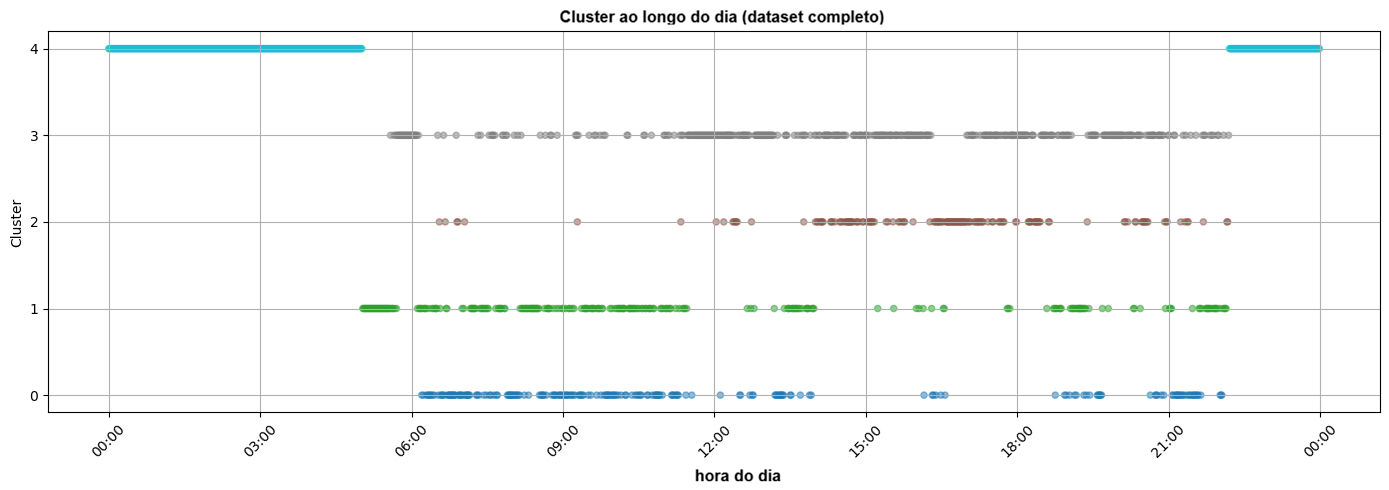
\includegraphics[width=1\textwidth]{ch4/assets/temporalherarquicooriginal.png}
\caption{Distribuição temporal diária dos clusters do Clustering Hierárquico ($k=5$, dados ao minuto) ao longo de uma jornada.}
\label{fig:temporal_hier_original}
\end{figure}

A Figura \ref{fig:temporal_hier_original} apresenta a distribuição temporal dos \textit{clusters} obtidos pelo Clustering Hierárquico com dados ao minuto. Em comparação com o GMM, observa-se uma maior alternância entre estados ao longo do dia, originando transições mais frequentes e uma evolução temporal menos contínua. Apesar de os clusters de \textit{Repouso ou Sono} (Cluster 4) e \textit{Concentração / Carga Cognitiva} (Cluster 2) apresentarem uma distribuição compatível com os períodos noturnos e laborais, respetivamente, os restantes grupos mostram maior dispersão temporal. Em particular, o cluster \textit{Atividade com Presença de Sono} (Cluster 1) apresenta uma assinatura fisiológica pouco intuitiva, combinando elevados níveis de atividade física com valores elevados de \textit{Sleep Stage}, o que dificulta a sua interpretação fisiológica. De forma geral, embora o modelo consiga distinguir estados de repouso, atividade e maior carga cognitiva, a elevada variabilidade temporal e a sobreposição entre alguns clusters tornam a segmentação menos consistente e menos interpretável do que a obtida com o GMM.

% ---------------------------------------------------------------
% CLUSTERING HIERÁRQUICO — Janelas de 10 Minutos (k=5)
% ---------------------------------------------------------------

    \item \textbf{Modelo de Clustering Hierárquico em Janelas de 10 Minutos ($k=5$):}

    Por fim, para os dados agregados em janelas de 10 minutos, o \textbf{Clustering Hierárquico Aglomerativo ($k=5$)} gerou os agrupamentos descritos na Tabela \ref{tab:percentis_hier_janela}.

\begin{table}[H]
\centering
\caption{Assinatura Fisiológica dos Clusters para o Clustering Hierárquico ($k=5$, Janelas de 10 min)}
\label{tab:percentis_hier_janela}
\renewcommand{\arraystretch}{1.4}
\resizebox{\textwidth}{!}{%
\begin{tabular}{c c c c c c c c c c}
\hline
\textbf{Cluster} & \textbf{EDA} & \textbf{Pulse Rate} & \textbf{MET} & \textbf{Act. Counts} & \textbf{Step Counts} & \textbf{Vec. Mag.} & \textbf{Act. Intensity} & \textbf{Sleep Stage} & \textbf{Significado Fisiológico Proposto} \\
\hline
0 & \textit{HIGH} & \textit{MED} & \textit{MED} & \textit{MED} & \textit{MED} & \textit{MED} & \textit{MED} & \textit{LOW} & Concentração e Trabalho / Jornada Principal \\
1 & \textit{MED} & \textit{LOW} & \textit{LOW} & \textit{LOW} & \textit{LOW} & \textit{LOW} & \textit{LOW} & \textit{HIGH} & Repouso Total / Sono Profundo \\
2 & \textit{MED} & \textit{MED} & \textit{HIGH} & \textit{HIGH} & \textit{HIGH} & \textit{HIGH} & \textit{HIGH} & \textit{LOW} & Movimento Ativo / Caminhadas e Deslocamentos \\
3 & \textit{MED} & \textit{HIGH} & \textit{HIGH} & \textit{MED} & \textit{HIGH} & \textit{HIGH} & \textit{HIGH} & \textit{LOW} & Picos de Esforço Físico \\
4 & \textit{LOW} & \textit{MED} & \textit{HIGH} & \textit{MED} & \textit{HIGH} & \textit{MED} & \textit{HIGH} & \textit{HIGH} & O Despertar e Rotinas Matinais \\
\hline
\end{tabular}%
}
\end{table}

A Figura \ref{fig:temporal_hier_janela} ilustra a distribuição temporal dos clusters do Clustering Hierárquico com janelas de 10 minutos ao longo de uma jornada completa.

\begin{figure}[H]
\centering
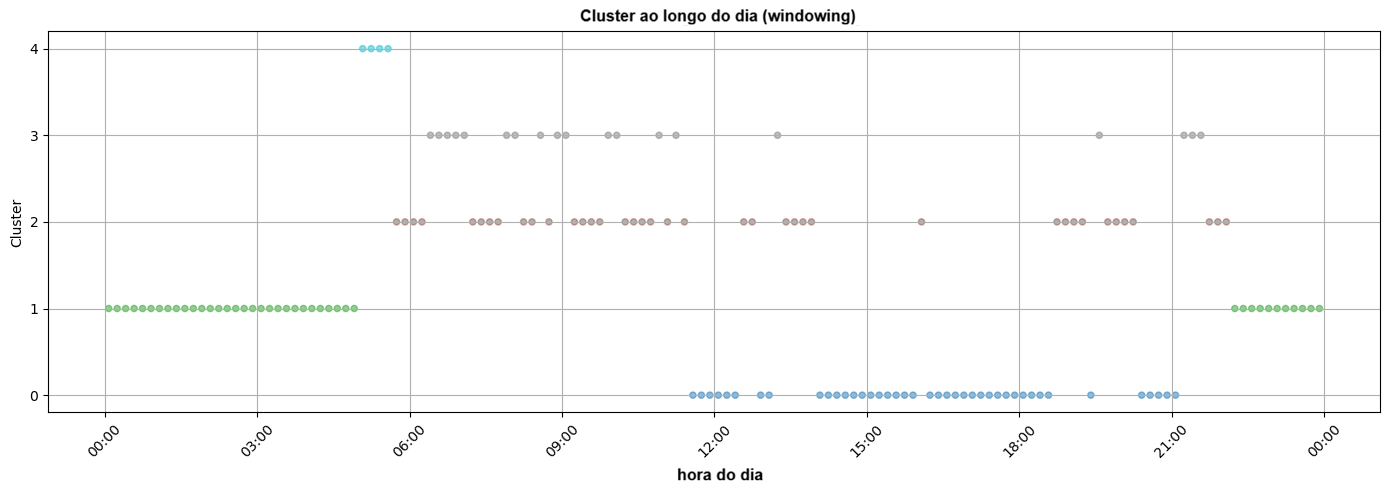
\includegraphics[width=1\textwidth]{ch4/assets/temporalherarquicojanela.png}
\caption{Distribuição temporal diária dos clusters do Clustering Hierárquico ($k=5$, janelas de 10 min) ao longo de uma jornada.}
\label{fig:temporal_hier_janela}
\end{figure}

O Clustering Hierárquico treinado com os dados agregados em janelas de 10 minutos identificou cinco estados fisiológicos coerentes, cuja interpretação resultou da análise conjunta da assinatura das variáveis e da respetiva distribuição temporal. O cluster \textit{Repouso Total} concentra-se durante o período noturno, apresentando baixos níveis de atividade física e frequência cardíaca e elevados valores de \textit{Sleep Stage}. Após o despertar surge o cluster \textit{Despertar e Rotinas Matinais}, caracterizado por maior movimento, mas ainda com reduzida ativação fisiológica. Durante grande parte da jornada laboral predomina o cluster \textit{Concentração e Trabalho}, distinguido pelo EDA elevado e níveis moderados de atividade, enquanto o cluster \textit{Movimento Ativo} corresponde a deslocações e caminhadas distribuídas ao longo do dia. Por fim, o cluster \textit{Picos de Esforço Físico} ocorre apenas de forma pontual, representando os momentos de maior intensidade física.

Tal como observado no GMM com janelas temporais, a agregação em intervalos de 10 minutos produziu uma evolução temporal dos clusters mais estável e organizada. Os diferentes estados distribuem-se em blocos relativamente bem definidos, reduzindo a alternância constante observada nos modelos treinados com dados ao minuto. Verifica-se ainda uma sequência coerente entre repouso, despertar, atividade moderada, período de trabalho e episódios ocasionais de maior esforço físico, sendo estes últimos os menos frequentes ao longo da jornada. Este comportamento sugere que a agregação temporal atenuou as flutuações instantâneas dos sinais fisiológicos, permitindo ao modelo identificar estados mais consistentes e facilmente interpretáveis.
\end{enumerate}

\subsubsection*{Validação Externa com Dados Experimentais do Empatica}
\label{sec:validacao_externa}

Para complementar a avaliação dos modelos de agrupamento, foi realizado um ensaio de validação externa com dados fisiológicos recolhidos diretamente através de um relógio Empatica EmbracePlus. O objetivo foi verificar se os estados fisiológicos identificados no conjunto de treino também eram reconhecidos em dados independentes, recolhidos de um participante diferente daquele cujos dados foram utilizados no treino. Esta abordagem permite avaliar a capacidade de generalização dos modelos para além da separação matemática observada nos dados originais.

Foram consideradas três situações experimentais distintas: \textbf{atividade física}, incluindo musculação e exercício cardiovascular de elevada intensidade; \textbf{trabalho em computador}, representativo de uma situação de concentração e carga cognitiva; e \textbf{sono}, correspondente a um período prolongado de repouso. Os dados foram recolhidos nos dias 24 e 25 de abril de 2026, abrangendo aproximadamente duas horas de atividade física, duas horas de trabalho em computador e 5~h~46~min de sono.

Os dados experimentais foram submetidos ao mesmo \textit{pipeline} de pré-processamento utilizado na construção dos modelos. Foram, assim, aplicados o tratamento de valores omissos, a deteção e o tratamento de anomalias e \textit{outliers}, a normalização e o \textit{scaling}, bem como a codificação das variáveis categóricas. Nos modelos GMM foi ainda aplicada a transformação PCA correspondente. Após este processamento, os dados foram introduzidos nas cinco configurações de inferência previamente preparadas: GMM com dados originais ($k=9$), GMM Restrito com dados originais ($k=4$), GMM com janelas de 10 minutos ($k=5$), Árvore de Decisão treinada para reproduzir o Clustering Hierárquico com dados originais ($k=5$) e Árvore de Decisão treinada para reproduzir o Clustering Hierárquico com janelas de 10 minutos ($k=5$). Como o Clustering Hierárquico não permite atribuir diretamente novos dados a um cluster sem recalcular a estrutura de agrupamento, foram utilizadas as respetivas Árvores de Decisão para realizar a inferência nos dados experimentais. Os modelos não foram reajustados aos dados experimentais, permitindo avaliar diretamente a sua capacidade de generalização.

A avaliação foi baseada na interpretação fisiológica atribuída anteriormente a cada \textit{cluster}. Para cada modelo e situação experimental foram definidos os \textit{clusters} esperados. Por exemplo, no GMM com dados originais ($k=9$), os \textit{clusters} 0 e 5 foram associados ao sono profundo, os \textit{clusters} 3, 4 e 8 à atividade física e os \textit{clusters} 2, 6 e 7 ao trabalho ou à concentração. Uma previsão foi considerada correta quando pertencia ao conjunto de \textit{clusters} compatível com a atividade experimental; caso contrário, foi considerada incorreta. Deste modo, a atribuição não supervisionada de \textit{clusters} foi convertida numa medida de concordância entre o estado fisiológico esperado e o estado identificado pelo modelo.

Nos dados originais, o GMM obteve uma \textit{accuracy} de 75,17\% para a atividade física, 82,64\% para o trabalho em computador e 46,09\% para o sono. O GMM Restrito ($k=4$) alcançou 60,40\% na atividade física, 81,82\% no trabalho em computador e 59,71\% no sono. A Árvore de Decisão treinada para reproduzir o Clustering Hierárquico alcançou 59,73\% na atividade física, 81,82\% no trabalho em computador e 93,04\% no sono. Assim, embora o GMM original tenha apresentado o desempenho mais elevado na identificação da atividade física e o GMM original e o GMM Restrito tenham obtido resultados semelhantes no trabalho em computador, a árvore associada ao modelo hierárquico revelou uma capacidade claramente superior para reconhecer o período de sono.

As Figuras \ref{fig:external_gmm_pc}, \ref{fig:external_gmm_exercise} e \ref{fig:external_gmm_sleep} apresentam a distribuição temporal das previsões do GMM com dados originais ($k=9$) durante o trabalho em computador, a atividade física e o sono, respetivamente. Os pontos verdes representam previsões pertencentes aos \textit{clusters} esperados para cada atividade, enquanto os pontos vermelhos correspondem a previsões fora desse conjunto. Durante o trabalho em computador, predominam as previsões associadas ao estado de trabalho ou concentração, em concordância com a \textit{accuracy} de 82,64\%. Na atividade física, a maioria das previsões concentra-se nos \textit{clusters} associados à atividade física, embora ocorram intervalos classificados como trabalho ou concentração. Durante o sono, observa-se uma presença prolongada de previsões no \textit{cluster} 0, mas também um número considerável de classificações em estados não associados ao sono profundo, o que explica a menor \textit{accuracy} nesta situação.

\begin{figure}[H]
\centering
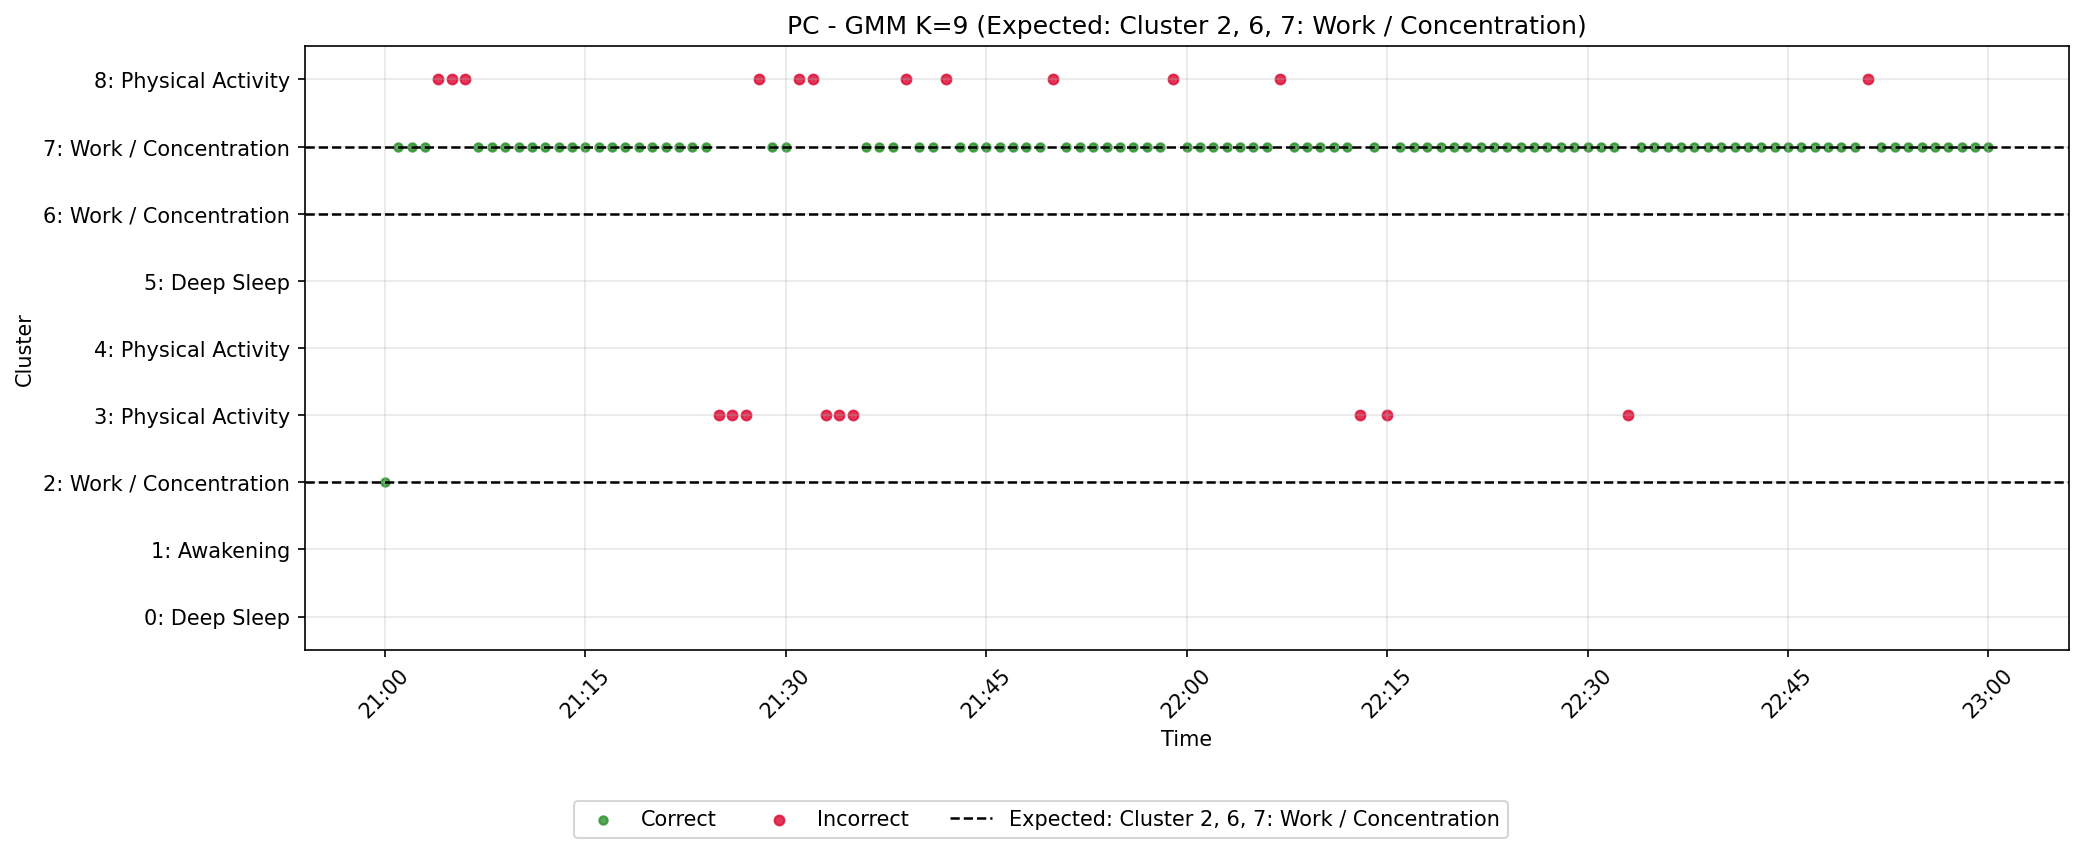
\includegraphics[width=1\textwidth]{ch4/assets/validacao_gmm_trabalho.png}
\caption{Distribuição temporal das previsões do GMM ($k=9$) durante o trabalho em computador.}
\label{fig:external_gmm_pc}
\end{figure}

\begin{figure}[H]
\centering
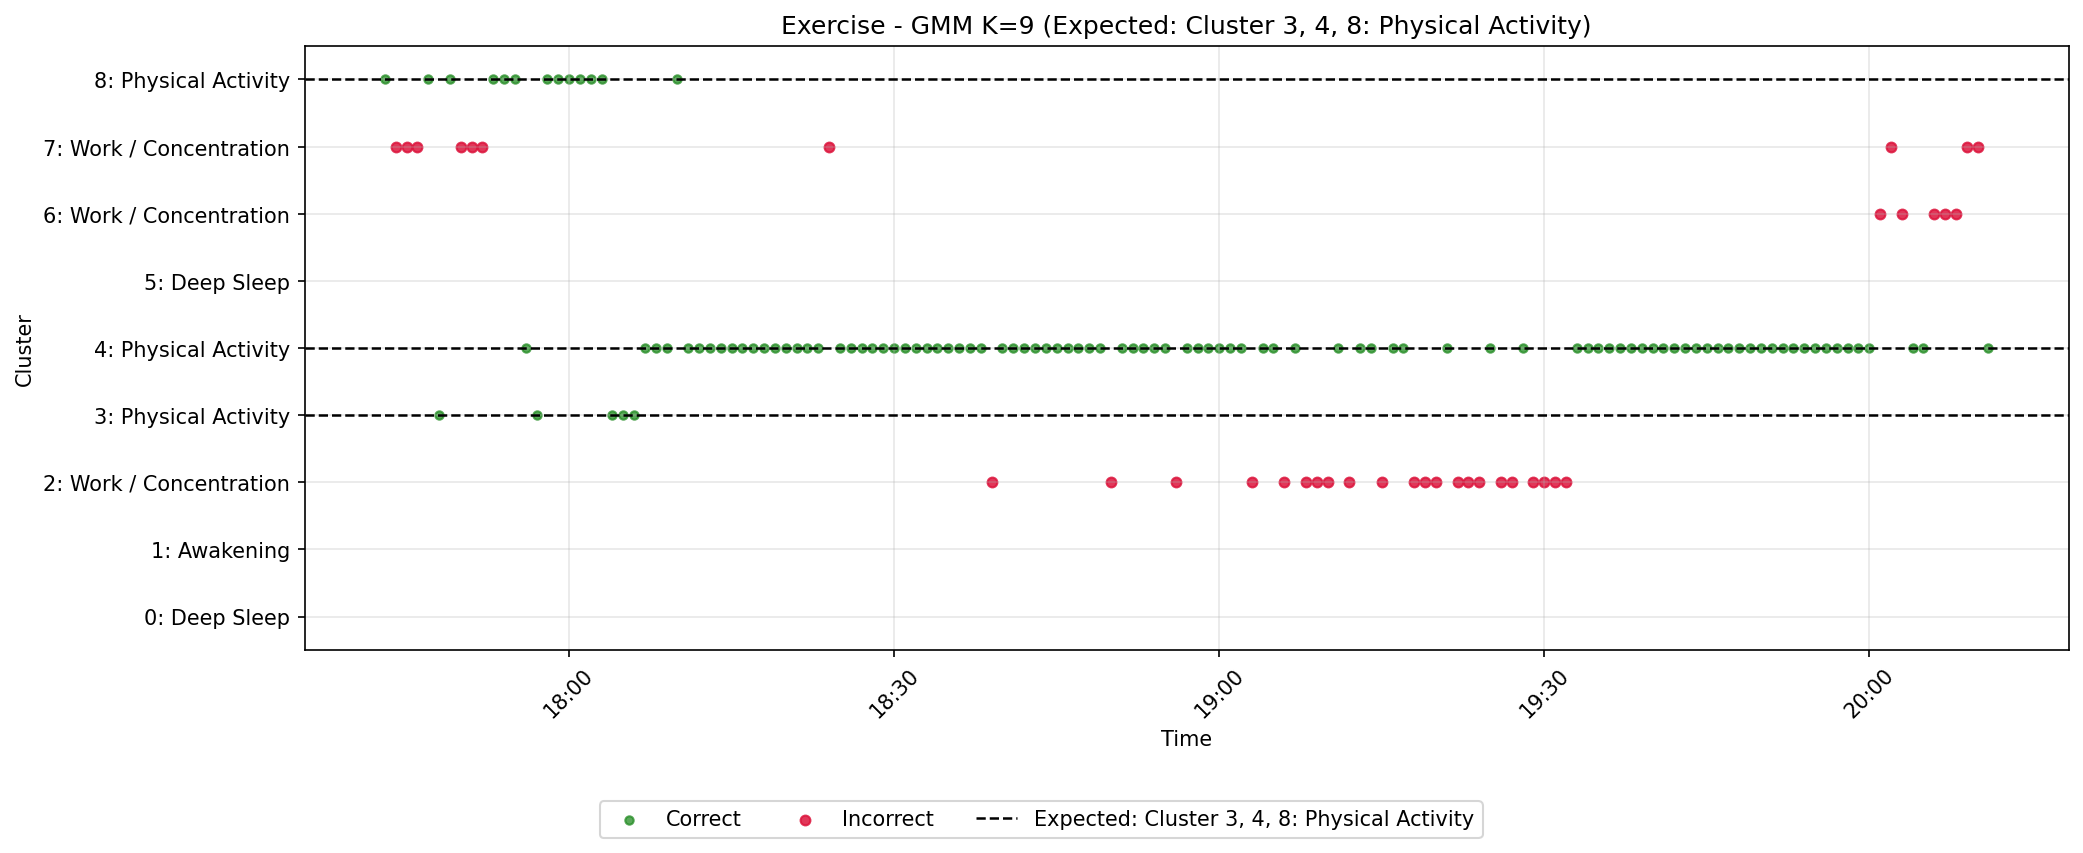
\includegraphics[width=1\textwidth]{ch4/assets/validacao_gmm_atividade_fisica.png}
\caption{Distribuição temporal das previsões do GMM ($k=9$) durante a atividade física.}
\label{fig:external_gmm_exercise}
\end{figure}

\begin{figure}[H]
\centering
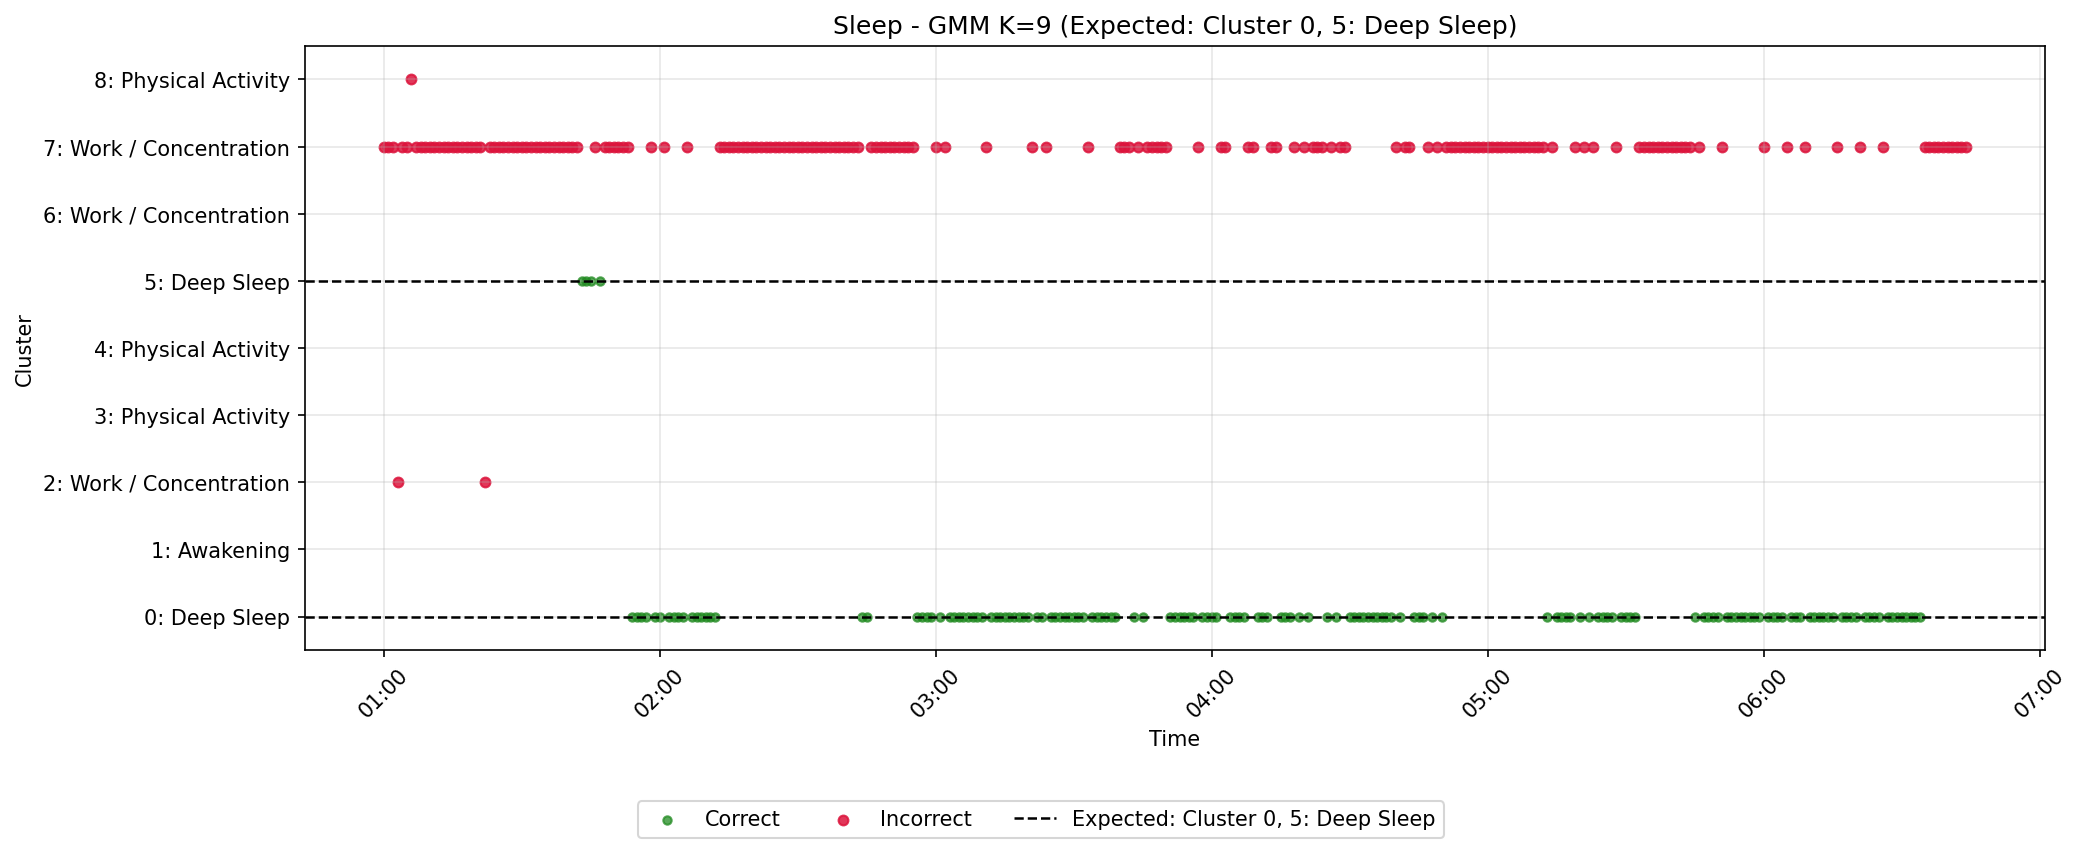
\includegraphics[width=1\textwidth]{ch4/assets/validacao_gmm_sono.png}
\caption{Distribuição temporal das previsões do GMM ($k=9$) durante o período de sono.}
\label{fig:external_gmm_sleep}
\end{figure}

As distribuições temporais das previsões relativas às restantes configurações dos modelos encontram-se disponíveis no \hyperref[AppendixB]{\textbf{Apêndice B}}.

Para os modelos baseados em janelas temporais de 10 minutos, o GMM obteve uma \textit{accuracy} de 26,67\% na atividade física, 76,92\% no trabalho em computador e 51,43\% no sono. A Árvore de Decisão treinada para reproduzir o Clustering Hierárquico com janelas apresentou 0,00\% na atividade física, 23,08\% no trabalho em computador e 100,00\% no sono. A agregação temporal não produziu, portanto, uma melhoria uniforme no reconhecimento das atividades. Embora tenha favorecido claramente a identificação do sono através da árvore associada ao modelo hierárquico, que classificou corretamente as janelas avaliadas, a mesma representação dificultou a identificação da atividade física e do trabalho em computador. A tabela com todos os resultados da validação externa pode ser consultada na Tabela \ref{tab:validacao_externa}.

\begin{table}[H]
\centering
\caption{Accuracy da validação externa para as diferentes configurações dos modelos.}
\label{tab:validacao_externa}
\small
\begin{tabular*}{.95\textwidth}{@{} p{.38\linewidth} p{.17\linewidth} p{.17\linewidth} p{.14\linewidth} @{}}
\toprule
\textbf{\footnotesize Modelo} & \textbf{Atividade física} & \textbf{Trabalho/PC} & \textbf{Sono} \\
\midrule
{\footnotesize GMM ($k=9$)} & 75,17\% & 82,64\% & 46,09\% \\
{\footnotesize GMM Restrito ($k=4$)} & 60,40\% & 81,82\% & 59,71\% \\
{\footnotesize Árvore de Decisão (Hierárquico, $k=5$)} & 59,73\% & 81,82\% & 93,04\% \\
{\footnotesize GMM, janelas ($k=5$)} & 26,67\% & 76,92\% & 51,43\% \\
{\footnotesize Árvore de Decisão (Hierárquico, janelas, $k=5$)} & 0,00\% & 23,08\% & 100,00\% \\
\bottomrule
\end{tabular*}
\end{table}

Em conjunto, os resultados da validação externa mostram que nenhuma configuração apresentou o melhor desempenho em todas as situações fisiológicas. O GMM com dados originais revelou o comportamento mais equilibrado na identificação da atividade física e do trabalho em computador, enquanto o Clustering Hierárquico com dados originais se destacou no reconhecimento do sono. O GMM Restrito ($k=4$) apresentou um desempenho intermédio, melhorando a identificação do sono face ao GMM original, mas ficando abaixo do Clustering Hierárquico nessa atividade. A utilização de janelas de 10 minutos reforçou a identificação de estados prolongados de repouso no modelo hierárquico, mas prejudicou a discriminação de atividades de curta duração ou mais variáveis, como o exercício físico e determinadas situações de trabalho. Estes resultados confirmam que a qualidade dos modelos de agrupamento não deve ser avaliada exclusivamente através de métricas internas, como o \textit{Silhouette Score} ou o WCSS, devendo incluir também a aplicação a dados independentes e experimentalmente controlados.

\clearpage
\section{Análise e Conclusões de Resultados}
\label{sec:analise_conclusoes}

Esta secção analisa e interpreta os principais resultados experimentais apresentados neste capítulo. Primeiro, são discutidos os modelos supervisionados de regressão e classificação desenvolvidos com os dados da banda peitoral Polar H10. De seguida, são analisados os modelos não supervisionados de agrupamento (\textit{clustering}) aplicados aos dados multimodais e de atividade do relógio inteligente Empatica EmbracePlus.

\subsection*{Conclusões do Polar H10 (Modelos Supervisionados):}

\subsection*{1. Interpretação do FatigueIndex}

O desempenho excecional dos modelos de regressão, particularmente da Regressão Linear ($R^{2} = 1.0$), explica-se pelo facto de o \textit{FatigueIndex} ter sido construído através de uma \textbf{fórmula heurística} baseada nos próprios atributos do \textit{dataset}. Uma vez que a variável alvo é uma combinação linear ponderada de métricas como \texttt{HR\_mean}, \texttt{RMSSD} e \texttt{ECG\_energy}, é expectável que os modelos consigam identificar e reconstruir esta relação matemática com facilidade.

Por isso, a questão principal não é apenas saber qual é o melhor algoritmo. Os resultados mostram que os modelos conseguem reproduzir com eficácia tanto o \textbf{valor contínuo} do \textit{FatigueIndex} como as \textbf{categorias} definidas a partir desse índice. A capacidade de identificar corretamente diferentes níveis de ativação ou de fadiga depende sobretudo de quão bem o próprio índice representa esses estados na vida real do trabalhador. Ainda assim, os resultados do estudo com dados externos sugerem que as previsões e a representação do índice foram coerentes com diferenças entre períodos de menor ativação, atividade moderada e maior esforço físico.

O \textit{FatigueIndex} deve, portanto, ser compreendido como uma tentativa heurística de representar diferentes níveis de fadiga e ativação, estando mais próximo de um identificador de níveis relativos de atividade física e estado fisiológico. As categorias LOW, MED e HIGH constituem uma referência que permite organizar os sinais numa escala comum, comparar participantes e modelos, bem como acompanhar alterações do estado fisiológico no Gémeo Digital.

\subsection*{2. Importância das Características \textmd{\textit{(estudo de Ablação)}}}

O estudo de ablação mostrou que a \textbf{combinação das características de ECG, HR/R-R e temporais} é a mais robusta para a generalização entre trabalhadores. No XGBoost, o cenário completo alcançou uma Accuracy média de 0,8817, uma Balanced Accuracy de 0,8547 e um Macro-F1 de 0,8310. Quando foram removidas as características de ECG, estes valores diminuíram para 0,6566, 0,6413 e 0,5991, respetivamente. Quando foram removidas as características de HR/R-R e temporais, mantendo apenas as características derivadas do ECG, a Accuracy foi de 0,6783, mas a Balanced Accuracy e o Macro-F1 diminuíram para 0,6136 e 0,5892.

Assim, as características derivadas do ECG podem manter alguma capacidade discriminativa quando utilizadas isoladamente, mas não substituem a combinação multimodal na avaliação LOSO. Por este motivo, no âmbito do projeto, não seria recomendável prescindir de nenhuma das principais medições fisiológicas (ECG, HR ou RR). Por sua vez, o resultado intra-individual anterior, no qual o XGBoost atingiu 97,65\% sem HR/R-R, deve ser interpretado como evidência de reprodução das categorias do \textit{FatigueIndex} num único trabalhador, e não como prova de reconhecimento independente da fadiga ou de um alerta de segurança clinicamente fiável. A utilidade de características como \texttt{ECG\_missing\_peaks} e \texttt{ECG\_samp\_ent} deverá ser confirmada em avaliações com mais participantes e com referências fisiológicas independentes.

\subsection*{3. Generalização e Validação Externa}

Na avaliação LOSO, o \textbf{XGBoost apresentou o melhor desempenho médio} entre os modelos testados, com Accuracy de 0,88, Balanced Accuracy de 0,85 e Macro-F1 de 0,83. A classe MED foi a mais difícil de identificar, com recall médio de 0,74, enquanto LOW e HIGH alcançaram recalls de 0,91 e 0,92. Esta diferença indica que os estados intermédios são mais difíceis de separar dos estados adjacentes, constituindo uma limitação importante para a interpretação das categorias derivadas do \textit{FatigueIndex}.

A dificuldade na identificação da classe MED poderá estar parcialmente relacionada com a definição dos limiares P33 e P66. Como trabalho futuro, deverão ser avaliadas diferentes divisões percentílicas, verificando se a alteração dos limites permite melhorar a separação entre categorias sem introduzir desequilíbrio entre classes ou sobreajuste.

A validação externa com o Polar H10 permitiu observar o comportamento temporal dos modelos num novo participante, embora sem etiquetas independentes do nível real de fadiga. No registo completo \texttt{PC}, a Regressão Logística apresentou a maior concordância contextual (90,85\%), enquanto no registo completo \texttt{EXERCISE} o melhor resultado foi obtido pelo SVM (78,15\%). Na análise dos intervalos específicos, os quatro modelos foram compatíveis com o contexto em todas as janelas da caminhada na passadeira, enquanto no trote o Random Forest apresentou a maior concordância (90\%), com apenas dez janelas avaliadas. Estes resultados reforçam a interpretação das categorias LOW, MED e HIGH como uma representação aproximada de diferentes estados físicos e níveis de atividade, mas devem ser entendidos como evidência de coerência contextual, e não como métricas de exatidão clínica ou validação independente da fadiga.

Em síntese, os modelos demonstraram capacidade para reconhecer padrões fisiológicos em trabalhadores diferentes, sobretudo quando combinam várias características, embora o desempenho varie entre pessoas e seja inferior na categoria intermédia MED. A utilidade destes modelos deverá ser confirmada em estudos com mais participantes e com medidas de referência independentes, capazes de avaliar de forma mais direta os diferentes níveis de fadiga.

\subsection*{4. Limitações dos Modelos e dos Dados}

Apesar da capacidade de generalização observada na avaliação LOSO, a variabilidade entre trabalhadores continua a ser relevante: o desempenho do XGBoost foi elevado em vários participantes, mas diminuiu consideravelmente nos trabalhadores W07 e W08, enquanto o resultado perfeito de W09 deve ser interpretado com cautela devido às suas apenas 16 janelas. Esta heterogeneidade não invalida os resultados obtidos, mas mostra que o desempenho não é uniforme entre trabalhadores e que a aplicação a novos utilizadores poderá beneficiar de calibração ou validação adicional, reforçando a necessidade de personalizar os modelos de IA dentro do ecossistema do Gémeo Digital.

A qualidade dos dados constitui igualmente uma limitação importante. A presença de \textbf{valores omissos} pode reduzir o número de janelas disponíveis para análise e comprometer a estabilidade das características extraídas. Do mesmo modo, falhas na colocação do dispositivo, na transmissão dos dados ou na deteção dos sinais podem introduzir artefactos ou eliminar informação relevante dos sinais de ECG, HR e R-R. Como consequência, parte das diferenças observadas entre trabalhadores e entre modelos poderá estar relacionada com a qualidade da aquisição, e não apenas com os estados fisiológicos representados pelo \textit{FatigueIndex}. Esta limitação é particularmente relevante porque o índice é calculado a partir das próprias características fisiológicas utilizadas pelos modelos.

Por isso, as próximas experiências deverão acompanhar de forma sistemática a quantidade e a origem dos valores omissos, bem como as falhas ocorridas durante a recolha. Será também necessário verificar se os modelos mantêm um desempenho estável quando os dados são obtidos em condições de aquisição mais controladas e com diferentes participantes. Esta análise permitirá distinguir melhor as limitações do modelo das limitações introduzidas pelo processo de recolha dos sinais.

\subsection*{5. Estratégia de Desenvolvimento dos Modelos}

Os resultados mostram uma diferença importante entre os cenários intra-individual e inter-individual. Quando o modelo é treinado e testado com dados do mesmo trabalhador, o desempenho é elevado, mas isso não garante que o modelo reconheça corretamente os estados de outros trabalhadores. Na avaliação LOSO, os modelos demonstraram uma capacidade de generalização mais realista, embora o desempenho não tenha sido perfeito e tenha variado entre indivíduos.

Esta diferença deixa em aberto duas estratégias para o desenvolvimento do Gémeo Digital. Uma possibilidade consiste em treinar \textbf{modelos personalizados} para cada trabalhador, utilizando uma fase inicial de calibração. Outra consiste em continuar a recolher dados de mais participantes e a avaliar modelos com maior \textbf{capacidade de generalização}. A primeira estratégia poderá oferecer um desempenho mais elevado para cada utilizador, enquanto a segunda poderá facilitar a aplicação do sistema a novos trabalhadores sem depender de uma calibração extensa.

\subsection*{6. Outras Abordagens de Modelação e Trabalho Futuro}

Até ao momento, esta investigação focou-se em métodos de aprendizagem supervisionada, que demonstraram resultados sólidos. Como trabalho futuro, poderão ser avaliados modelos de \textbf{Deep Learning}, como LSTM, Bi-LSTM e 1D-CNN, para extrair padrões temporais e morfológicos mais complexos das séries temporais do Polar H10. Estas arquiteturas são compatíveis com os dados de ECG, HR e RR, mas não foram implementadas nesta investigação e exigiriam uma amostra maior para avaliar o risco de sobreajuste e a capacidade de generalização para novos trabalhadores.

Em paralelo, a implementação de métodos de aprendizagem não supervisionada, como o \textbf{Clustering}, constituiria uma abordagem exploratória para organizar os dados sem depender diretamente de uma fórmula pré-definida. Ao agrupar os sinais por semelhança estatística, seria possível avaliar em que medida os grupos gerados pela máquina se correspondem com as categorias do \textit{FatigueIndex} heurístico. Esta comparação entre métodos supervisionados e não supervisionados poderia complementar a análise atual, permitindo identificar padrões alternativos de categorização do estado do trabalhador.

\subsection*{Conclusões do Relógio EmbracePlus (Modelos Não Supervisionados):}

\subsection*{1. Efeito da Agregação Temporal}

A comparação entre os dados ao nível do minuto e os dados agregados em janelas temporais de 10 minutos permitiu avaliar o efeito da resolução temporal nos agrupamentos obtidos. Nos dados originais, os algoritmos de clustering foram expostos a maior variabilidade instantânea dos sinais. No GMM, a agregação temporal reduziu o número de agrupamentos de $k=9$ para $k=5$ e aumentou o Silhouette Score de 0.3475 para 0.3742. No Clustering Hierárquico, o Silhouette Score também aumentou de 0.3959 para 0.4132. Contudo, nos dados externos, a agregação não produziu ganhos uniformes: melhorou o reconhecimento do sono no Clustering Hierárquico, mas reduziu o desempenho na atividade física e no trabalho em computador. Assim, a \textbf{agregação temporal} pode tornar os agrupamentos mais compactos, mas o seu efeito na capacidade de distinguir diferentes atividades depende do modelo e da situação analisada.

\subsection*{2. Efeito da Redução de Dimensionalidade}

A metodologia aplicada revelou um compromisso importante na fase de engenharia de características. Para o GMM, foi utilizado o \textit{Principal Component Analysis} (PCA), uma técnica que reduz o número de variáveis sem eliminar a maior parte da informação presente nos dados. Nos dados ao minuto, foram suficientes 6 componentes principais, enquanto nas janelas temporais foram suficientes 4, mantendo-se em ambos os casos cerca de 90\% da variância original. Esta redução tornou o conjunto de dados mais simples e facilitou o cálculo da distribuição probabilística utilizada pelo GMM, bem como a aplicação do critério BIC para comparar diferentes números de agrupamentos.

No caso do Clustering Hierárquico, não foi aplicada esta redução. O modelo foi treinado diretamente com as 12 características originais normalizadas, tanto nos dados ao minuto como nas janelas temporais. Neste caso, o valor mais elevado de Silhouette Score foi 0.4132, indicando uma melhor coesão interna dos agrupamentos quando o conjunto completo de características foi mantido. Assim, os resultados sugerem que o PCA foi útil para simplificar a modelação do GMM, enquanto o Clustering Hierárquico beneficiou da utilização das características originais.

\subsection*{3. Escolha do Número de Agrupamentos}

Por fim, os resultados permitiram discutir a diferença entre a seleção do número de clusters com base em critérios matemáticos e a necessidade de obter agrupamentos fáceis de interpretar no contexto do Gémeo Digital Humano. Para os dados ao minuto, o critério BIC selecionou teoricamente $k=9$ clusters para o GMM. Contudo, a análise das assinaturas sugeriu que esta configuração poderia fragmentar excessivamente os dados, criando grupos associados a pequenas variações entre estados semelhantes. A utilização de um número mais reduzido de clusters, como no GMM Restrito ($k=4$) ou no Clustering Hierárquico ($k=5$), facilitou a interpretação dos agrupamentos, embora com alguma redução do Silhouette Score. Estes resultados sugerem que, em aplicações de monitorização do estado fisiológico, a escolha do número de clusters deve considerar não apenas a qualidade matemática do agrupamento, mas também a \textbf{interpretabilidade e estabilidade em dados externos}.

\subsection*{4. \textit{Árvores de Decisão}: Interpretação e Inferência dos Agrupamentos}

Um dos desafios fulcrais na modelação não supervisionada consiste em traduzir limites multidimensionais em regras compreensíveis e utilizáveis. A validação paralela com \textbf{Árvores de Decisão} mostrou que é possível reproduzir com elevada concordância as decisões do Clustering Hierárquico. No cenário ao nível do minuto, a árvore de decisão necessitou de uma profundidade máxima de 8 níveis, atingindo 98.61\% de precisão no treino e 92.01\% em validação cruzada (5-Fold CV). Com janelas de 10 minutos, foi suficiente uma profundidade máxima de 5 níveis, com 93.06\% de precisão no treino e 83.92\% em validação. Estes resultados indicam que as árvores conseguem aproximar as fronteiras definidas pelo modelo hierárquico através de um conjunto reduzido de regras, mantendo uma elevada concordância com os agrupamentos de referência.

Esta propriedade é particularmente relevante para o projeto CRIARTE. Pela sua natureza, o Clustering Hierárquico não dispõe de uma operação direta de inferência para uma nova observação: para incorporar novos dados, é necessário recalcular ou reestruturar o agrupamento. Uma Árvore de Decisão treinada com as etiquetas produzidas pelo modelo hierárquico pode, por isso, funcionar como uma camada de inferência mais rápida, aplicável em tempo real e com menor custo computacional. As regras extraídas podem ainda servir de base à criação de regras heurísticas mais simples e eficientes para o Gémeo Digital, desde que a sua concordância com o modelo de referência seja monitorizada. Assim, as árvores constituem uma forma rápida e interpretável de reproduzir os agrupamentos identificados e de apoiar inferências operacionais no projeto.

\subsection*{5. Validação Externa}

A validação externa demonstrou que as configurações de inferência conseguiram reconhecer, com diferentes níveis de desempenho, padrões fisiológicos presentes nos dados de um participante que não foi utilizado no treino. Este resultado é relevante, uma vez que as configurações foram aplicadas sem reajuste aos dados experimentais, permitindo avaliar a sua \textbf{capacidade de generalização} para além da estrutura observada no conjunto original. Ao mesmo tempo, nenhuma configuração apresentou o melhor desempenho nas três situações avaliadas. Isto mostra que os resultados variam consoante o participante e a atividade realizada, devido às diferenças fisiológicas e comportamentais entre as pessoas. Assim, a utilização das árvores como camada de inferência rápida é promissora, mas deve continuar a ser estudada e reforçada com dados independentes.

Entre os modelos GMM, a configuração original apresentou o desempenho mais equilibrado nas diferentes atividades, enquanto a versão restrita produziu resultados intermédios. A utilização de janelas de 10 minutos não melhorou de forma consistente o reconhecimento das atividades, embora o GMM possa realizar diretamente inferências sobre novos dados. Assim, o desempenho deste modelo dependeu tanto da atividade analisada como da representação temporal utilizada.

Nas configurações baseadas no Clustering Hierárquico, a inferência externa foi realizada pelas respetivas Árvores de Decisão. Estas apresentaram um comportamento particularmente favorável no reconhecimento do sono, sobretudo com janelas temporais, mas tiveram mais dificuldades na identificação da atividade física e do trabalho em computador. Apesar disso, mantêm interesse como uma forma rápida de reproduzir as decisões do clustering. Será necessário testar tanto as árvores como os modelos GMM com mais participantes e em diferentes situações, para confirmar se conseguem manter um funcionamento consistente em tempo real.

Em conjunto, estes resultados sugerem que, no âmbito do projeto CRIARTE, poderá ser vantajoso adotar uma \textbf{abordagem híbrida de inferência}, combinando diferentes modelos em vez de utilizar uma única solução para todas as atividades. Por exemplo, o sistema poderia recorrer ao modelo que apresenta melhor comportamento em cada situação, utilizando o GMM quando este distinguir melhor uma determinada atividade e as Árvores de Decisão quando for necessária uma inferência rápida baseada nos agrupamentos hierárquicos. Esta estratégia poderá aumentar a flexibilidade do Gémeo Digital, mas deverá ser estudada com mais participantes e atividades antes de ser implementada como regra geral.

\subsection*{6. Limitações dos Dados e Trabalho Futuro}

Apesar dos resultados promissores obtidos com os dados externos, a validação do Empatica EmbracePlus foi realizada com dados de um \textbf{único participante}. Isto aconteceu porque o projeto dispunha de apenas um relógio Empatica EmbracePlus e porque cada recolha exigia uma simulação experimental financiada pelo próprio projeto. Como o dispositivo tem um custo elevado e as simulações exigem recursos, não foi possível recolher dados de mais participantes nem repetir as experiências em muitas condições diferentes. Os resultados devem, por isso, ser interpretados como uma avaliação inicial, não sendo possível garantir que os agrupamentos e as regras das árvores apresentem o mesmo comportamento noutras pessoas.

Como trabalho futuro, será necessário aumentar gradualmente o número de participantes e repetir as recolhas em diferentes atividades e condições experimentais. Será também importante verificar se os agrupamentos identificados pelos modelos correspondem às atividades realmente realizadas durante as experiências, como períodos de repouso, trabalho, exercício físico e sono. Para isso, será necessário utilizar registos das atividades ou avaliações obtidas por outro procedimento, em vez de analisar apenas os sinais utilizados pelos próprios modelos. Esta comparação permitirá perceber se os modelos identificam padrões associados a diferentes atividades ou se estão apenas a organizar matematicamente os dados do participante analisado.

Outra possibilidade consiste em substituir ou complementar o \textit{clustering} por modelos supervisionados de \textit{Machine Learning} e \textit{Deep Learning}, aproveitando a diversidade de variáveis recolhidas pelo relógio. Para isso, seria necessário recolher, durante a experiência, avaliações periódicas da fadiga, do stress ou de outro estado relevante, através de perguntas ou escalas respondidas pelo próprio participante. Essas respostas poderiam fornecer as etiquetas dos dados e permitir treinar modelos capazes de estimar diretamente os níveis de fadiga, stress ou outros estados definidos pelo projeto em tempo real.


